\documentclass[11pt]{article}

% ===========================================================================
%  Paper 1
%  From Microprice to Microdiffusion
%  in Limit Order Books
% ===========================================================================

\usepackage[utf8]{inputenc}
\usepackage[T1]{fontenc}
\usepackage{lmodern}
\usepackage{amsmath,amssymb,amsthm,mathtools}
\usepackage{bm}
\usepackage[margin=1in]{geometry}
\usepackage{graphicx}
\usepackage{booktabs}
\usepackage{array}
\usepackage{multirow}
\usepackage{siunitx}
\usepackage{placeins}
\usepackage{tikz}
\usetikzlibrary{arrows.meta, positioning, fit, backgrounds}
\usepackage{hyperref}
\usepackage[round]{natbib}
\hypersetup{colorlinks=true, linkcolor=black, citecolor=black, urlcolor=blue}

% existing figures live in the empirical output tree; new/gap figures in ./figures
\graphicspath{{figures/}{../fluid-mechanics/empirical/output/figures/}}

% compiling placeholder for figures not yet produced (clearly marked)
\newcommand{\figplaceholder}[1]{%
  \fbox{\parbox[c][4.2cm][c]{0.82\linewidth}{\centering\itshape
  [Figure to be produced]\\[2pt]\normalfont\small #1}}}

% theorem-like environments
\theoremstyle{plain}
\newtheorem{assumption}{Assumption}
\newtheorem{proposition}{Proposition}
\theoremstyle{definition}
\newtheorem{definition}{Definition}

% notation shortcuts (semantic, not abbreviations of prose)
\newcommand{\E}{\mathbb{E}}
\newcommand{\Var}{\operatorname{Var}}
\newcommand{\Cov}{\operatorname{Cov}}
\newcommand{\given}{\,\vert\,}
\newcommand{\dd}{\mathrm{d}}
\newcommand{\Real}{\mathbb{R}}
\newcommand{\Norm}{\mathcal{N}}
\newcommand{\GIG}{\mathrm{GIG}}
\newcommand{\GH}{\mathrm{GH}}
\newcommand{\axx}{a_{xx}}

\title{\bfseries From Microprice to Microdiffusion\\[0.2em]
Heavy-Tailed Price Diffusion in Limit Order Books\\[0.35em]
{\large A Microstructure-Native Second-Moment Model}}

\author{%
Geoffrey Ducournau$^{\dag}$
\quad Yibo Wang$^{\ddag}$
\quad Jinliang Li$^{\dag}$\thanks{Corresponding author. Email: jll@tsinghua.edu.cn}\\[0.5em]
\small $^\dag$School of Economics and Management, Tsinghua University, Beijing, China\\
\small $^{\ddag}$Sorbonne University, Paris, France
}
\date{\today}

\begin{document}
\maketitle

% ===========================================================================
\begin{abstract}
\noindent
The microprice made the visible limit order book a model of short-horizon price
direction. This paper extends that idea from direction to risk. We introduce the
\emph{microdiffusion}, a state-dependent second-moment surface $\axx(I,S)$ indexed by
best-level imbalance and relative spread, and combine it with the Stoikov microprice
drift in the event-time equation
$\Delta x_n=b_x(I_n,S_n)+\sqrt{\axx(I_n,S_n)}\,\eta_n$. Unlike GARCH, realized-volatility,
or latent stochastic-volatility models, the conditional scale in this equation is not
inferred from the history of returns. It is read directly from the contemporaneous
limit order book. The result is an observable, interpretable, and transferable
microstructure-native model of the full next-move distribution.

Using tick-by-tick data from the Qatar Stock Exchange, a thin frontier-market venue
where short-horizon tail risk is economically important, we show that the diffusion
surface is a stable structural object. Its spread-driven level transfers across
disjoint trading days, across instruments, and across calm and stressed volatility
regimes. Holding spread-in-ticks fixed, imbalance magnitude symmetrically raises
conditional variance, revealing a second-moment role for order-book imbalance that is
distinct from its signed first-moment role in the microprice. The Gaussian version of
the model captures local scale but misses abrupt moves. Replacing the innovation with
a symmetric Generalized Hyperbolic law delivers a tail-calibrated predictive
distribution, materially reduces Gaussian far-tail under-coverage in intraday VaR
backtests, and preserves the economic interpretability of $\axx(I,S)$ as the book-state
scale. Against return-history
benchmarks, the model matches jointly estimated GARCH-$t$ while providing something
return-history models do not: an ex-ante decomposition of short-horizon price risk
directly from the current limit order book. The paper therefore extends the microprice
program from conditional drift to conditional diffusion and provides a practical
state-indexed model for heavy-tailed price risk in thin electronic markets.
\end{abstract}

% ===========================================================================
\clearpage
\section{Introduction}
\label{sec:intro}

Order-book imbalance, the normalised difference between the volume resting at the
best bid and the volume resting at the best offer, is among the most widely used
short-horizon predictors in market microstructure. Its modern formalisation is the
\emph{microprice} of \citet{stoikov2018}. The microprice adjusts the mid-price by a
quantity learned from the imbalance and the spread. Conceptually, it is a
state-dependent answer to a simple question: given the current book, where is the
next mid-price expected to be? In moment language, it is a model of the
\emph{conditional first moment} of the next price increment.

That first moment is important, but it is not the whole distribution. Two book
states can have the same expected next move and very different uncertainty around
that move: one state may produce a tight cluster of small price changes, while
another may produce occasional large jumps. A usable stochastic model therefore
needs the conditional \emph{second} moment as well as the conditional mean. In
continuous-time language, drift must be accompanied by diffusion. The microprice
literature has developed the drift side in considerable depth; the conditional
diffusion of the price, \emph{as a function of the same book state}, has received
far less attention. This paper is about that object. We define it, estimate it,
show that it is structurally real rather than an artifact of sampling, assemble it
with the Stoikov drift into a single state-dependent price equation, and determine
the distribution that the equation's random innovation must have. In one sentence:
we introduce the \emph{microdiffusion}: a microstructure-native diffusion surface,
estimated directly from the visible limit order book rather than from the history of
returns, that turns the microprice framework from a conditional-drift model into a
full conditional-distribution model for short-horizon price risk.
This distinction is central. The scale in our equation is not a latent volatility
state inferred from option prices, a realized-volatility summary, or a GARCH-type
filter of past returns. It is an observable function of the current market
microstructure, read from the book before the next move occurs.

The QSE setting is not only a limitation on external scope; it is also the environment in
which the risk problem is sharpest. In a thin, coarse-tick frontier market, exits are costly,
the book can become one-sided, and a short-horizon Gaussian band can be most misleading
exactly when liquidity is hardest to replace. A state-conditional tail model is therefore not
just a statistical refinement. It is a way to measure the next-move risk faced by a trader or
risk manager before the move occurs, using the same visible book state that determines whether
that risk can be exited cheaply.

Three features distinguish the conditional diffusion we study from the large
existing literature on time-varying volatility, and they are worth stating at the
outset because they define the contribution. First, our object is
\emph{state-indexed} rather than time-indexed. Autoregressive conditional
heteroskedasticity models \citep{engle1982,bollerslev1986} make the conditional
variance a function of the recent past of the return series itself; realized-volatility
and stochastic-volatility models likewise infer volatility from past variation,
option prices, or latent state dynamics. Here the conditional variance is a function
of the \emph{contemporaneous} state of the order book, $(I,S)$, observed before the
move occurs. It is a surface over book states, not a recursion in time. Second, the transferable component of that surface is explicit:
the spread-driven level reappears across trading days and instruments, while the
tick-controlled imbalance shape is a real contemporaneous second-moment effect whose
day-to-day transfer is weak. Third, the diffusion is presented \emph{coupled
to the drift}: the microprice supplies the conditional mean and our surface
supplies the conditional variance, and the two are assembled into one equation of
motion for the price.

The empirical argument follows the same sequence. (i) Consistent with the microprice construction, the
conditional drift of the price is, to a good approximation, a function of the
imbalance and the spread alone and does not require the price level; the third
state coordinate is the variable that diffuses, not the one that steers. (ii) The
conditional price diffusion $\axx(I,S)$ is a stable function of the book state, but the
stability is not uniform across components: the full surface has high split-half reliability
and positive cross-day transfer, the spread axis carries most of the transferable level, and
the tick-controlled imbalance effect moves conditional variance without reliably transferring
as a day-to-day shape.
(iii) The state-dependent event-time stochastic equation built from the drift
and the diffusion has the \emph{right scale} but, under a Gaussian innovation, the
\emph{wrong tails}: it understates the frequency of large moves by a wide margin.
(iv) Modelling the innovation as a symmetric, unit-variance Generalized Hyperbolic
law substantially improves the tail fit, and the fitted tail law performs well on a
fresh temporal split. (v) The scale
and the shape of the move are separately identified and each is necessary: neither
the diffusion surface alone nor a universal heavy-tailed kick alone explains the
data.

The remainder of the paper is organised as follows.
Section~\ref{sec:related} reviews the relevant literature and states the research
questions. Section~\ref{sec:framework} develops the theoretical framework, building
from the microprice drift to the conditional diffusion, the implied stochastic
differential equation, and the distribution of its innovation; all quantities are
defined and all results derived. Section~\ref{sec:data} describes the QSE data and
the estimation and out-of-sample protocols. Section~\ref{sec:results} presents the
empirical results in the order of the framework. Section~\ref{sec:robustness}
collects robustness checks and limitations, Section~\ref{sec:discussion} discusses
the model's scope and uses, and Section~\ref{sec:conclusion} concludes.
Appendix~\ref{app:external} reports the external-sample checks.

% ===========================================================================
\section{Related Work and Research Questions}
\label{sec:related}

\paragraph{Order-book signals and the microprice.}
The predictive content of order-book imbalance for short-horizon price moves is
well documented \citep{ohara1995,hasbrouck2007,gould2013}. \citet{cont2014} relate
price changes to the net flow of order-book events, and \citet{bouchaud2009} survey
the slow, state-dependent way in which supply and demand are reflected in prices.
\citet{stoikov2018} crystallises the imbalance-and-spread signal into the
microprice, a martingale-consistent estimator of the future mid-price that adjusts
the mid by a function of the imbalance and the spread. All of these treat, in our
language, the conditional \emph{drift} of the price. Our concern is the conditional
\emph{diffusion}: the second moment of the price increment as a function of the same
state.

\paragraph{Conditional variance in time-series models.}
The dominant tradition for time-varying volatility is the family of autoregressive
conditional heteroskedasticity models \citep{engle1982,bollerslev1986} and their
realized-volatility successors \citep{andersen2003}, together with related
return-volatility specifications such as \citet{ma2014model}, in which the conditional
variance of a return is driven by the recent history of squared returns. It is
common in this tradition to combine a conditional-variance recursion with a
heavy-tailed innovation, most classically a Student-$t$ \citep{bollerslev1987}. Our
model shares the multiplicative architecture \emph{conditional scale $\times$
unit-variance innovation} with this literature, and we draw on the comparison in
Section~\ref{sec:framework}. The essential difference is the conditioning set: our
conditional variance is a function of the \emph{contemporaneous order-book state},
not of the past of the return series, and it is therefore a cross-sectional surface
that can be transferred across days and, in robustness checks, across instruments. We
make this comparison concrete in Section~\ref{sub:res-garch}, where we show that the
microdiffusion is not a substitute for a GARCH forecast but a complement to it:
it provides an observable and transferable book-state risk decomposition that matches,
rather than dominates, the strongest return-history benchmark once both sides are allowed
heavy-tailed innovations.

\paragraph{Option-implied volatility and latent stochastic volatility.}
A second, complementary tradition begins from option prices rather than from the
limit order book. In the Black--Scholes model \citep{blackscholes1973}, volatility is
constant; in practice, the model is often used as a transform from option prices into
Black--Scholes implied volatilities. The empirical implied-volatility surface is not
flat: it varies with strike and maturity, producing the familiar smile and skew. This
failure of constant volatility motivated two broad modelling responses. Local-volatility
models make the instantaneous variance a deterministic function of calendar time and
price level, calibrated to the option surface \citep{dupire1994}. Stochastic-volatility
models make volatility a latent factor, as in the bivariate diffusions of
\citet{hullwhite1987}, \citet{heston1993}, and the SABR model of \citet{hagan2002},
or a forward-variance curve driven by hidden volatility shocks, as in Bergomi-type
models \citep{bergomi2016}. Schematically, these models write
\[
  \frac{dS_n}{S_n}=\sqrt{v_t}\,dB_t,
  \qquad
  dv_t=\kappa(\bar v-v_t)\,dt+\eta\sqrt{v_t}\,dW_t
  \quad\text{(Heston)}
\]
or replace the Markovian variance diffusion by a rough forward-variance specification,
for example
\[
  v_t=\xi_0(t)\exp\!\left(\eta W_t^H-\frac12\eta^2 t^{2H}\right)
  \quad\text{(rough Bergomi)}.
\]
In both cases $v_t$ is a volatility state to be inferred or calibrated; it is not a
visible order-book variable. More recently, rough-volatility models argue that the
volatility path is much rougher than a standard diffusion. This matters because
standard diffusive stochastic-volatility models have difficulty reproducing the
empirical short-maturity explosion of the at-the-money implied-volatility skew, whereas
rough models generate a power-law behaviour of the form
\[
  \partial_m \sigma^{\mathrm{iv}}(0,T) \asymp T^{H-1/2},
\]
with small Hurst parameter $H$; the rough Bergomi model of \citet{bayer2016}, for
example, was designed precisely to capture this option-smile evidence
\citep{gatheral2011,gatheral2018}. A further computational literature accelerates the
calibration of such models by replacing expensive option-pricing maps with fast
surrogates, including neural-network approximations of the implied-volatility map
\citep{bayer2019deepcalibration,horvath2021deeplearning}.

These models are central to derivative pricing and to the modelling of the
\emph{risk-neutral} volatility surface. Our object is different. We do not infer a
latent volatility factor from option prices, nor do we calibrate a local-volatility
function to marginal option distributions, nor do we learn a pricing surrogate from
synthetic option surfaces. We estimate the \emph{physical} one-step dispersion of the
next mid-price move directly from the visible order book. The local variance in our
equation is not a latent factor and not a filtered summary of past returns; it is the
measurable function
\[
  \sigma_t^2 = \axx(I_n,S_n)
\]
of best-level imbalance and relative spread observed before the next move. Thus the
paper identifies a microstructure-native second-moment object: two markets with the
same recent volatility can imply different immediate price risk if their visible
liquidity states differ. This is the sense in which the contribution extends the
microprice programme rather than simply adding another stochastic-volatility
specification.

\paragraph{Heavy tails, variance mixtures, and subordination.}
That financial returns are heavy-tailed relative to the Gaussian is among the most
robust stylised facts \citep{cont2001}. A classical mechanism is subordination: a
Gaussian process observed on a random, activity-driven clock produces unconditional
heavy tails \citep{clark1973}. The distributions that arise when a normal law is
mixed over a random variance form the Generalized Hyperbolic family
\citep{barndorffnielsen1977,barndorffnielsen1997}, which contains the Gaussian, the
Student-$t$, and the Normal-Inverse-Gaussian laws as special or limiting cases. We
use exactly this construction for the innovation of our state-dependent equation,
with the important difference that the \emph{scale} of the move is removed
beforehand by the state-dependent diffusion, so that the heavy tail we model is the
\emph{residual} shape that remains after conditioning on the book state.

\paragraph{Research questions.}
The substantive contributions of the paper are three hypotheses, (H2)--(H4) below,
concerning the conditional diffusion and its innovation. They rest on one maintained
assumption, stated first as (H1), which licenses the dimensional reduction of the
problem, that the price level steers nothing and is the coordinate left free to diffuse.
We record (H1) as a hypothesis because it is testable, but it is a setup result expected
from the near-martingale property of high-frequency prices, not a headline finding, and
we present it as such.
\begin{description}
  \item[\textnormal{(H1)}] \emph{(maintained assumption) The conditional drift of the
  price is effectively two-dimensional in $(I,S)$}: given the imbalance and the spread, the
  price level adds no further information about the expected next move.
  \item[\textnormal{(H2)}] \emph{The microdiffusion $\axx(I,S)$ is a
  stable function of the book state}: the surface estimated on one set of days
  reappears on disjoint, unseen days.
  \item[\textnormal{(H3)}] \emph{A Gaussian innovation is insufficient}: the
  state-dependent equation reproduces the conditional variance but not the
  conditional tails, which require a heavy-tailed innovation.
  \item[\textnormal{(H4)}] \emph{Scale and shape are separately identified and each
  is necessary}: the diffusion surface and the heavy-tailed innovation play distinct,
  non-interchangeable roles.
\end{description}

% ===========================================================================
\section{Theoretical Framework}
\label{sec:framework}

This section develops the model from first principles, in \emph{event time}: the
formal object is the one-step predictive distribution of the next price increment per
book update, not a calendar-time rate. We define the reduced state and the event-time
increment (Section~\ref{sub:state}); introduce the conditional drift and microdiffusion
as event-time conditional moments, with the mean-square estimator
(Section~\ref{sub:moments}); state the \emph{second-moment closure}, H1 extended to the
second moment, and separate it from the stronger distributional claim that is tested
rather than assumed (Section~\ref{sub:decomp}); state the microprice drift restriction
(Section~\ref{sub:drift}); assemble the event-time stochastic equation
(Section~\ref{sub:sde}); specify the distribution of its innovation as a normal variance
mixture (Section~\ref{sub:innovation}); establish the identification of scale and shape
(Section~\ref{sub:identification}); and record the continuous-time interpretation as a
Gaussian benchmark (Section~\ref{sub:continuous}). Figure~\ref{fig:schematic} summarises
the construction.

\begin{figure}[!htbp]
\centering
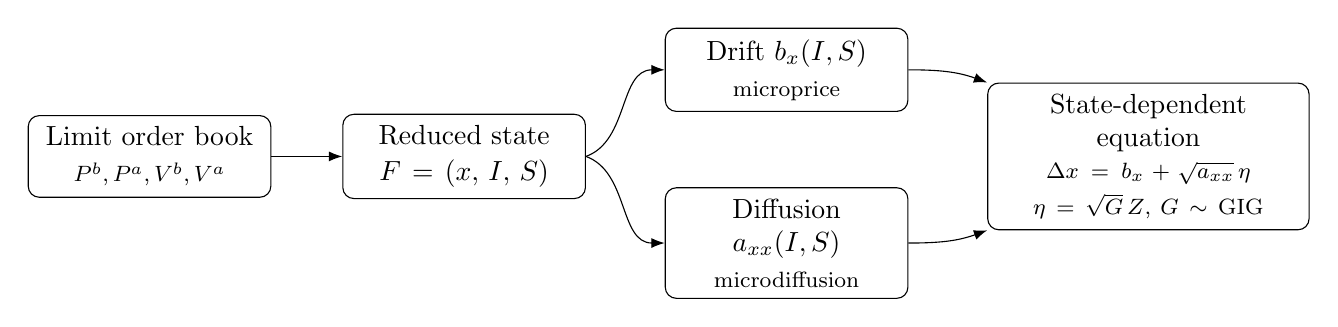
\begin{tikzpicture}[
   >=Latex, node distance=6mm,
   box/.style={draw, rounded corners, align=center, inner sep=4pt, minimum height=9mm,
               text width=28mm},
   widebox/.style={draw, rounded corners, align=center, inner sep=4pt, minimum height=12mm,
               text width=38mm},
   lab/.style={font=\small\itshape, align=center}]
  \node[box] (book) {Limit order book\\[1pt]\footnotesize $P^b,P^a,V^b,V^a$};
  \node[box, right=9mm of book] (state) {Reduced state\\[1pt]$F=(x,\,I,\,S)$};
  \node[box, right=10mm of state, yshift=11mm] (drift) {Drift $b_x(I,S)$\\[1pt]\footnotesize microprice};
  \node[box, right=10mm of state, yshift=-11mm] (diff) {Diffusion $\axx(I,S)$\\[1pt]\footnotesize microdiffusion};
  \node[widebox, right=10mm of drift, yshift=-11mm] (sde)
     {State-dependent equation\\[2pt]\footnotesize $\Delta x=b_x+\sqrt{\axx}\,\eta$\\[1pt]\footnotesize $\eta=\sqrt{G}\,Z$, $G\sim\GIG$};
  \draw[->] (book) -- (state);
  \draw[->] (state.east) to[out=20,in=180] (drift.west);
  \draw[->] (state.east) to[out=-20,in=180] (diff.west);
  \draw[->] (drift.east) to[out=0,in=160] (sde.north west);
  \draw[->] (diff.east) to[out=0,in=200] (sde.south west);
\end{tikzpicture}
\caption{From the order book to a state-dependent stochastic equation for the price.
The reduced state $(x,I,S)$ feeds a conditional drift, the microprice, and a
conditional diffusion; the two assemble into a single equation whose innovation is a
heavy-tailed normal variance mixture.}
\label{fig:schematic}
\end{figure}

\subsection{Reduced order-book state}
\label{sub:state}

We work in \emph{event time}: let $n=0,1,2,\dots$ index consecutive cleaned
level-one book updates. At update $n$ we observe the best bid price $P^b_n$ and the best
ask price $P^a_n$, together with the volumes $V^b_n$ and $V^a_n$ resting at those
two levels. From these we form the mid-price
\begin{equation}
  M_n \;=\; \tfrac{1}{2}\bigl(P^b_n + P^a_n\bigr),
\end{equation}
and three summary coordinates: the \emph{log mid-price displacement}
\begin{equation}
  x_n \;=\; \log\!\frac{M_n}{M_{\mathrm{ref}}},
  \label{eq:x}
\end{equation}
measured relative to a fixed reference level $M_{\mathrm{ref}}$ so that $x_n$ is
dimensionless; the best-level \emph{imbalance}
\begin{equation}
  I_n \;=\; \frac{V^b_n - V^a_n}{V^b_n + V^a_n} \;\in\; [-1,1],
  \label{eq:I}
\end{equation}
which is positive when the bid side is heavier and negative when the ask side is;
and the \emph{relative spread}
\begin{equation}
  S_n \;=\; \frac{P^a_n - P^b_n}{M_n} \;\ge\; 0,
  \label{eq:S}
\end{equation}
the quoted spread expressed as a fraction of the mid. We collect these into the
\emph{reduced state}
\begin{equation}
  F_n \;=\; (x_n,\, I_n,\, S_n) \;\in\; \Real\times[-1,1]\times\Real_{\ge 0}.
  \label{eq:state}
\end{equation}
The qualifier ``reduced'' is deliberate: $F_n$ is a deliberately small summary of
the book, retaining the price level and the two features, imbalance and
spread, that the microprice literature has identified as carrying short-horizon
information, and discarding the remainder of the book (depth beyond the touch, the
full history of order flow, the identities of participants). The part of the book
we retain we call \emph{resolved}; the part we discard we call \emph{unresolved}.
The framework that follows is a disciplined way of describing the next move of the
price using only the resolved state while accounting honestly for the unresolved
remainder.

We denote the one-step (one-update) change of any quantity by $\Delta$; thus
\begin{equation}
  \Delta F_n \;=\; F_{n+1} - F_n,
  \qquad
  \Delta x_n \;=\; x_{n+1} - x_n,
\end{equation}
and $\Delta x_n$ is the one-step log-return of the mid-price, the central quantity
of the paper. The increment is taken per book update, $\Delta n = 1$; the elapsed
clock time between updates, $\Delta\tau_n$, is not used in the primary model and
enters only the cross-clock comparison of Section~\ref{sub:protocols} and
the calendar-time bridge of Appendix~\ref{app:derivations}.

\subsection{Conditional drift and microdiffusion as event-time moments}
\label{sub:moments}

Suppose the state currently takes the value $F_n=f$. There are exactly two
first-order questions one can ask about the next price increment $\Delta x_n$: in which
direction it moves on average, and how widely it is dispersed about that average.
These are the \emph{event-time conditional moments} of the increment. We define the
\emph{conditional drift}
\begin{equation}
  b_x(I,S) \;=\; \E\!\left[\Delta x_n \given I_n=I,\; S_n=S\right],
  \label{eq:drift}
\end{equation}
the one-step conditional mean increment, and the \emph{microdiffusion}
\begin{equation}
  \axx(I,S) \;=\; \Var\!\left(\Delta x_n \given I_n=I,\; S_n=S\right),
  \label{eq:axx-def}
\end{equation}
the one-step conditional variance of the log-return. Both are conditional moments
\emph{per book update}, not calendar-time rates: there is no hidden division by an
interval $\Delta t$, and no $\Delta t$ appears in the primary model. By analogy with
the microprice, which is the book-state conditional drift, we call $\axx(I,S)$ the
\emph{microdiffusion}: the book-state conditional second moment of the next price
increment. The argument $(I,S)$ rather than the full state $(x,I,S)$ is justified
by the closure of Section~\ref{sub:decomp} and the drift restriction of
Section~\ref{sub:drift}: the first two moments of the increment depend on the book
through the imbalance and the spread, not through the price level.

\textbf{Mean-square estimator.} In event time the conditional mean square of the
increment decomposes \emph{exactly}, by the identity $\E[Y^2]=\Var(Y)+(\E Y)^2$ with
$Y=\Delta x_n$:
\begin{equation}
  \E\!\left[(\Delta x_n)^2 \given I_n=I,\; S_n=S\right]
  \;=\; \axx(I,S) \;+\; b_x(I,S)^2 .
  \label{eq:msq}
\end{equation}
This is not an asymptotic statement about a small step $\Delta t$; it is an exact
event-time decomposition. The squared-drift term is negligible here for an
\emph{empirical}, not an asymptotic, reason: the mid-price is close to a martingale at
the one-update horizon, so the fitted $b_x$ is of order $10^{-7}$ in log units while
$\sqrt{\axx}$ is of order $10^{-4}$, making $b_x^2$ smaller than $\axx$ by some six
orders of magnitude. We record the consequence as a proposition.

\begin{proposition}[Mean-square estimator of the microdiffusion]
\label{prop:estimator}
For every state $(I,S)$ the conditional mean square of the one-step log-return
satisfies the exact decomposition \eqref{eq:msq}. Because the fitted drift is
empirically negligible relative to $\sqrt{\axx}$ at the one-update horizon,
\begin{equation}
  \E\!\left[(\Delta x_n)^2 \given I_n=I,\; S_n=S\right]
  \;=\; \axx(I,S)\,\bigl(1 + \delta(I,S)\bigr),
  \qquad |\delta| = b_x^2/\axx \ll 1,
  \label{eq:prop-est}
\end{equation}
so partitioning the data by the state $(I,S)$ and averaging $(\Delta x_n)^2$ within
each part estimates the microdiffusion directly, with no prior estimate of the drift.
We use the centred form $\E[(\Delta x_n-b_x)^2\given I,S]$ where the squared-drift term
matters, in the identification of Section~\ref{sub:identification}.
\end{proposition}

\noindent
We therefore report the microdiffusion as the per-update conditional second moment,
writing the surface
\begin{equation}
  \axx(I,S) \;=\; \E\!\left[(\Delta x_n)^2 \given I_n=I,\; S_n=S\right],
  \label{eq:axx-surface}
\end{equation}
a function of two variables, with the understanding from \eqref{eq:msq} that the
uncentred and centred forms coincide to six significant figures. Because $\axx$ is a
variance \emph{per book update}, it is not automatically comparable across samples
recorded on different clocks; the leading-order conversion to a calendar-time rate is
deferred to Section~\ref{sub:protocols} and Appendix~\ref{app:derivations}.

\subsection{Second-moment closure}
\label{sub:decomp}

For the drift and the microdiffusion to be well-defined functions of the resolved
state $(I,S)$ alone, the first two conditional moments of the next increment must
depend on the full state $F_n=(x_n,I_n,S_n)$ only through $(I_n,S_n)$. We adopt
this, and only this, as the maintained closure.

\begin{assumption}[Second-moment closure]
\label{ass:closure}
The conditional mean and variance of the next event-time price increment depend on the
resolved state only through the imbalance and the spread:
\begin{equation}
  \E\!\left[\Delta x_n \given F_n\right] = b_x(I_n,S_n),
  \qquad
  \Var\!\left(\Delta x_n \given F_n\right) = \axx(I_n,S_n).
  \label{eq:closure}
\end{equation}
\end{assumption}

\noindent
The mean restriction is precisely the paper's hypothesis~(H1), the drift is
effectively two-dimensional in $(I,S)$ (Section~\ref{sub:drift}), and the variance
restriction is its second-moment counterpart, the statement that makes the
microdiffusion well-defined. We therefore present the closure as \emph{H1 extended to
the second moment}, not as a brand-new assumption. It is deliberately weaker than full
distributional closure: the stronger statement
$\mathcal{L}(\Delta x_n\given F_n)=\mathcal{L}(\Delta x_n\given I_n,S_n)$, which would
make the \emph{entire} standardised residual law common across states, is \emph{not}
assumed. That is a tail-model claim, and we assess it empirically as a robustness
diagnostic (Section~\ref{sec:results}) rather than building it into the closure.

Under the second-moment closure every increment splits into a part that is predictable
from the resolved state and a part that is not:
\begin{equation}
  \Delta x_n \;=\; \underbrace{b_x(I_n,S_n)}_{\text{predictable drift}}
  \;+\; \underbrace{\varepsilon_n}_{\text{unresolved fluctuation}},
  \qquad
  \E[\varepsilon_n \given F_n] = 0,
  \qquad
  \E[\varepsilon_n^2 \given F_n] = \axx(I_n,S_n).
  \label{eq:decomp}
\end{equation}
The residual $\varepsilon_n$ has, by construction, zero conditional mean, every
component the state can predict has been placed in the drift, and its conditional
variance is the microdiffusion. The residual is the footprint of the unresolved order
flow; $\axx$ is the modelled statistics of that footprint.
Equation~\eqref{eq:decomp} fixes the first two conditional moments of
$\varepsilon_n$ but says nothing about the shape of its distribution; specifying that
shape is the subject of Sections~\ref{sub:sde}--\ref{sub:innovation} and of
hypothesis~(H3). The closure leads directly to an empirical test: if $\axx$ is
genuinely a function of the state, a surface estimated on one set of days should
reappear on others; if it is sampling noise dressed as structure, it should not. That
transfer test is the empirical heart of the paper and is the content of
hypothesis~(H2).

\subsection{Drift restriction, microprice, and effective two-dimensionality}
\label{sub:drift}

The microprice of \citet{stoikov2018} can be written as the mid-price plus an
adjustment that is a function of the imbalance and the spread,
\begin{equation}
  P^{\mathrm{micro}}_n \;=\; M_n + \phi(I_n, S_n),
  \qquad
  \phi(I,S) \;=\; \E\!\left[\,M_\infty-M_n \given I_n=I, S_n=S\,\right],
  \label{eq:microprice}
\end{equation}
a conditional future displacement (or, in finite-horizon implementations, its
truncated analogue). We are careful not to identify our drift with this object: $b_x(I,S)$
is the \emph{one-step} conditional mean increment of the log mid-price, the drift-side
counterpart of the microprice adjustment, and not literally the Stoikov fixed point
$\phi$. What we test is the structural content shared by both: that the conditional
drift depends on the imbalance and the spread \emph{alone}, and not on the price level
$x$. We state this as the second assumption, an empirical restriction on the drift.

\begin{assumption}[Drift restriction; effective two-dimensionality]
\label{ass:drift}
The conditional drift of the log mid-price does not depend on the price level once
the imbalance and the spread are known:
\begin{equation}
  \E\!\left[\Delta x_n \given x_n, I_n, S_n\right]
  \;=\;
  \E\!\left[\Delta x_n \given I_n, S_n\right].
  \label{eq:drift-restriction}
\end{equation}
\end{assumption}

\noindent
Assumption~\ref{ass:drift} is the formal statement of hypothesis~(H1). It says that,
for the purpose of \emph{steering} the price, predicting the direction of the next
move, the third coordinate $x$ is redundant given $(I,S)$; the drift is
\emph{effectively two-dimensional}. The price level is not thereby discarded from the
model: $x$ is the variable that \emph{diffuses}, and its conditional dispersion is
exactly the surface $\axx(I,S)$ of \eqref{eq:axx-surface}. In the decomposition of
the price dynamics into a mean and a fluctuation, the imbalance and the spread carry
the mean (through $b_x$, equivalently $\phi$) and the price coordinate carries the
fluctuation (through $\axx$). Whereas the microprice literature has developed the
former, the latter is the new content this paper supplies.

\subsection{Event-time stochastic equation}
\label{sub:sde}

The drift $b_x(I,S)$ and the microdiffusion $\axx(I,S)$ are exactly the two ingredients
required to write an equation of motion for the price. Combining them gives the
\emph{event-time stochastic equation}, the formal object of the paper:
\begin{equation}
  \boxed{\;\;
  \Delta x_n \;=\; b_x(I_n,S_n) \;+\; \sqrt{\axx(I_n,S_n)}\;\eta_n,
  \qquad \Delta n = 1,
  \;\;}
  \label{eq:sde}
\end{equation}
where $\eta_n$ is a mean-zero, unit-variance random innovation. In words: at each book
update the price receives a small, state-dependent \emph{pull}, the drift-side
counterpart of the microprice, together with a \emph{random kick} whose typical size is
set by the book state through $\sqrt{\axx(I,S)}$. Equation~\eqref{eq:sde} is to be read
as a \emph{one-step predictive distribution} per book update, not as a discretised
stochastic differential equation: it specifies the conditional law of the next increment
given the state, with $\Delta n=1$. By analogy with derivatives pricing it is a
local-volatility model indexed by the order-book state, a local-volatility surface
parameterised by the imbalance and the spread rather than by strike and maturity, and
this interpretation, together with the continuous-time Gaussian benchmark, is made
precise in Section~\ref{sub:continuous}. The name ``microdiffusion'' is retained: $\axx$
is a conditional second moment, a diffusion coefficient by analogy, independent of the
clock.

By construction, \eqref{eq:sde} reproduces the first two conditional moments of the
price increment: taking the conditional mean recovers $b_x(I,S)$, and taking the
conditional variance recovers $\axx(I,S)$, since $\eta_n$ has unit variance. What is
\emph{not} fixed by construction, and what the data must decide, is the
\emph{distribution} of the innovation $\eta_n$. The remainder of the framework is
about that distribution.

\subsection{Normal variance-mixture innovations}
\label{sub:innovation}

The simplest choice for the innovation is the standard Gaussian, $\eta_n\sim
\Norm(0,1)$, which makes \eqref{eq:sde} a state-dependent Brownian model. We will
find in Section~\ref{sec:results} that this choice reproduces the conditional
variance but not the conditional tails. The natural remedy, which preserves the
calibrated scale while admitting heavier tails, is to give the innovation a
\emph{random variance}. Let
\begin{equation}
  \eta_n \;=\; \sqrt{G_n}\;Z_n,
  \qquad Z_n\sim\Norm(0,1),
  \qquad G_n>0,
  \qquad Z_n \perp G_n,
  \label{eq:mixture}
\end{equation}
where $G_n$ is a positive random variable, independent of the Gaussian draw $Z_n$,
called the \emph{mixing variable}. Conditional on $G_n$ the innovation is Gaussian,
$\eta_n\given G_n \sim \Norm(0,G_n)$, so the marginal law of $\eta_n$ is a continuous
mixture of mean-zero normals with random variance $G_n$, a \emph{normal variance
mixture}, with density
\begin{equation}
  f_\eta(u) \;=\; \int_0^\infty \frac{1}{\sqrt{2\pi g}}\,
  \exp\!\left(-\frac{u^2}{2g}\right) \pi_G(g)\,\dd g,
  \label{eq:mixture-density}
\end{equation}
where $\pi_G$ is the density of $G_n$. Mixing narrow and wide normals in this way
produces a density that is simultaneously more peaked at the centre and heavier in
the tails than any single normal, which is the qualitative shape of standardised
high-frequency returns.
This product-distribution view is close in spirit to \citet{ma2014model}, who model
stock returns as a normal draw scaled by a random volatility and show that
GIGa volatility mixing gives heavy-tailed return laws, with the Student-$t$ arising
as an important special case. Our use of the mixture is conditional rather than
unconditional: the observable book-state scale $\sqrt{\axx(I,S)}$ is removed first,
and the mixture describes the residual innovation that remains.

The moments of $\eta_n$ follow from \eqref{eq:mixture} by independence and the
symmetry of $Z_n$. Since $\E[Z_n]=0$, $\E[Z_n^2]=1$, and $\E[Z_n^4]=3$,
\begin{align}
  \E[\eta_n] &= \E[\sqrt{G_n}]\,\E[Z_n] = 0, \label{eq:mix-mean}\\
  \E[\eta_n^2] &= \E[G_n]\,\E[Z_n^2] = \E[G_n], \label{eq:mix-var}\\
  \E[\eta_n^4] &= \E[G_n^2]\,\E[Z_n^4] = 3\,\E[G_n^2]. \label{eq:mix-fourth}
\end{align}
Two consequences are central. First, by \eqref{eq:mix-var} the variance of the
innovation equals the mean of the mixing variable, so the unit-variance requirement
of \eqref{eq:sde} is exactly the normalisation
\begin{equation}
  \E[G_n]=1.
  \label{eq:mix-normalisation}
\end{equation}
Imposing \eqref{eq:mix-normalisation} guarantees that the entire scale of the move
resides in $\sqrt{\axx(I,S)}$ and none of it leaks into the innovation. Second, with
\eqref{eq:mix-normalisation} in force, the excess kurtosis of the innovation, the
standard scalar measure of tail heaviness, is, from \eqref{eq:mix-var} and
\eqref{eq:mix-fourth},
\begin{equation}
  \kappa(\eta_n)
  \;=\; \frac{\E[\eta_n^4]}{\bigl(\E[\eta_n^2]\bigr)^2} - 3
  \;=\; \frac{3\,\E[G_n^2]}{\bigl(\E[G_n]\bigr)^2} - 3
  \;=\; 3\left(\E[G_n^2]-1\right)
  \;=\; 3\,\Var(G_n).
  \label{eq:kurtosis-identity}
\end{equation}
The identity \eqref{eq:kurtosis-identity} is exact and independent of the particular
mixing family: once the mixing variable is normalised to unit mean, the tail
heaviness of the innovation is governed by a single number, the variance of the
mixing variable. A degenerate mixing variable, $\Var(G_n)=0$, returns the Gaussian
innovation; any dispersion in $G_n$ buys exactly proportional excess kurtosis.

The family of laws obtained as $\pi_G$ ranges over the \emph{Generalized Inverse
Gaussian} ($\GIG$) distributions is the \emph{Generalized Hyperbolic} ($\GH$) family
of \citet{barndorffnielsen1977,barndorffnielsen1997}:
\begin{equation}
  G_n \sim \GIG \quad\Longrightarrow\quad \eta_n = \sqrt{G_n}\,Z_n \sim \GH.
  \label{eq:gig-gh}
\end{equation}
The $\GH$ family is a convenient and interpretable choice for three reasons. It
nests the alternatives:
an inverse-gamma mixing variable yields a Student-$t$ innovation \citep{bollerslev1987}
and a degenerate one the Gaussian, so $\GH$ interpolates between the
exponential-square tail of the normal and the pure power-law tail of the
Student-$t$. Its tails are \emph{semi-heavy}, asymptotically of the form
$|u|^{\lambda-1}\exp(-\alpha|u|)$, a polynomial times an exponential, heavier than
Gaussian but lighter than any power law, so that, unlike a low-degree Student-$t$,
all of its moments are finite, which is required if $\eta_n$ is to be a genuine
unit-variance innovation. And it is the law that arises from precisely the
subordination mechanism, a Gaussian on a random activity clock, that motivates
heavy tails in returns \citep{clark1973}. Throughout this paper we use the
\emph{symmetric, centred, unit-variance} member of the family, fixing the location
to zero, the skewness parameter to zero, and the scale so that \eqref{eq:mix-var}
and \eqref{eq:mix-normalisation} hold; what remains free is then a low-dimensional tail
shape, the index $\lambda$ of the mixing $\GIG$ law together with a single
tail-decay parameter, which in our fits concentrates near the
Normal-Inverse-Gaussian member ($\lambda=-\tfrac12$). The general $\GH$ law additionally carries location, scale, and skewness
parameters, and relaxing the symmetry restriction is noted in
Section~\ref{sec:robustness} as an extension.

\subsection{Identification of scale and shape}
\label{sub:identification}

The model \eqref{eq:sde} with the variance-mixture innovation \eqref{eq:mixture}
factors the centred price move into a product of a state-dependent \emph{scale} and
a heavy-tailed \emph{shape},
\begin{equation}
  \Delta x_n - b_x(I_n,S_n)
  \;=\; \underbrace{\sqrt{\axx(I_n,S_n)}}_{\text{scale}}\;\cdot\;
  \underbrace{\sqrt{G_n}\,Z_n}_{\text{shape}}.
  \label{eq:factorisation}
\end{equation}
It is important to be precise about what \eqref{eq:factorisation} does and does not
identify, because a natural objection is that the two factors might be confounded.
Write $V_n = \axx(I_n,S_n)\,G_n$ for the instantaneous variance of the move. The
decomposition $V_n = \axx(I,S)\cdot G_n$ is rendered \emph{unique} by the two
conditions already imposed: that the scale is a function of the resolved state,
$\axx\in\sigma(I,S)$, and that the mixing variable has unit conditional mean,
$\E[G_n\given I,S]=1$. Under these two conditions,
\begin{equation}
  \axx(I,S) \;=\; \E\!\left[(\Delta x_n-b_x)^2 \given I,S\right],
  \label{eq:axx-identified}
\end{equation}
so the scale is identified as the conditional mean of the squared centred move, the
diffusion surface of \eqref{eq:axx-surface}, and the multiplier $G_n$ is the
unit-mean residual that remains.

The mixing variable itself, however, is \emph{not} directly observable. From
\eqref{eq:factorisation},
\begin{equation}
  \frac{(\Delta x_n - b_x)^2}{\axx(I,S)} \;=\; G_n\,Z_n^2,
  \qquad
  \E\!\left[G_n Z_n^2 \given I,S\right]
  = \E[G_n\given I,S]\,\E[Z_n^2] = 1,
  \label{eq:gz2}
\end{equation}
so a single move reveals only the product $G_n Z_n^2$, never $G_n$ alone: the burst
$G_n$ and the Gaussian draw $Z_n$ cannot be separated within one observation.
Identification is therefore at the level of \emph{conditional means}, as in
\eqref{eq:axx-identified}, and not move by move. This is the precise sense of
hypothesis~(H4): the scale $\axx$ and the shape (the law of $G_n$, equivalently of
$\eta_n$) are distinct objects, each identified, and Section~\ref{sec:results} shows
that each is empirically necessary, the scale carries the state-dependence of the
move's size, while the shape carries its heavy tail, and neither substitutes for the
other.

This scale--innovation architecture is shared with conditional-volatility models,
especially the Student-$t$ GARCH model of \citet{bollerslev1987}. The distinction is
the conditioning set. The conditional variance \eqref{eq:axx-surface} is a function
of the contemporaneous, observable order-book state $(I,S)$, not of the past of the
return series. This difference makes $\axx$ an observable state surface rather than
only a summary of recent volatility.

\subsection{Continuous-time interpretation}
\label{sub:continuous}

The estimated object is the event-time one-step predictive distribution
\eqref{eq:sde}; the continuous-time, local-volatility language is an
\emph{interpretation} and a Gaussian benchmark, not the fitted model. The distinction
is between the formal estimated object and a useful analogy, and it matters because the
heavy-tailed specification does not admit a naive continuous-time form.

In the Gaussian case, $\eta_n\sim\Norm(0,1)$, the equation has the familiar formal Itô
benchmark
\begin{equation}
  dx_t \;=\; b_x(I_t,S_t)\,dt \;+\; \sqrt{\axx(I_t,S_t)}\;dW_t ,
  \label{eq:sde-cont}
\end{equation}
with $W_t$ a standard Brownian motion. Even this is not a closed continuous-time model
unless the joint dynamics of $(I_t,S_t)$ are specified; it is best read as a
\emph{local It\^o-diffusion benchmark conditional on the observed book state}, and it is
the limit invoked by the local-volatility analogy. The name ``microdiffusion'' survives
the event-time reframing: $\axx$ is a conditional second moment, a diffusion coefficient
by analogy, independent of the clock. Only the continuous-time \emph{SDE claim} is
softened; neither the name nor the local-volatility interpretation is dropped.

The heavy-tailed specification is deliberately kept in event time. One cannot obtain a
valid stochastic differential equation merely by replacing $\eta_n$ with
$\sqrt{G_t}\,dW_t$: the latent multiplier would have to be promoted to a positive
adapted stochastic process $G_t$ with its own dynamics,
\begin{equation}
  dx_t \;=\; b_x(I_t,S_t)\,dt \;+\; \sqrt{\axx(I_t,S_t)\,G_t}\;dW_t ,
  \label{eq:gh-sde}
\end{equation}
which is well-defined only after specifying the dynamics of $G_t$ and of the augmented
state $Y_t=(F_t,G_t)$ (a subordination or Barndorff-Nielsen--Shephard construction).
Since this paper estimates a one-step event-time predictive distribution and does not
estimate a continuous-time $G_t$ process, the full continuous-time Generalized
Hyperbolic model is left as future work. The next section tests whether the surface
$\axx(I,S)$ is stable enough to transfer across days and, where the data permit, across
venues.

% ===========================================================================
\section{Data and Methodology}
\label{sec:data}

\subsection{Venues and samples}
\label{sub:venues}

The primary sample is the full cross-section of a single equity venue (denoted QSE),
summarised in Table~\ref{tab:venues}: $41$ instruments observed over the period
5 January 2025 to 30 April 2026 ($216$ trading sessions), for a total of
approximately $4.03$ million level-one updates. This is the sample on which the paper's main estimation, out-of-sample
tests, GARCH comparison, and heavy-tailed validation are run. We also construct two
smaller external samples for appendix robustness checks: three cryptocurrencies
(Bitcoin, Ether, and Cardano) sampled at one-second resolution over 7--19 April
2021, and a five-name U.S.\ equity sample drawn from the LOBSTER reconstruction for
the single trading day 21 June 2012. These samples are useful stress tests of the
state construction, but they are not treated as co-equal evidence because their
sampling clocks, asset universes, and sample lengths differ materially from QSE.

\begin{table}[!htbp]
\centering
\caption{Data sources. ``Obs.'' is the number of level-one observations after
cleaning. QSE is the primary estimation and validation sample. Crypto and LOBSTER
are used only as appendix robustness checks.}
\label{tab:venues}
\small
\begin{tabular}{@{}llrll@{}}
\toprule
Source & Instruments & Obs. & Period & Clock \\
\midrule
QSE (equity) & 41 & $4{,}032{,}350$ & 2025-01-05 to 2026-04-30 & event \\
Crypto & 3 (BTC, ETH, ADA) & $3{,}089{,}036$ & 2021-04-07 to 2021-04-19 & 1 second \\
LOBSTER (U.S.\ equity) & 5 & $2{,}110{,}860$ & 2012-06-21 (single day) & event \\
\bottomrule
\end{tabular}
\end{table}

For each instrument we retain only well-formed level-one records (positive,
finite mid-price and best-level sizes) and discard crossed or empty books. Two
caveats apply to the robustness samples and are carried through the analysis. The
cryptocurrency market trades continuously, so its ``sessions'' are arbitrary
calendar-day partitions of a single uninterrupted tape rather than exchange
sessions; and Cardano is a low-priced, coarse-tick instrument whose price moves in
a small number of discrete increments, so it is not a clean liquidity analogue of
Bitcoin or Ether. The single-day LOBSTER sample is sufficient to estimate the
diffusion surface cross-sectionally but, having only one day, does not permit a
cross-\emph{day} transfer test; we therefore use it as a consistency check rather
than as a validation sample.

\paragraph{Provenance and scope.}
The QSE sample is reconstructed from the venue's level-one message feed: for each instrument
and trading session we replay the time-stamped best-bid/best-ask quote and size messages and
record the prevailing top of book at each update, retaining only regular continuous-trading
updates with a positive, finite mid-price and positive best-level sizes and discarding
opening- and closing-auction states, halts, and crossed or empty books. The state variables
$(I,S)$ and the increment $\Delta x$ are computed from this reconstructed top of book; no
depth beyond the touch and no trade or participant information enters the analysis. The venue
is a single frontier-market exchange with on the order of fifty listed names, so the $41$-name
sample is effectively the whole market rather than a draw from a broad universe; it is a
thin, wide-spread, coarse-tick market. We are explicit about this throughout: the structural
claims are demonstrated on QSE and replicated where the external samples permit
(Appendix~\ref{app:external}), and we do not assert that the specific numerical surface
generalises unchanged to deep, fine-tick major-market books, only that the construction, the
state-dependence, and the heavy-tailed innovation recur. To support replication we will
release the estimation and analysis code and the processed, instrument-anonymised
state--increment series on which every reported number is computed; the raw exchange feed is
subject to the venue's redistribution terms.

\subsection{Descriptive statistics}
\label{sub:descriptive}
Table~\ref{tab:descr-qse} reports per-instrument summary statistics, the
distributions of the relative spread, the best-level imbalance, the absolute one-step
return, and the top-of-book depth, for the 41 QSE instruments. The $4.03$ million updates
are spread across $1{,}588$ instrument-sessions (not every name trades every day), so the median
session carries $2{,}172$ updates, with a $10$th--$90$th percentile range of
$1{,}598$--$3{,}917$ and a maximum of $17{,}369$; no session falls below one hundred updates.
The thinnest \emph{instruments}, however, a handful contributing only a few thousand updates
in total over the sample, populate the $30$-cell grid sparsely, which is why we impose a
minimum cell count and read their far-tail estimates with the caution noted in
Section~\ref{sec:robustness}. Descriptive statistics for the external robustness samples are
reported in Appendix~\ref{app:external}.
\input{sections/desc_qse}
\FloatBarrier

\subsection{State construction and binning}
\label{sub:binning}

For each instrument we construct the reduced state of Section~\ref{sub:state} at
every update and form the one-step log-return $\Delta x_n$. To estimate the
conditional moments \eqref{eq:axx-surface} non-parametrically we partition the
two-dimensional state $(I,S)$ into a grid: the imbalance $I\in[-1,1]$ into
$N_I=10$ equal-width bins, and the relative spread $S$ into $M_S=3$ terciles whose
cut-points are the empirical $\tfrac13$ and $\tfrac23$ quantiles of $S$ estimated
on the training portion of each instrument. This yields up to $N_I\times M_S=30$
state cells per instrument, each a distinct book configuration; we retain a cell
for estimation only if it contains at least $50$ observations. Within each cell we
estimate the per-step drift $b_x$ and diffusion $\axx$ as the sample mean and
sample mean-square of $\Delta x_n$, following Proposition~\ref{prop:estimator}.

\subsection{Estimation and out-of-sample protocols}
\label{sub:protocols}

All structural claims are tested out of sample. For each instrument we order its
sessions chronologically and assign the first $60\%$ to a training set and the
final $40\%$ to a held-out test set; nothing estimated on the training set is
re-estimated on the test set.\footnote{In particular, the conditional moments $b_x$ and
$\axx$, the spread tercile cut-points, and every innovation-law parameter used to
standardise or score a held-out observation are estimated on the training partition only;
no test-set quantity enters the standardisation. We verified this directly in the estimation
code.} We use four protocols.
\begin{enumerate}
  \item \emph{Cross-day transfer of the diffusion surface.} We estimate $\axx(I,S)$
  on the training days and, independently, the realised cell mean-square on the test
  days, and measure their agreement across cells by the Spearman rank correlation.
  A genuine state function reproduces its shape out of sample; to fix the null we
  also compute the same statistic after randomly permuting the cell labels (a
  \emph{shuffled placebo}), which breaks the link between state and outcome.
  \item \emph{Split-half reliability.} To measure how much of the cross-cell
  ordering is reproducible signal rather than estimation noise, we split the
  training sessions into two disjoint blocks, estimate $\axx$ on each, and correlate
  the two estimates across cells.
  \item \emph{Innovation fitting and out-of-sample tail validation.} We fit the
  symmetric Generalized Hyperbolic innovation by maximum likelihood to the pooled
  standardised residuals $z_n=(\Delta x_n - b_x)/\sqrt{\axx}$. To validate the
  fitted tail law out of sample we split the held-out residuals into two disjoint
  temporal blocks, fit the law on one, and evaluate it on the other, scoring by the
  out-of-sample mean log-likelihood gain over the best Gaussian and by the predicted
  versus realised tail-exceedance frequencies.
  \item \emph{Uncertainty quantification.} We report bootstrap confidence intervals
  (resampling the unit of analysis, which is the instrument or the cell as
  appropriate) and, where a sharper null is informative, permutation tests.
\end{enumerate}

\emph{Cross-clock comparability.} Because the model is written in event time, the
microdiffusion $\axx(I,S)$ is a variance \emph{per book update}, not per unit of calendar
time. Estimates are therefore not automatically comparable across samples recorded on
different clocks: the primary QSE analysis is on the event clock, the crypto appendix is
on a one-second clock, and the LOBSTER probe is event-clock on a single day. We keep
structural claims within each clock, and where a cross-venue magnitude comparison is
needed we convert the event-time variance to a calendar-time rate using the leading-order
bridge $a^{\mathrm{cal}}_{xx}(I,S)\approx a^{\mathrm{event}}_{xx}(I,S)/\E[\Delta\tau_n\mid
I,S]$ derived in Appendix~\ref{app:derivations}, where $\Delta\tau_n$ is the elapsed clock
time between updates. The bridge ignores activity clustering and is used only for
external-sample comparability; it does not enter the primary QSE results.

% ===========================================================================
\section{Empirical Results}
\label{sec:results}

We present the results in the order of the framework: the drift restriction (H1,
Section~\ref{sub:res-drift}); the diffusion surface and its transfer (H2,
Section~\ref{sub:res-axx}); the state-dependent equation under a Gaussian
innovation (H3, first part, Section~\ref{sub:res-gauss}); the heavy-tailed
innovation and its out-of-sample validation (H3, second part,
Sections~\ref{sub:res-gh}--\ref{sub:res-oos}); and the separate identification of
scale and shape (H4, Section~\ref{sub:res-ident}). Throughout, QSE is the estimation
and validation sample unless stated otherwise.

\subsection{Effective two-dimensionality of the drift (H1)}
\label{sub:res-drift}

We first test Assumption~\ref{ass:drift}: that the conditional drift of the price
depends on the imbalance and the spread but not on the price level. Operationally we
compare two out-of-sample predictors of the next log-return: a two-dimensional model
that conditions on $(I,S)$ alone, and a three-dimensional model that adds the price
level $x$. If the level carries genuine additional information about the drift, the
three-dimensional model should predict better out of sample; under
Assumption~\ref{ass:drift} it should not.

Across $1{,}547$ out-of-sample instrument-period pairs, adding the price level does not
improve prediction and slightly degrades it. The out-of-sample coefficient of
determination falls from $R^2_{2\mathrm D}=0.0072$ for the $(I,S)$ model to
$R^2_{3\mathrm D}=-0.0102$ for the $(x,I,S)$ model, a change of
$\Delta R^2 = -0.0174$ with a $95\%$ bootstrap interval of $[-0.0319,\,-0.0075]$
that excludes zero; the directional hit-rate likewise falls from $0.564$ to $0.550$
($\Delta = -0.0137$, $95\%$ CI $[-0.0158,\,-0.0118]$). The absolute predictability is
small in both cases, as expected for one-step high-frequency returns of a
near-martingale, the per-cell mean drift $b_x$ is of order $10^{-7}$ in log units,
economically negligible, but the comparison is unambiguous: the price level adds
nothing to the drift and, through overfitting, marginally detracts from it.
Assumption~\ref{ass:drift} is supported, and the third state coordinate is freed to
play its role as the variable that diffuses.

\begin{figure}[!htbp]
\centering
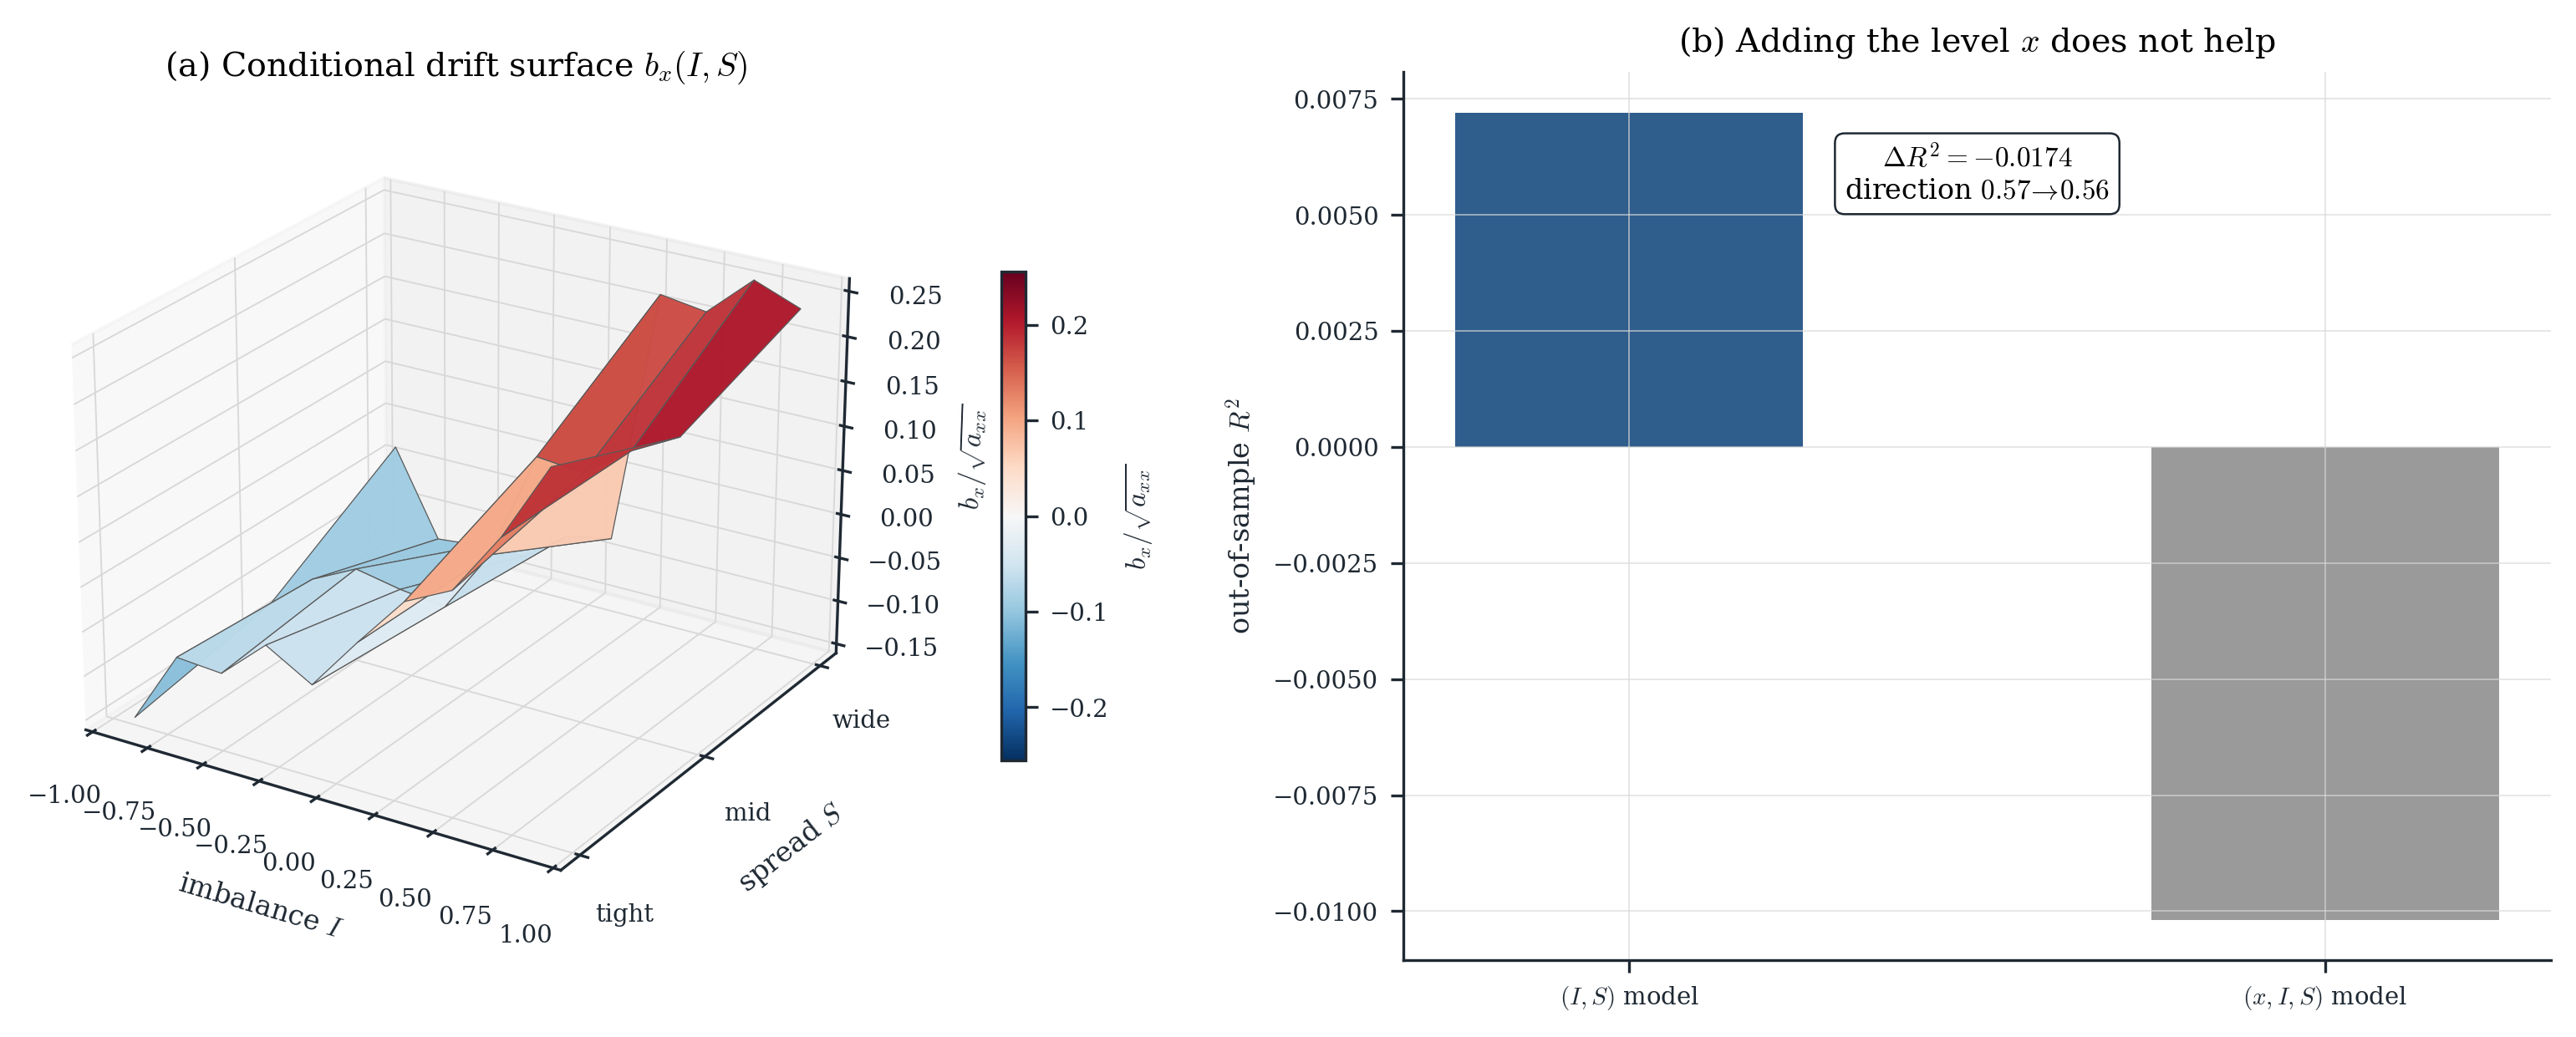
\includegraphics[width=\linewidth]{fig_drift_surface.png}
\caption{The conditional drift is effectively two-dimensional in $(I,S)$. Panel~(a):
the estimated conditional drift $b_x(I,S)$, in units of the local typical move
$\sqrt{\axx}$, averaged across instruments over the imbalance--spread grid; it varies
systematically with the imbalance (positive when the bid is heavier) and is the
empirical content of the microprice. Panel~(b): out-of-sample $R^2$ of the $(I,S)$
model and of the $(x,I,S)$ model; adding the price level $x$ does not improve the
prediction ($\Delta R^2=-0.0174$), supporting Assumption~\ref{ass:drift}.}
\label{fig:drift}
\end{figure}
\FloatBarrier

\subsection{Out-of-sample transfer of the microdiffusion surface (H2)}
\label{sub:res-axx}

The microdiffusion $\axx(I,S)$ varies strongly across book states:
within a typical instrument the surface spans roughly an order of magnitude from its
calmest to its most active cell, and considerably more for thinly traded names. This
variation is economically intuitive: a tight, balanced book should not have the same
short-horizon price dispersion as a wide or one-sided book. The central question is
whether the pattern is stable, or whether it is only a finite-sample picture drawn
from noisy squared returns. Hypothesis~(H2) asserts stability, and the data provide
strong support for it.

Estimating $\axx(I,S)$ on the training days and comparing it, cell by cell, with the
realised cell mean-square on the disjoint test days gives a joint $(I,S)$ transfer
rank correlation of $0.477$ ($95\%$ instrument-clustered bootstrap interval
$[0.395,\,0.561]$; $[0.461,\,0.493]$ under i.i.d.\ resampling), positive for $89.6\%$ of the $1{,}398$ instrument-pairs. The shuffled placebo,
which destroys the link between state and outcome, gives $-0.000$
($[-0.014,\,0.013]$), consistent with no transferable state information. Decomposing
the surface shows
that the spread axis carries most of the transferable structure (spread-only transfer
$0.692$) and the imbalance axis less (imbalance-only $0.155$), with a smaller
interaction term ($0.104$). A complementary split-half analysis, estimating the
surface on two disjoint training blocks and correlating the two, gives a rank
reliability of $0.948$, indicating that the cross-cell ordering of the diffusion is
almost entirely reproducible signal rather than noise.

We are careful to separate two distinct claims. The transfer result establishes that
$\axx(I,S)$ is a \emph{structurally stable function of the state}: it is the same
surface from one set of days to the next. It does \emph{not} claim that conditioning
on the exact state is a superior one-step \emph{forecast} of the next squared return:
relative to a single per-instrument variance, the state-conditional variance adds
essentially nothing as a point forecast (an out-of-sample skill of $-0.0032$,
indistinguishable from zero). Both halves are true simultaneously, and we report them
together: the surface is real and transferable, yet it is a modest one-step
size-forecaster. It is the former property, structural transferability, that
justifies using $\axx(I,S)$ as the diffusion coefficient in the stochastic model
below.

\begin{figure}[!htbp]
\centering
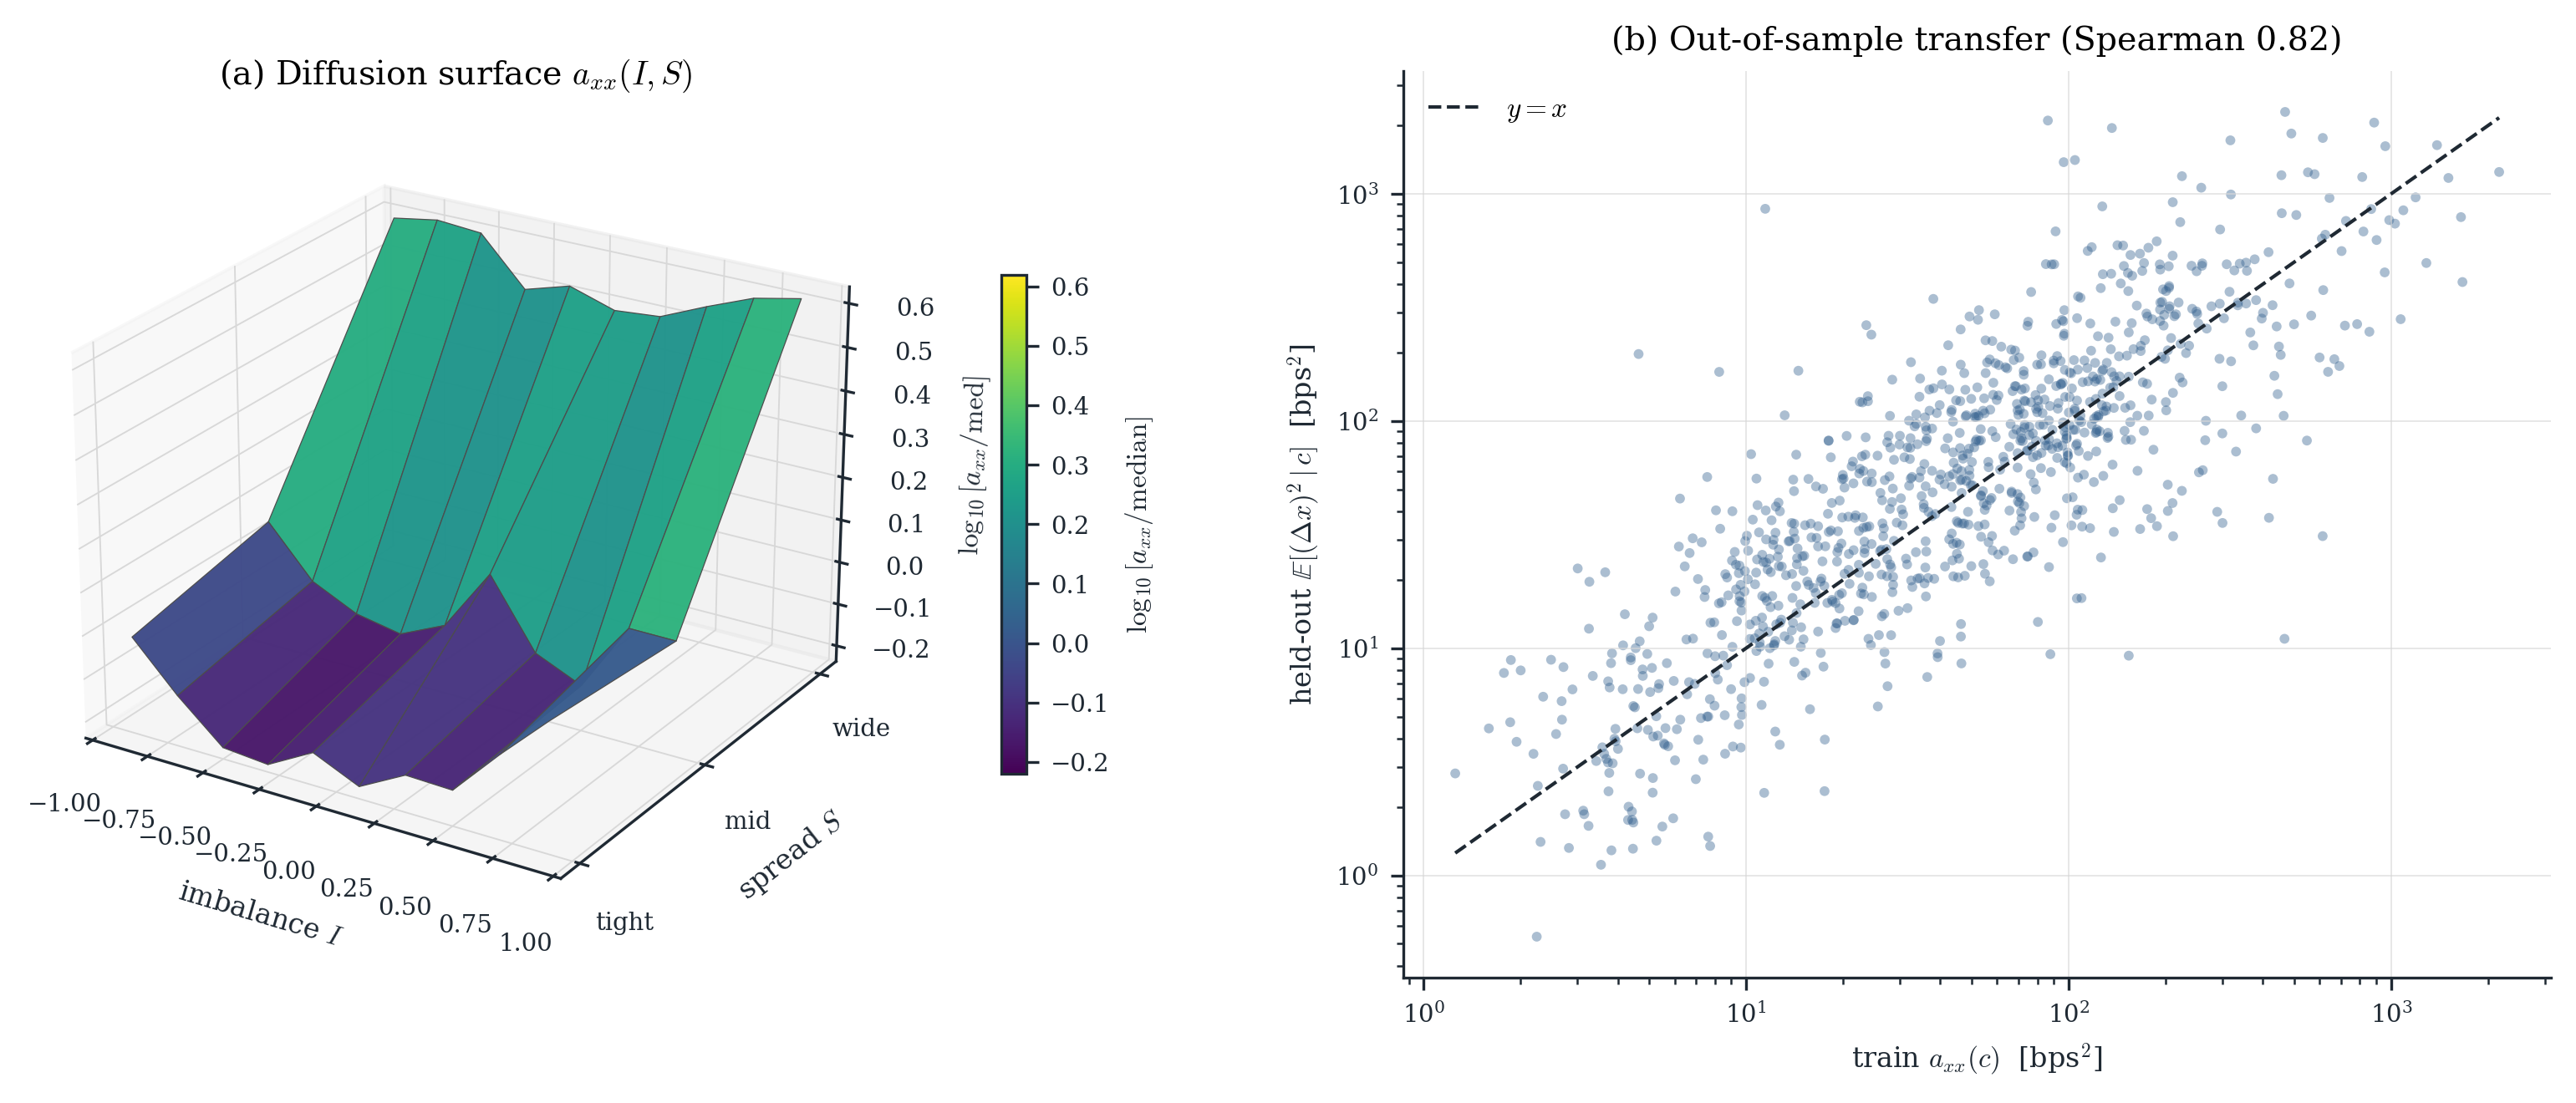
\includegraphics[width=\linewidth]{fig_axx_surface.png}
\caption{The microdiffusion surface $\axx(I,S)$ and its out-of-sample transfer. Panel~(a):
the estimated microdiffusion over the imbalance--spread grid, shown relative to each
instrument's median and on a base-ten logarithmic colour scale; the conditional
variance of price moves rises sharply toward wide spreads and varies with imbalance.
Panel~(b): the out-of-sample calibration scatter of the training $\axx$ against the
held-out realised cell mean-square, pooled across instruments and cells (rank
correlation $0.82$). The headline \emph{within-instrument} transfer reported in the
text, which controls for the instrument-level scale and is compared against a shuffled
placebo, is $0.48$ (placebo $0.00$).}
\label{fig:axx}
\end{figure}

The surface transfers not only across days within an instrument but \emph{across
instruments}, and this is the property that most sharply distinguishes it from a
return-history variance model. In a leave-one-instrument-out exercise we estimate the
shape of the diffusion surface over $(I,S)$ on all but one instrument and apply it to the
held-out instrument. We still grant the held-out instrument one scalar calibration, its
overall volatility level, so this is a minimal target-calibration test rather than a
zero-data listing-day forecast. Conditional on that one scalar, however, the entire
state-conditional shape is borrowed from \emph{other} instruments. The borrowed surface
predicts the held-out instrument's realised per-state variance at a cross-instrument rank
correlation of $0.81$ (Figure~\ref{fig:transfer}, panel a), essentially the same as the
within-instrument figure. As a forecaster it loses almost nothing relative to the
instrument's own surface (a mean out-of-sample predictive log-likelihood difference of
only $-0.012$ per observation) and improves on the \emph{one-scalar floor}, a constant
variance forecast using the same overall volatility level, by $+0.10$ per observation,
for $78\%$ of instruments (Figure~\ref{fig:transfer}, panel b).

The contrast with a GARCH forecast is structural, not a matter of degree. The diffusion
surface is a cross-sectional map from the observable book state to the conditional
variance, shared across instruments; a GARCH model is a within-series recursion whose
forecast is a function of the instrument's own past returns. In a genuine cold start a
return-history recursion has no past returns from which to infer a dynamic variance path.
The experiment here asks the narrower, testable question: once a single volatility level
is known for the target instrument, can the \emph{shape} of the state-dependent surface be
borrowed cross-sectionally? The answer is yes. The book-state shape, unlike a return
history, is portable, and that portability, rather than any advantage in one-step
forecasting accuracy, is the practical content of the surface's structural stability.

\begin{figure}[!htbp]
\centering
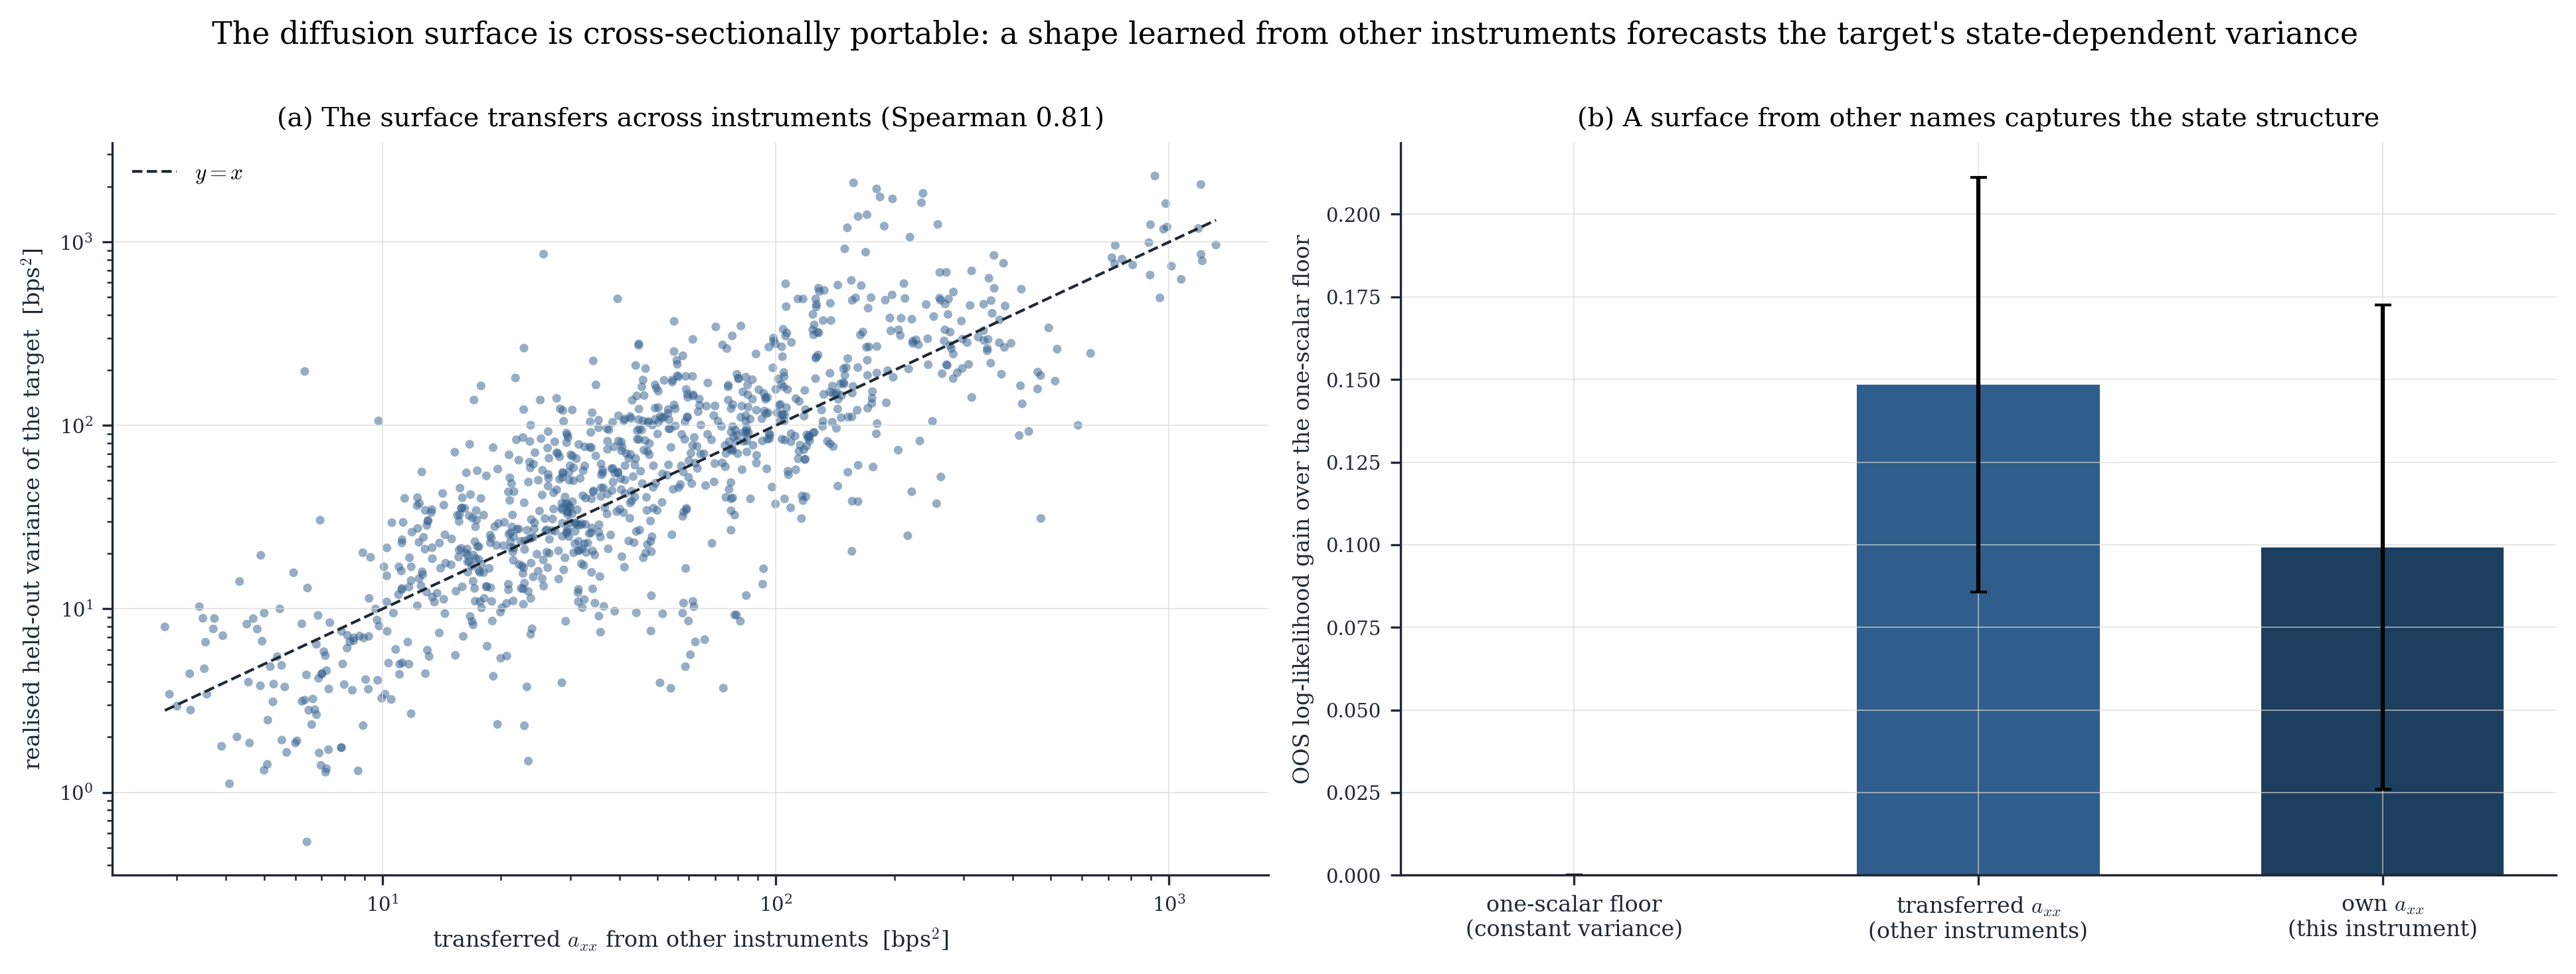
\includegraphics[width=\linewidth]{fig_transfer_coldstart.png}
\caption{The diffusion surface is cross-sectionally portable. Panel~(a): a leave-one-%
instrument-out transfer, the surface estimated on \emph{all other} instruments,
rescaled only by the held-out instrument's overall volatility, against that instrument's
realised held-out per-state variance (cross-instrument rank correlation $0.81$). Panel~(b):
out-of-sample predictive log-likelihood gain over the one-scalar floor, a constant
variance forecast using the same target volatility level. A surface borrowed entirely from
other instruments captures almost all of the gain achieved by the instrument's own
surface; a pure return-history recursion does not supply this cross-sectional state shape
without the target's own return history.}
\label{fig:transfer}
\end{figure}
\FloatBarrier

\subsubsection*{Tick-grid control for the imbalance effect}
\label{sub:res-tick}

A mechanical alternative must be ruled out before the surface can be called a structural
object. In a coarse-tick market a wider quoted spread is a sparser book, and a sparser book
permits larger mid-price moves when the touch updates; since the spread axis carries most of
the surface's transferable level structure, that part of the surface could in principle be a
restatement of the tick grid. We therefore separate two questions that the raw transfer
conflates: (i) does the imbalance still \emph{move} the conditional variance once the tick
mechanics are held fixed, and (ii) does that imbalance structure \emph{transfer} out of
sample? We recover the tick size separately for each instrument from its decimal quote
grid, in the QSE sample this gives instrument-specific ticks of either QAR~$0.001$ or
QAR~$0.010$, then re-express every move and the spread in ticks, and
\emph{stratify by spread-in-ticks}
($1,2,3,\ge 4$), so that within a stratum the mechanical spread--move relationship is held
constant by construction.

On the first question the answer is unambiguous, and it defeats the mechanical alternative.
Holding spread-in-ticks fixed, imbalance continues to move the conditional variance: a
shape-agnostic Kruskal--Wallis test across imbalance bins within a stratum is significant at
the $5\%$ level in $90\%$ of (instrument, stratum) cells, and in $100\%$ of cells at the
tightest ($1$-tick) and widest ($\ge 4$-tick) spreads. The effect is \emph{symmetric}, not
signed: a monotone rank correlation of variance against $I$ is weak ($+0.07$ in the $1$-tick
stratum), but the correlation against $\lvert I\rvert$ is strong ($+0.45$), and extreme
imbalance of either sign carries about \emph{twice} the conditional variance of a balanced
book ($\axx$ ratio $1.98$ in tight books). This is a genuinely new structural fact and not a
tick artifact: it reveals a \emph{second-moment} role for imbalance that is distinct from its
established \emph{first-moment} role in the microprice. The \emph{sign} of the imbalance steers
the conditional mean, the content of the microprice, while the \emph{magnitude} of the
imbalance, on either side, inflates the conditional variance. Order-book imbalance thus enters
both moments of the price increment, through different functionals.

The second question, whether that imbalance structure also transfers across days, calls for a
careful choice of statistic, because the obvious pooled transfer is the wrong one. Pooling
$\axx$ across all instruments and strata gives a high rank correlation ($0.84$), but that
number is biased upward: it reintroduces exactly the instrument-level and spread-level
differences that the stratification was meant to remove, and so it measures the level
structure, not the imbalance shape. The honest object is the transfer of the imbalance shape
\emph{after} removing each instrument$\times$stratum level: pooling the
within-cell log-demeaned $\axx$, the train-to-test rank correlation is only $0.04$ (the
per-stratum within-instrument transfers average $+0.04$, ranging from $-0.07$ to $+0.16$,
and are mixed in sign across strata). The
imbalance modulation of the diffusion is therefore real and contemporaneously strong but
essentially \emph{not reproducible} day-to-day at the within-stratum level. The honest summary is this:
the diffusion surface is not reducible to the tick grid, but its transferable level structure
is mainly carried by the spread; imbalance contributes a real, symmetric, state-dependent
modulation of the variance, but this modulation does not itself transfer across days
(Figure~\ref{fig:tickcontrol}). The paper's transferability claim therefore rests on the
cross-day and cross-instrument transfer of the full surface reported above, of which the
tick-controlled imbalance shape is the weaker component.

\begin{figure}[!htbp]
\centering
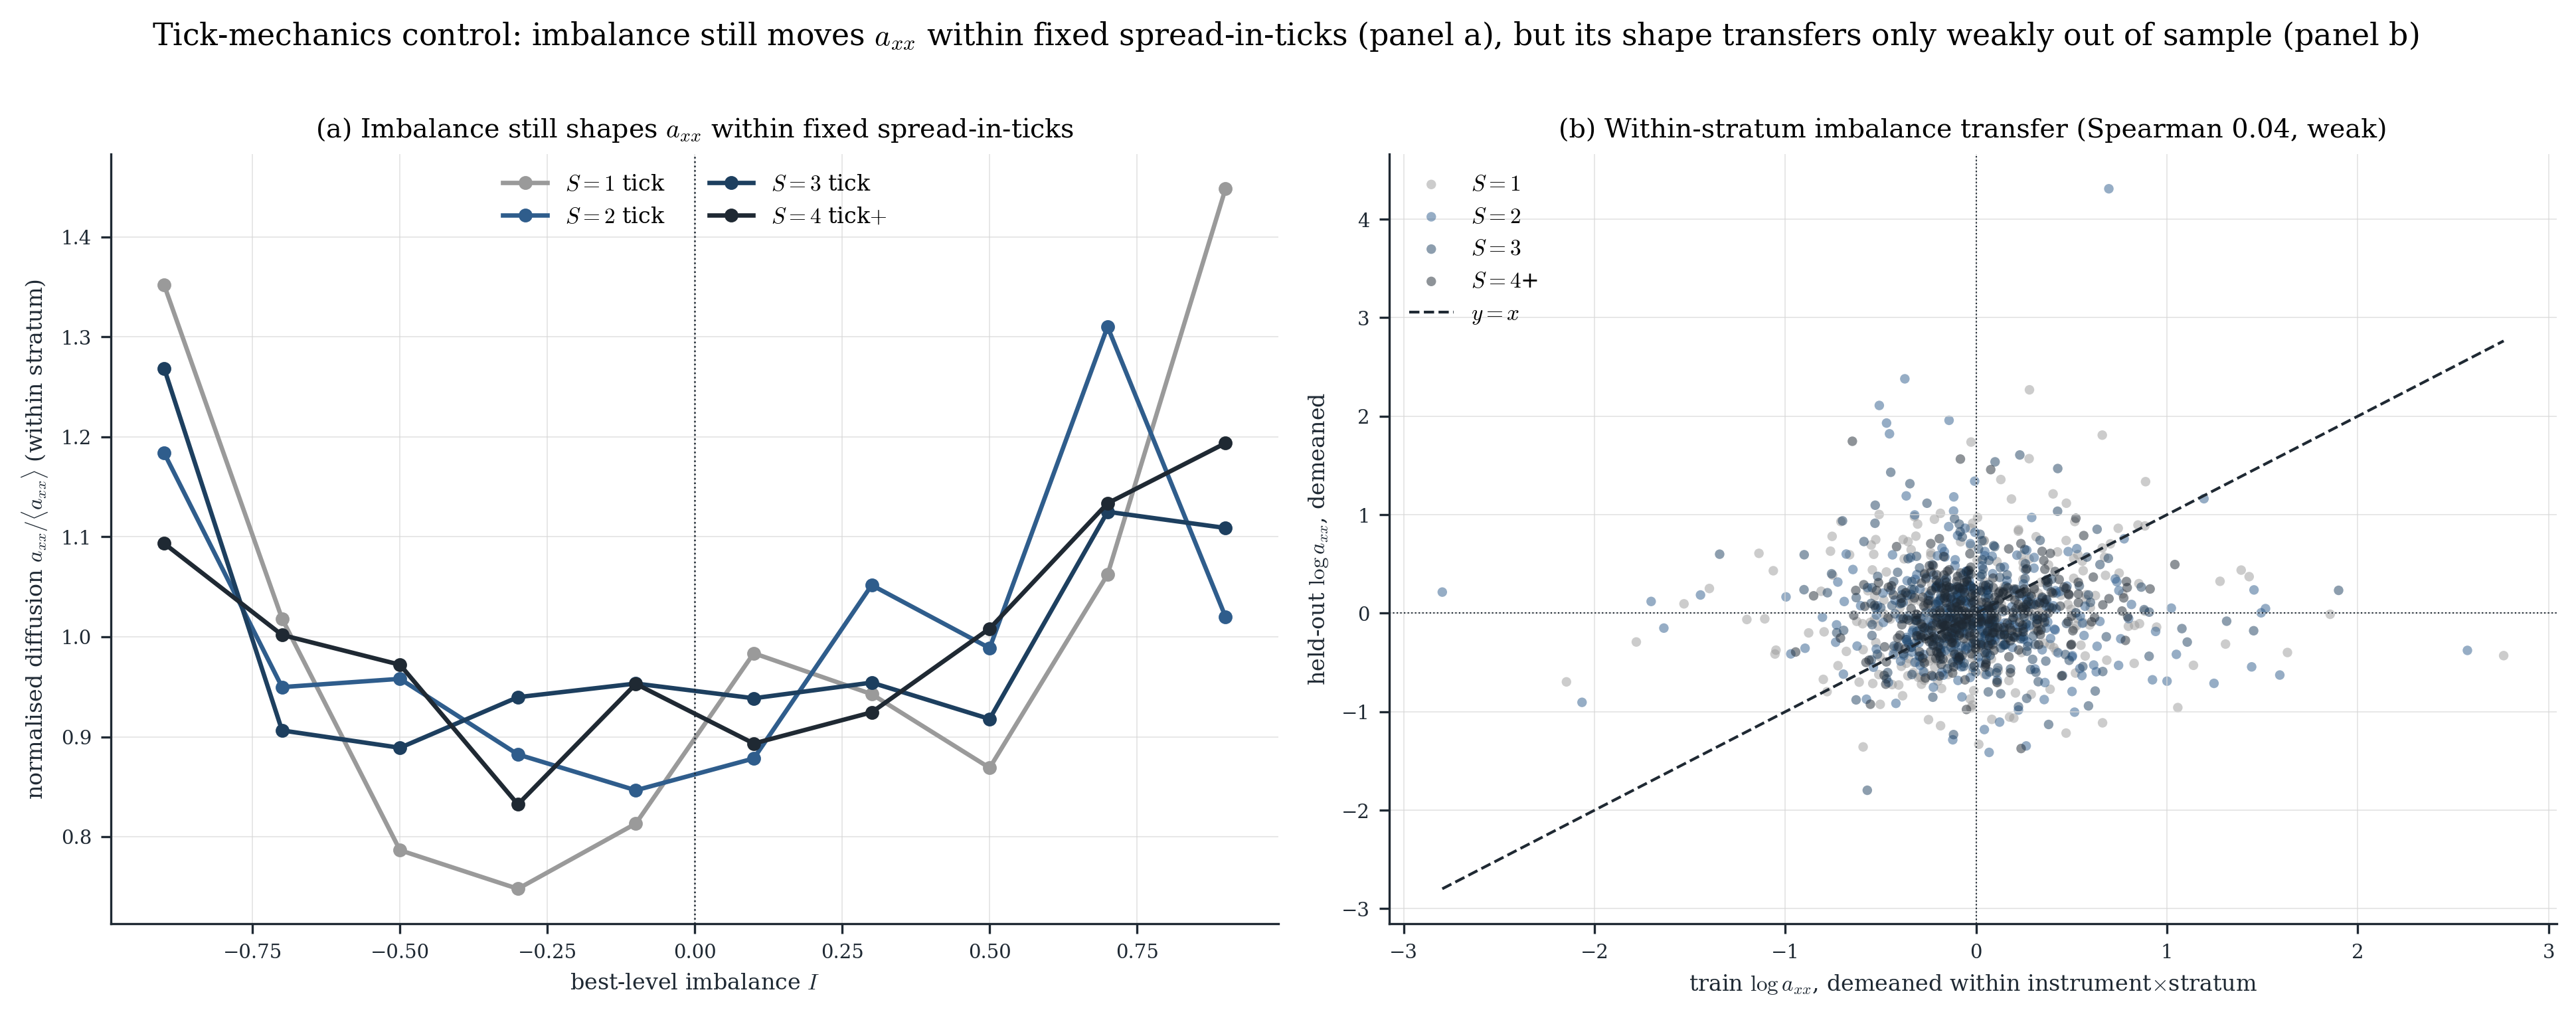
\includegraphics[width=\linewidth]{fig_tick_control.png}
\caption{Tick-mechanics control. Holding spread-in-ticks fixed removes the mechanical
spread--move relationship by construction. Panel~(a): the normalised diffusion
$\axx/\langle\axx\rangle$ against imbalance $I$, one curve per spread-in-ticks stratum; within
every stratum the variance rises for extreme imbalance of \emph{either} sign, a symmetric,
U-shaped effect that a signed correlation would miss, and that is not a tick artifact.
Panel~(b): the honest within-stratum transfer of the imbalance shape, train against held-out
$\log\axx$ after demeaning within each instrument$\times$stratum, so that only the imbalance
shape remains (rank correlation $0.04$, essentially zero). Imbalance robustly \emph{moves} the conditional
variance within fixed spread-in-ticks, but its shape does not reproduce out of sample;
the transferable level structure is carried by the spread axis.}
\label{fig:tickcontrol}
\end{figure}
\FloatBarrier

\subsection{Gaussian innovation benchmark and tail miscalibration (H3a)}
\label{sub:res-gauss}

Having established both ingredients, the drift $b_x(I,S)$ and the diffusion
$\axx(I,S)$, we assemble the state-dependent equation \eqref{eq:sde} and confront
it with held-out data under the Gaussian innovation $\eta_n\sim\Norm(0,1)$. This is
the simplest possible version of the model: the book state determines the local
mean and local variance, and the remaining shock is assumed normal. The model
captures the \emph{scale} of moves well out of sample. The training diffusion
$\axx$ predicts the realised held-out cell
mean-square with a rank correlation of $0.82$ (Figure~\ref{fig:prototype}, variance
calibration). Standardising each move by its cell's diffusion,
$z_n=(\Delta x_n-b_x)/\sqrt{\axx}$, yields residuals with a standard deviation of
$1.29$, close to the target of one; conditioning on the state removes the
heteroskedasticity only slightly better than a single global variance does (per-cell
standard deviation of $z$ of $1.19\pm0.58$ for the state model), consistent with the
modest forecasting skill noted above.

The \emph{shape}, however, is not Gaussian. The standardised residuals are far heavier-tailed
than the unit-variance Gaussian innovation the model assumes: the probability that
$|z_n|$ exceeds three local standard deviations is $0.0264$, against the standard-normal
value of $0.0027$, about ten times too many, and the probability of exceeding five
local standard deviations is $0.0091$, against a standard-normal value of
$5.7\times10^{-7}$. (These reference figures are those of the ideal $\Norm(0,1)$
innovation; the ``best-fit Gaussian'' row of Table~\ref{tab:tails} instead refits the
Gaussian to the residuals' empirical width, which inflates its moderate-range
probabilities while leaving the far-tail collapse intact.) The excess
kurtosis of the residuals is large and is driven by a small number of extreme moves.
The implication is precise. The conditional variance captures the local scale, but
the Gaussian innovation badly understates the conditional tails. The main remaining
misspecification is therefore the distributional shape of the innovation $\eta_n$,
rather than the state-dependent scale itself.

\begin{figure}[!htbp]
\centering
\includegraphics[width=\linewidth]{sde_prototype.png}
\caption{The state-dependent equation under a Gaussian innovation, on held-out data.
The conditional variance is well calibrated out of sample (variance calibration,
rank correlation $0.82$) and conditioning removes heteroskedasticity, but the
standardised residuals remain heavy-tailed, the model has well-calibrated scale but
misspecified tails.}
\label{fig:prototype}
\end{figure}
\FloatBarrier

\subsection{Generalized Hyperbolic innovations and tail fit (H3b)}
\label{sub:res-gh}

The preceding subsection tells us what needs to change. We keep the same drift and
diffusion surface, but replace the Gaussian innovation by the normal variance
mixture of Section~\ref{sub:innovation}. We compare, at the common width of the residuals, the
best-fit Gaussian, two Student-$t$ specifications (one by maximum likelihood, one by
kurtosis matching), and the symmetric Generalized Hyperbolic fitted by maximum
likelihood. Table~\ref{tab:tails} reports the tail-exceedance probabilities
$P(|z|>k)$.

\begin{table}[!htbp]
\centering
\caption{Tail-exceedance probabilities $P(|z|>k)$ of the standardised residuals
(QSE, pooled, $n=1{,}596{,}538$), compared with candidate innovation laws fitted at the
residuals' width. The ``best-fit Gaussian'' refits the Gaussian at the empirical residual
width; it is not the ideal $\mathcal{N}(0,1)$. The Gaussian collapses in the far tail;
the Generalized Hyperbolic closely matches the empirical exceedance profile over this range.}
\label{tab:tails}
\small
\begin{tabular}{@{}lrrrrr@{}}
\toprule
 & $k{=}2$ & $k{=}3$ & $k{=}4$ & $k{=}5$ & $k{=}6$ \\
\midrule
Data (empirical)            & $5.8\times10^{-2}$ & $2.6\times10^{-2}$ & $1.5\times10^{-2}$ & $9.2\times10^{-3}$ & $6.0\times10^{-3}$ \\
Best-fit Gaussian           & $1.2\times10^{-1}$ & $2.0\times10^{-2}$ & $1.9\times10^{-3}$ & $1.0\times10^{-4}$ & $3.0\times10^{-6}$ \\
Student-$t$ (kurtosis, $\nu=4.30$)& $9.6\times10^{-2}$ & $3.0\times10^{-2}$ & $1.1\times10^{-2}$ & $4.9\times10^{-3}$ & $2.4\times10^{-3}$ \\
Generalized Hyperbolic (ML) & $6.3\times10^{-2}$ & $3.1\times10^{-2}$ & $1.7\times10^{-2}$ & $9.8\times10^{-3}$ & $6.0\times10^{-3}$ \\
\bottomrule
\end{tabular}
\par\smallskip
{\footnotesize\flushleft The maximum-likelihood Student-$t$ (not shown) is pulled to
$\hat{\nu}=1.56$, below two (no finite variance); it is excluded as a candidate
innovation law.}
\end{table}

The pattern is clear and is shown in Figure~\ref{fig:heavytail}. The Gaussian, forced
to the correct width, over-populates the moderate range and then collapses in the
tail, understating the frequency of five-standard-deviation moves by more than two
orders of magnitude. The maximum-likelihood Student-$t$ is dragged by the extreme
observations to a degrees-of-freedom parameter $\nu=1.56$, below the value of two at
which the variance ceases to exist, so it cannot serve as a finite-variance
innovation at all, and it over-states the far tail; the kurtosis-matched Student-$t$
($\nu=4.30$) has finite variance but now under-states it. The Generalized Hyperbolic
matches the data closely across the range from $k=2$ to $k=6$, while retaining finite
moments. Its fitted shape sits at the Normal-Inverse-Gaussian corner of the family.
Finally, simulating the equation with the fitted Generalized Hyperbolic kick and the
real sequence of state scales closely reproduces the empirical frequency of large moves,
whereas the Gaussian-driven simulation produces essentially no moves beyond five
local standard deviations (Figure~\ref{fig:ghsim}, Appendix~\ref{app:figures}).

\begin{figure}[!htbp]
\centering
\includegraphics[width=\linewidth]{sde_heavytail.png}
\caption{Density (left) and tail exceedance (right) of the standardised residuals,
with the best-fit Gaussian, Student-$t$, and Generalized Hyperbolic innovations at
the residuals' width. The Generalized Hyperbolic follows the data closely; the Gaussian fails
in the tail and the Student-$t$ mis-sets it.}
\label{fig:heavytail}
\end{figure}
\FloatBarrier

\subsection{Out-of-sample tail-law validation}
\label{sub:res-oos}

The preceding fit is in-sample in the sense that the innovation law was fitted to,
and judged on, the same pooled residuals. To validate the tail law on data it has not
seen, we split the held-out residuals into two disjoint temporal blocks (the earlier
test sessions, block $A$, and the later, block $B$), fit the symmetric Generalized
Hyperbolic on one block, and evaluate it on the other.

The heavy-tailed law generalises across this temporal split. The out-of-sample mean
log-likelihood gain of the Generalized Hyperbolic over the best Gaussian is $+0.515$
per observation in the $A\!\to\!B$ direction ($95\%$ CI $[+0.477,\,+0.574]$) and
$+0.513$ in the $B\!\to\!A$ direction ($95\%$ CI $[+0.501,\,+0.525]$). A positive
gain means that fresh moves are systematically more probable under the heavy-tailed
law than under the Gaussian. The fitted shape is stable across the split: the shape
parameter $p$ takes the values $-0.55$ and $-0.38$, both at the
Normal-Inverse-Gaussian corner. The tail itself also transfers. The law fitted on
one block predicts the disjoint block's exceedance at five local standard deviations
to within a factor of about $1.3$--$1.5$, whereas the Gaussian fitted on the same
block misses it by two to three orders of magnitude (Figure~\ref{fig:ghoos}).
Running the test in both directions confirms that the conclusion does not depend on
which block is used for fitting and helps separate model error from ordinary
non-stationarity. The slight over-prediction in one direction and under-prediction
in the other are mutually consistent and indicate that the earlier block is modestly
heavier-tailed than the later one, a small drift in tail thickness across the sample
rather than a breakdown of the law.

\begin{figure}[!htbp]
\centering
\includegraphics[width=\linewidth]{sde_gh_oos.png}
\caption{Out-of-sample validation of the tail law. The Generalized Hyperbolic fitted
on one temporal block predicts the disjoint block's tail (left: fit on $A$, predict
$B$; right: fit on $B$, predict $A$); the Gaussian fitted on the same block falls
orders of magnitude short. The out-of-sample log-likelihood gain over the Gaussian is
positive in both directions.}
\label{fig:ghoos}
\end{figure}
\FloatBarrier

\subsection{Zero-inflation adjustment and residual tail behavior}
\label{sub:res-zeromove}

A substantial fraction of high-frequency updates leave the mid-price unchanged: across the
QSE cross-section the median held-out zero-move share is $0.16$ per state cell, and exceeds
one half in the upper quartile of cells. The standardised residual is therefore a mixture of
a point mass at zero and a continuous component, and a continuous heavy-tailed law fitted to
it could in principle \emph{manufacture} a fat tail from the spike at the origin. We test
whether the heavy tail survives once the discrete structure is removed, and we are careful to
scale the continuous part correctly. Writing $q(I,S)=\mathbb{P}(\Delta x\neq 0\mid I,S)$ for
the move probability and $a_+(I,S)=\E[(\Delta x-b_x)^2\mid \Delta x\neq 0, I,S]$ for the
conditional-on-move variance, the full diffusion factors as $\axx = q\,a_+ + (1-q)b_x^2
\approx q\,a_+$; this decomposition holds empirically to a median ratio of $1.0012$. Because
$\axx$ already absorbs the zero probability, standardising \emph{nonzero} moves by
$\sqrt{\axx}$ inflates their variance to $a_+/\axx = 1/q\approx 1.15$; the continuous residual
must instead be standardised by the conditional-on-move scale, $z_+ = (\Delta
x-b_x)/\sqrt{a_+}$, which has unit variance on the moves.

The heavy tail survives this correction, with honest attrition. Removing the zero spike and
applying the correct scaling reduces the pooled excess kurtosis from roughly $1700$ to
$300$, so part of the \emph{raw} extreme kurtosis was indeed the discreteness, which we
state plainly, but $300$ remains enormously far from the Gaussian value of zero. On a fresh
temporal split, the symmetric Generalized Hyperbolic fitted to the correctly-scaled nonzero
residual $z_+$ still beats the best Gaussian out of sample by $+0.35$ to $+0.37$ in mean
log-likelihood (both directions, bootstrap intervals excluding zero), and still predicts the
five-standard-deviation tail to within a small factor where the Gaussian errs by two to three
orders of magnitude (Figure~\ref{fig:zeromove}). The heavy tail is thus a property of the
genuine continuous innovation, not an artifact of the lattice and the zeros; the only
revision the discreteness forces is the honest acknowledgement that a part of the raw tail
heaviness was the point mass at zero.

\begin{figure}[!htbp]
\centering
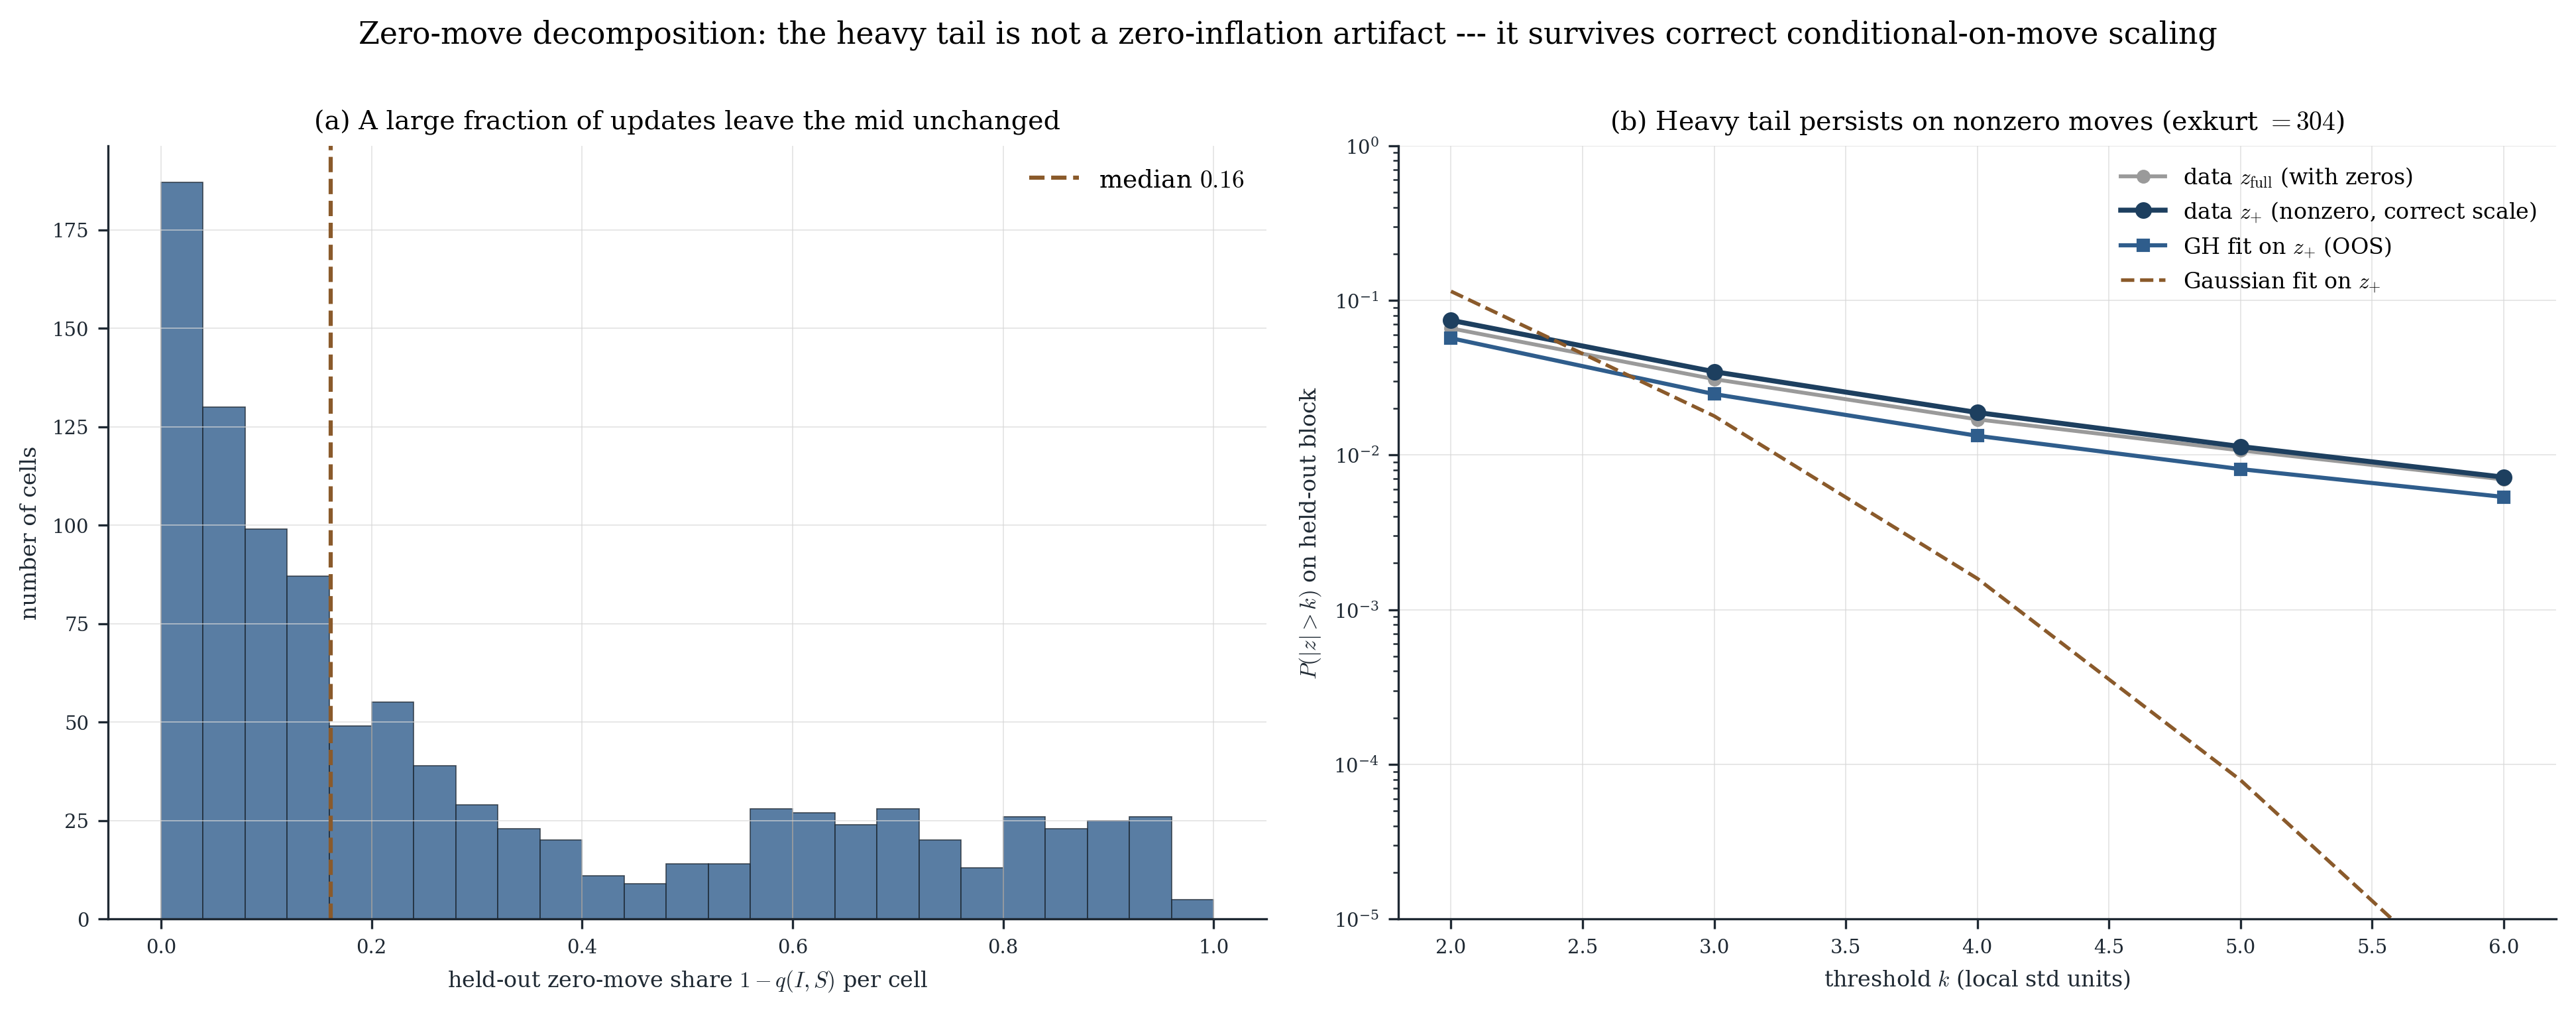
\includegraphics[width=\linewidth]{fig_zeromove.png}
\caption{The heavy tail is not a zero-inflation artifact. Panel~(a): the held-out zero-move
share $1-q(I,S)$ varies widely across state cells (median $0.16$, exceeding one half in many
cells). Panel~(b): tail exceedance $P(\lvert z\rvert>k)$ on held-out data for the full
residual (with zeros), the correctly-scaled nonzero residual $z_+$, and the Generalized
Hyperbolic and Gaussian laws fitted to $z_+$ out of sample. Removing the spike and correcting
the scaling lowers the tail, but it remains heavy and far above the Gaussian; the Generalized
Hyperbolic still tracks it.}
\label{fig:zeromove}
\end{figure}
\FloatBarrier

\subsection{Separate identification of scale and innovation shape (H4)}
\label{sub:res-ident}

Finally we test hypothesis~(H4): that the scale $\axx$ and the heavy-tailed
shape are distinct, individually necessary objects. We approach the factorisation
\eqref{eq:factorisation} from both sides.

\emph{The scale carries the state-dependence, and the multiplier does not.} The
realised held-out cell mean-square tracks the training $\axx$ across cells with a rank
correlation of $0.82$, while the realised multiplier
$\widehat G(c)=\E[(\Delta x)^2\given c]_{\mathrm{test}}/\axx^{\mathrm{train}}(c)$ has a
median of $1.22$ and, once de-biased against an independent scale estimate, shows no
material dependence on the state level (a log--log slope of $+0.12$). The
state-dependence of the move's size is carried by $\axx$; the multiplier is close to
state-neutral (Figure~\ref{fig:ident}).

\emph{Dividing out the shape recovers the scale.} Estimating the per-cell scale a
second way, by maximum likelihood under the fixed Generalized Hyperbolic shape, which
is far less sensitive to extreme observations than the second moment, recovers a
scale that agrees with $\sqrt{\axx}$ to within $1\%$ on the typical cell (median ratio
$0.991$, $95\%$ CI $[0.955,\,1.032]$), with a cross-cell rank correlation of $0.899$
($95\%$ CI $[0.881,\,0.914]$). A permutation placebo that randomly re-pairs the two
scale estimates collapses this association to $0.00\pm0.03$, placing the observed
value far into the tail of the null
($p<5\times10^{-4}$). The log--log slope of the two scales is $1.32$ ($95\%$ CI
$[1.26,\,1.38]$), slightly above one: the level agrees but the proportionality is not
exact, the same mild non-stationarity in tail thickness identified in
Section~\ref{sub:res-oos}.

\emph{The shape alone cannot stand in for the scale.} Conversely, removing only the
multiplier leaves $(\Delta x-b_x)/\sqrt{G}=\sqrt{\axx}\,Z$, which retains the
state-dependent variance and is therefore, pooled across states whose scales span
orders of magnitude, a scale mixture of normals, heavy-tailed and far from a single
Gaussian (Figure~\ref{fig:scale}, right). Only removing \emph{both} factors recovers a
standard normal. Scale and shape are thus separately identified and each is necessary:
$\axx$ supplies which states are violent, the heavy-tailed innovation supplies how
abruptly any given move can occur, and neither substitutes for the other. This is the
same multiplicative architecture as the Student-$t$ generalized autoregressive
conditional heteroskedasticity model, with the conditional variance indexed by the
contemporaneous book state rather than by the past of the return series.

\begin{figure}[!htbp]
\centering
\includegraphics[width=\linewidth]{sde_identifiability.png}
\caption{Scale versus multiplier. The realised held-out variance tracks the training
$\axx$ over orders of magnitude (left), while the realised multiplier is flat in the
state level (right): the state-dependence of the move's size is carried by $\axx$, not
by the innovation.}
\label{fig:ident}
\end{figure}

\begin{figure}[!htbp]
\centering
\includegraphics[width=\linewidth]{sde_scale_recovery.png}
\caption{Two views of the factorisation. Left: dividing out the Generalized
Hyperbolic shape recovers $\sqrt{\axx}$ (median ratio $0.99$). Right: dividing out
only the multiplier $\sqrt{G}$ leaves $\sqrt{\axx}\,Z$, which remains heavy-tailed, a
single universal kick cannot reproduce the state-dependent diffusion.}
\label{fig:scale}
\end{figure}
\FloatBarrier

\subsection{Benchmark comparisons with GARCH and HAR-RV}
\label{sub:res-garch}

This subsection is a benchmark, not the paper's contribution. The contribution, a
transferable, interpretable diffusion surface whose state-shape can be borrowed across
instruments after a one-scalar target volatility calibration
(Section~\ref{sub:res-axx}), is established above. The purpose here is narrower: to answer
the natural objection that a state-dependent conditional variance is merely a GARCH model
in disguise, and to locate the book-state diffusion relative to that standard benchmark.
The conclusion is that the two are complementary, not competing, and that the contribution is
the observable state surface and its tail-calibrated risk decomposition rather than dominance
over a fully estimated return-history benchmark.

The natural benchmark for a conditional-variance model is the generalized
autoregressive conditional heteroskedasticity family, which conditions the variance
on the past of the return series rather than on the contemporaneous book state. The
two information sets are different, and the relevant question is not which one wins a
one-step forecasting contest but what is gained by conditioning on the book state before the
move occurs. We test this directly. For
each instrument we fit a GARCH$(1,1)$ model on the training return series, on the
event clock, by Gaussian quasi-maximum likelihood, and filter its conditional
variance forward over the held-out returns. We then compare three variance
specifications by their out-of-sample mean Gaussian predictive log-likelihood, so
that the only difference between them is the variance forecast itself: the GARCH
forecast; the book-state diffusion $\axx(I,S)$; and a log-linear combination
$\log\sigma^2_n = c_0 + c_1\log\sigma^2_{\mathrm{GARCH},n} + c_2\log\axx(I_n,S_n)$
whose weights are estimated on the training set. Table~\ref{tab:garch} reports the
results across the $36$ instruments with sufficient data.

It is useful to make the notation explicit. The \emph{pure book-state SDE} developed
in Sections~\ref{sub:sde}--\ref{sub:innovation} is
\begin{equation}
  \Delta x_n
  =
  b_x(I_n,S_n)
  +
  \sqrt{\axx(I_n,S_n)}\,\eta_n,
  \qquad \eta_n \sim \GH,
  \label{eq:pure-book-sde}
\end{equation}
so its forecastable conditional variance is $\axx(I_n,S_n)$. The latent activity
multiplier inside the Generalized Hyperbolic innovation is not known before the move;
with the normalisation $\E[G_n\given I_n,S_n]=1$, it changes the \emph{shape} of the
shock distribution but not the ex-ante variance:
\[
  \Var(\Delta x_n\given I_n,S_n)=\axx(I_n,S_n).
\]
By contrast, the GARCH comparison also considers a \emph{hybrid predictive benchmark}
whose variance combines return-history information and book-state information,
\begin{equation}
  \log \sigma^2_{\mathrm{hyb},t}
  =
  c_0
  +
  c_1\log \sigma^2_{\mathrm{GARCH},n}
  +
  c_2\log \axx(I_n,S_n),
  \label{eq:hybrid-variance}
\end{equation}
and whose heavy-tailed version is
\begin{equation}
  \Delta x_n
  =
  b_x(I_n,S_n)
  +
  \sigma_{\mathrm{hyb},t}\,\eta_n,
  \qquad \eta_n \sim \GH.
  \label{eq:hybrid-gh}
\end{equation}
Thus ``combined variance + GH'' means GARCH plus $\axx(I,S)$ in the variance
forecast, with a Generalized Hyperbolic innovation. It is a forecasting benchmark,
not the pure structural model.

\begin{table}[!htbp]
\centering
\caption{Out-of-sample variance forecasting: book-state diffusion versus GARCH
(QSE, $36$ instruments, event clock). Entries are the mean Gaussian predictive
log-likelihood per held-out observation (higher is better), averaged across
instruments; the only difference between rows is the variance forecast. The
combination's weight on $\axx$ is positive for every instrument, while the combined
forecast improves on GARCH alone for $72\%$ of instruments.}
\label{tab:garch}
\small
\begin{tabular}{@{}lcc@{}}
\toprule
Variance specification & OOS log-likelihood / obs. & 95\% CI \\
\midrule
GARCH$(1,1)$ (return history)        & $-3.213$ & $[-3.394,\,-3.032]$ \\
Book-state diffusion $\axx(I,S)$     & $-3.601$ & $[-3.811,\,-3.391]$ \\
Combined (GARCH $\times$ book state) & $\mathbf{-3.192}$ & $[-3.379,\,-3.005]$ \\
\bottomrule
\end{tabular}
\begin{flushleft}
\footnotesize
Adding the book state to GARCH changes the mean log-likelihood by
$+0.021$ ($95\%$ CI $[+0.005,\,+0.037]$), positive for $72\%$ of names.
The fitted combination weight on $\axx$ is $c_2=+0.36$
($95\%$ CI $[+0.32,\,+0.40]$), positive for $100\%$ of names
(sign test $p\approx3\times10^{-11}$).
\end{flushleft}
\end{table}

\FloatBarrier

Three points follow, and we state them carefully. First, GARCH alone out-predicts the
book-state diffusion alone ($-3.20$ versus $-3.60$): the return history captures
volatility clustering, the fitted persistence $\alpha+\beta$ averages $0.993$, very
near a unit root, that a state-indexed surface, by construction, does not. We do not
claim that $\axx$ is a superior one-step variance forecaster, and consistent with the
modest forecasting skill reported in Section~\ref{sub:res-axx}, it is not. Second, and
this is the substantive result in the Gaussian variance comparison, the book state carries
information not spanned by the fitted GARCH recursion. The cleanest statement of this is
nonparametric: the estimated combination
places a \emph{positive} weight on $\axx$ for every one of the $36$ instruments
($c_2=+0.36$ on average). Under the null that the book state carries no incremental
information, the sign of that weight would be a coin flip, so a uniform run of $36$
positive signs is a sign test with $p\approx3\times10^{-11}$, decisive. The associated
gain in out-of-sample log-likelihood is positive but small, $+0.021$ on average and
positive for $26$ of the $36$ instruments (a far weaker sign test, $p\approx0.01$;
Figure~\ref{fig:garch}). We
therefore rest the claim on the uniform positivity of the weight, which is
overwhelming, rather than on the magnitude of the average gain, which is modest. Either
way, the contemporaneous book state carries conditional-variance information that the
return history does not contain, the two are complementary, not substitutes. Third,
beyond predictive accuracy there is a structural distinction that no forecasting
contest captures: a GARCH model is estimated separately for each series and its
parameters are not portable across instruments, whereas $\axx(I,S)$ is a single surface
whose state-shape transfers across QSE instruments (Section~\ref{sub:res-axx}); appendix
checks ask whether the same pattern is visible in smaller external samples
(Appendix~\ref{app:external}).

The conclusion strengthens, rather than weakens, on a regular wall-clock. Repeating the
comparison on fixed $60$-second bars, aggregating the book-state forecast to the
integrated conditional variance over each bar (the sum of the per-event $\axx$ within
the bar) and fitting the GARCH model on the regularly-spaced bar returns, the setting
for which it was designed, the book state becomes \emph{more} valuable. The combined
model now improves on GARCH out of sample by $+0.18$ in mean log-likelihood, positive
for $26$ of $30$ instruments (sign test $p\approx6\times10^{-5}$), with a positive
$\axx$ weight again for every instrument ($p\approx2\times10^{-9}$); and the book-state
forecast alone is now nearly the equal of GARCH ($-4.27$ versus $-4.23$). The reason is
instructive: at the event level the volatility clustering of consecutive updates is
extreme (persistence $0.99$), which makes the return history an unusually strong
forecaster and leaves little room for improvement, whereas at the one-minute level the
clustering is weaker (persistence $0.97$) and the contemporaneous book state contributes
substantially more. The complementarity is therefore robust to the choice of clock, and
the event-clock figures in Table~\ref{tab:garch} understate it.

The comparisons so far hold the innovation Gaussian, to isolate the variance
conditioning. We now relax that and let the heavy tail into the contest on both sides.
For each of the three variance forecasts we fit the residual distribution, a Gaussian,
a Student-$t$, and a symmetric Generalized Hyperbolic, each with location zero and a free
scale, on that model's own training residuals, and evaluate the out-of-sample predictive
log-likelihood. The Student-$t$ and Generalized Hyperbolic columns are therefore each
model's \emph{best-fit residual law}. This is not a fully joint re-estimation of a
GARCH-$t$ model; it is a deliberately parallel predictive-density comparison in which
the variance forecast is fixed first and the innovation law is then fitted to the
corresponding standardised residuals. Table~\ref{tab:grid} reports the full grid.

\begin{table}[!htbp]
\centering
\caption{Full predictive-density grid: out-of-sample mean log-likelihood per observation
(QSE, $36$ instruments, event clock) for each variance forecast (rows) under each
innovation law (columns). Each model's residual distribution is fitted on its own
training residuals; higher is better.}
\label{tab:grid}
\small
\begin{tabular}{@{}lccc@{}}
\toprule
Variance forecast & Gaussian & Student-$t$ & Gen.\ Hyperbolic \\
\midrule
GARCH$(1,1)$            & $-3.202$ & $-2.913$ & $-2.428$ \\
Book-state $\axx(I,S)$  & $-3.601$ & $-3.014$ & $-2.484$ \\
Combined               & $-3.192$ & $-2.907$ & $\mathbf{-2.427}$ \\
\bottomrule
\end{tabular}
\end{table}

The grid carries three messages, and they reinforce rather than complicate the paper's
position. First, \emph{the innovation shape dominates}: replacing the Gaussian by the
Generalized Hyperbolic raises the predictive log-likelihood by about $+0.8$ per
observation for \emph{every} variance specification, an order of magnitude larger than
any difference between variance specifications. The heavy tail, not the choice of variance
forecast, is the principal source of predictive gain, exactly as the centrality of the
tail result in Sections~\ref{sub:res-gh}--\ref{sub:res-oos} would lead one to expect.
Second, \emph{under a heavy tail the density-forecast increment disappears}: with a common Generalized Hyperbolic innovation the combined model improves on the GARCH
variance forecast out of sample by only $+0.001$ on average, positive for $19$ of $36$
instruments, a wash by the sign test ($p\approx0.87$). On the extended sample, then, once both
sides carry the heavy tail, the book-state variance is no longer a detectable improvement on the
return-history variance \emph{in average log-likelihood}; its value is the transferable,
interpretable state surface itself (Sections~\ref{sub:res-axx} and \ref{sub:res-ident}), not an
incremental one-step density gain. Third, \emph{the full model is competitive
with a Student-$t$ residual benchmark}: the combined variance with a Generalized
Hyperbolic innovation strongly out-predicts Gaussian GARCH (by $+0.78$) and has a higher
\emph{mean} log-likelihood than the GARCH variance with a fitted Student-$t$ residual
law ($+0.49$). The latter margin, however, is not significant across instruments ($23$
of $36$, $p\approx0.13$), and the Student-$t$ residual fit can be pulled toward very low degrees of
freedom by extreme observations (Section~\ref{sub:res-gh}). We therefore do not claim
to beat a fully estimated GARCH-$t$ model. The defensible claim is narrower and stronger:
once both sides are allowed heavy-tailed innovations, the state-dependent variance
remains a small but robust complement to the return-history variance, while the
Generalized Hyperbolic innovation is the larger quantitative improvement.

To make the last point precise rather than rest on the two-step residual fit, we estimate a
genuine \emph{jointly} maximum-likelihood GARCH-$t$ per instrument, the variance recursion
and the Student-$t$ degrees of freedom optimised together, the literature-standard benchmark.
The joint fit is well-behaved, with a median $\nu=3.6$ (a proper finite-variance law, unlike
the two-step free-$t$ that collapsed below two degrees of freedom), and scores $-2.562$ in
mean out-of-sample predictive log-likelihood. The full book-state model, combined variance
with a Generalized Hyperbolic innovation, scores $-2.427$: a higher mean by $+0.135$, but
positive for only $21$ of $36$ instruments (sign test $p\approx0.41$). The two are therefore
a statistical tie, which is exactly the honest reading. We do not beat a properly estimated
GARCH-$t$; we match it, while adding an interpretable, transferable state surface that
GARCH-$t$ does not provide.

The comparison is sharper against the standard realized-volatility benchmark. On fixed
$60$-second bars we fit the heterogeneous autoregressive realized-variance model
\citep[HAR-RV,][]{andersen2003} and compare it to the integrated book-state forecast (the sum
of the per-event $\axx$ within each bar). Here the book state is not merely complementary but
marginally superior on its own: with a Generalized Hyperbolic innovation, the book-state
forecast scores $-4.010$ against HAR-RV's $-4.047$, and their log-linear combination reaches
$-3.982$, improving on HAR-RV out of sample by $+0.065$ for $33$ of $36$ instruments (sign
test $p\approx2\times10^{-7}$). The contemporaneous order book thus carries
conditional-variance information that neither a return-history recursion nor a
realized-variance recursion contains.

The same conclusion is visible directly in the \emph{calibration} of the predictive
intervals (Figure~\ref{fig:garchcal}, Appendix~\ref{app:figures}).
Pooling all held-out moves, we ask how often each model's stated predictive interval
actually contains the realised move. A Gaussian GARCH \emph{under-states} tail risk, its
nominal $0.1\%$ two-sided tail is breached about eleven times too often, which is the
benchmark every other model must repair. The two Generalized Hyperbolic models and the
fitted Student-$t$ residual law all bring the extreme tail close to calibration: on the
extended sample the combined+GH benchmark sits at about $1.2$ times nominal at $0.1\%$ and
the Student-$t$ residual law is close to one across the whole range, while the pure
book-state model $a_{xx}(I,S)$+GH is closer than Gaussian GARCH but still over-exceeds at
$0.1\%$ (about three times nominal). The state-dependent heavy-tailed
model is therefore not merely competitive in average log-likelihood; it materially
improves tail calibration over the Gaussian benchmark, matching the Student-$t$ residual law
while adding a finite-variance, interpretable, transferable state surface.

Three caveats attend this comparison. The primary GARCH comparison is run on the event
clock, which is the native clock of the entire analysis but is not the regularly-spaced
clock for which the model was originally designed; the fixed-bar robustness check above
is precisely a check of this point, and the conclusion survives it. For computational
stability the GARCH
parameters are estimated on the most recent $12{,}000$ training observations of each
instrument, then filtered forward over the entire held-out sample. Finally, the primary
comparison in Table~\ref{tab:garch} uses a Gaussian predictive density on both sides, in
order to isolate the effect of the variance \emph{conditioning} from that of the
innovation \emph{shape}; the full predictive-density grid in Table~\ref{tab:grid} relaxes
this restriction in a residual-law comparison and confirms that the book-state increment
persists when heavy-tailed innovations are allowed on both sides.

% ===========================================================================
\section{Robustness and Limitations}
\label{sec:robustness}

Several features of the analysis warrant explicit qualification.

\emph{Statistical significance.} All structural claims are accompanied by bootstrap
confidence intervals and, where the relevant null is otherwise easy to beat, by
permutation placebos (Sections~\ref{sub:res-axx} and \ref{sub:res-ident}). We note
that the permutation placebo for the scale-recovery test is a deliberately weak bar:
because both scales are estimates from the same cell, any genuine pairing beats random
pairing, so the informative statistic there is the agreement in \emph{level} (median
ratio $0.99$), not the placebo.

\emph{Mild non-stationarity in tail thickness and regime robustness.} The out-of-sample
tail validation and the scale-recovery slope both detect a small, real drift in the
heaviness of the tail across the sample (the log--log slope of $1.32$, and the
consistent over/under-shoot across the two temporal directions). We treat the tail
thickness as constant in the baseline model; allowing it to vary slowly is a natural
refinement. We now report the cross-regime validation directly.

Splitting the 216 trading days by cross-instrument median $|\Delta x|$ gives 108 calm
and 108 stress days (cutoff $1.94$ bps). The diffusion surface transfers strongly across
regimes: the Spearman rank correlation of the cell-level $\axx$ estimates is $0.849$
when trained on calm days and scored on stress days, and $0.845$ in the reverse
direction, both above the adjacent-block baseline of $0.785$, which confirms that the
surface is not a calm-market artifact. The heavy-tailed innovation also remains valuable
out of regime: the Generalized Hyperbolic law beats the Gaussian by $+0.509$ and
$+0.452$ nats per observation in the two directions, compared with $+0.630$ in the
adjacent-block baseline. The modest reduction in tail gain across regimes is consistent
with the mild tail-thickness drift documented above: the pooled GH law, estimated once
on one regime type, partially tracks regime changes but does not fully account for the
slow drift.

\begin{figure}[!htbp]
\centering
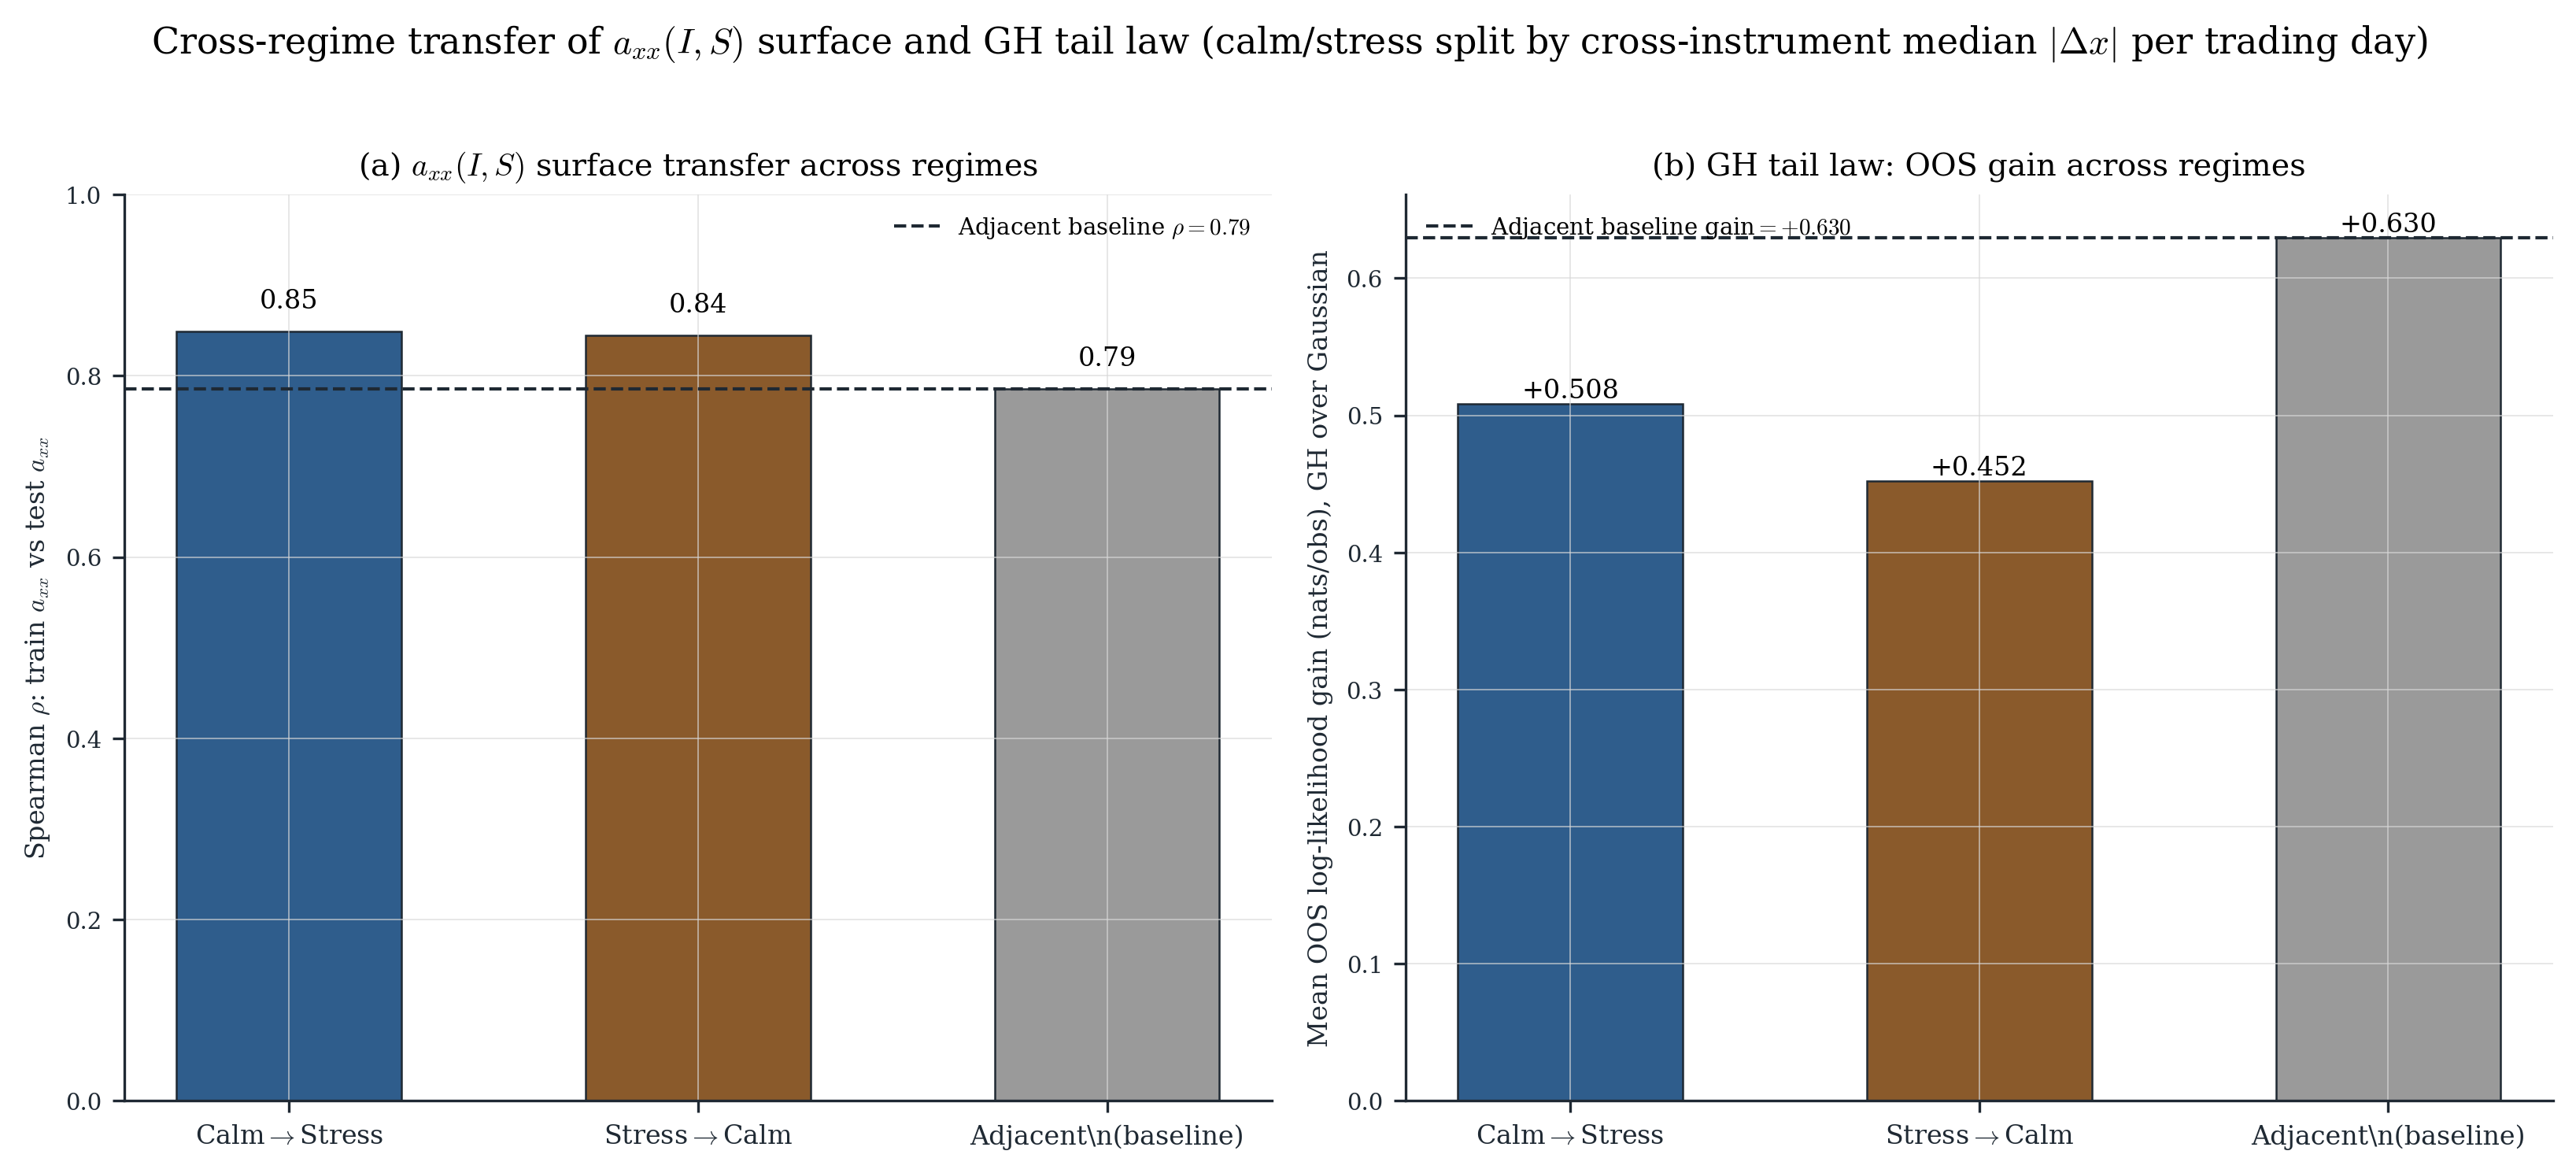
\includegraphics[width=\linewidth]{fig_regime_transfer.png}
\caption{Cross-regime transfer of the $\axx(I,S)$ surface and the Generalized Hyperbolic
tail law. Trading days are split into 108 calm and 108 stress days by cross-instrument
median $|\Delta x|$; surfaces and tail laws are estimated on one regime and scored on the
other. Panel~(a): Spearman rank correlation of trained vs held-out cell-level $\axx$
estimates; cross-regime correlations ($0.849$ and $0.845$) exceed the adjacent-block
baseline ($0.785$, dashed). Panel~(b): mean per-observation OOS log-likelihood gain of
the Generalized Hyperbolic over the Gaussian; all three experiments show clearly positive
gains, with a modest reduction cross-regime relative to the adjacent baseline,
consistent with mild tail non-stationarity.}
\label{fig:regimetransfer}
\end{figure}
\FloatBarrier

\emph{Sensitivity to extreme cells.} The large raw excess kurtosis of the pooled
residuals is driven by a small number of thinly populated cells; the maximum-likelihood
fits are correspondingly sensitive to those cells, which is why the maximum-likelihood
Student-$t$ is pulled to an infinite-variance regime. The Generalized Hyperbolic fit is
more stable, and the out-of-sample validation does not rely on the most extreme cells,
but the far-tail estimates should be read with this in mind. The five thinnest
instruments (AHCS, MHAR, QATI, MKDM, QIGD, each with fewer than 4,500 raw updates)
fall below the minimum observation threshold and are excluded from the pooled residuals
by the quality filter, so their joint exclusion is already in effect throughout the
analysis. As a further check, excluding the bottom quintile of the 36 instruments that
do pass the filter (7 instruments, 2.7\% of test observations) leaves the pooled
tail exceedances unchanged to two significant figures and raises the GH out-of-sample
gain by $+0.005$ nats per observation ($+0.516$ vs $+0.511$). The far-tail conclusions
are not driven by thin-name observations.

\emph{Symmetric innovation.} We use a symmetric Generalized Hyperbolic innovation.
Real returns may carry mild skewness, which an asymmetric member of the family would
capture; we leave this extension to future work.

\emph{Pooled, not per-state, mixing law.} We estimate a single innovation law for the
pooled residuals rather than a separate mixing law per state cell. The evidence in
Section~\ref{sub:res-ident} that the tail thickness is nearly state-neutral supports
this simplification, but a faint dependence remains and could be modelled.

\emph{Event-time clock and cross-venue comparability.} The model is written in event
time, so the microdiffusion is a variance per book update rather than per unit of
calendar time (Section~\ref{sub:continuous}). Magnitudes are therefore not directly
comparable across venues sampled on different clocks; the leading-order conversion
\eqref{eq:bridge} bridges the event and calendar clocks but ignores activity clustering,
and we accordingly keep the cross-venue claims qualitative (the \emph{shape} and
state-dependence recur), reserving quantitative comparisons for within-clock designs.

\emph{Is the pooled tail law instrument-specific?} Because the innovation is fitted to
residuals pooled across instruments of very different liquidity, one might worry that the
pooled tail conflates cross-instrument scale misfit with a genuine common shape. It does not.
Applying the same leave-one-instrument-out logic to the \emph{innovation law}, a Generalized
Hyperbolic fitted on the residuals of all \emph{other} instruments and scored on the held-out
one still beats the Gaussian out of sample for all but one of the $36$ instruments and retains $89\%$ of the gain
of the instrument's own fitted law (a mean loss of only $-0.051$ per observation). Splitting
the cross-section into liquidity terciles and fitting the law separately in each, the fitted
shape index moves by only $0.48$ and stays near the Normal-Inverse-Gaussian member in all
three (Figure~\ref{fig:ghloio}). The heavy-tailed shape is thus a common, instrument-neutral
feature, which is what justifies pooling it.

\begin{figure}[!htbp]
\centering
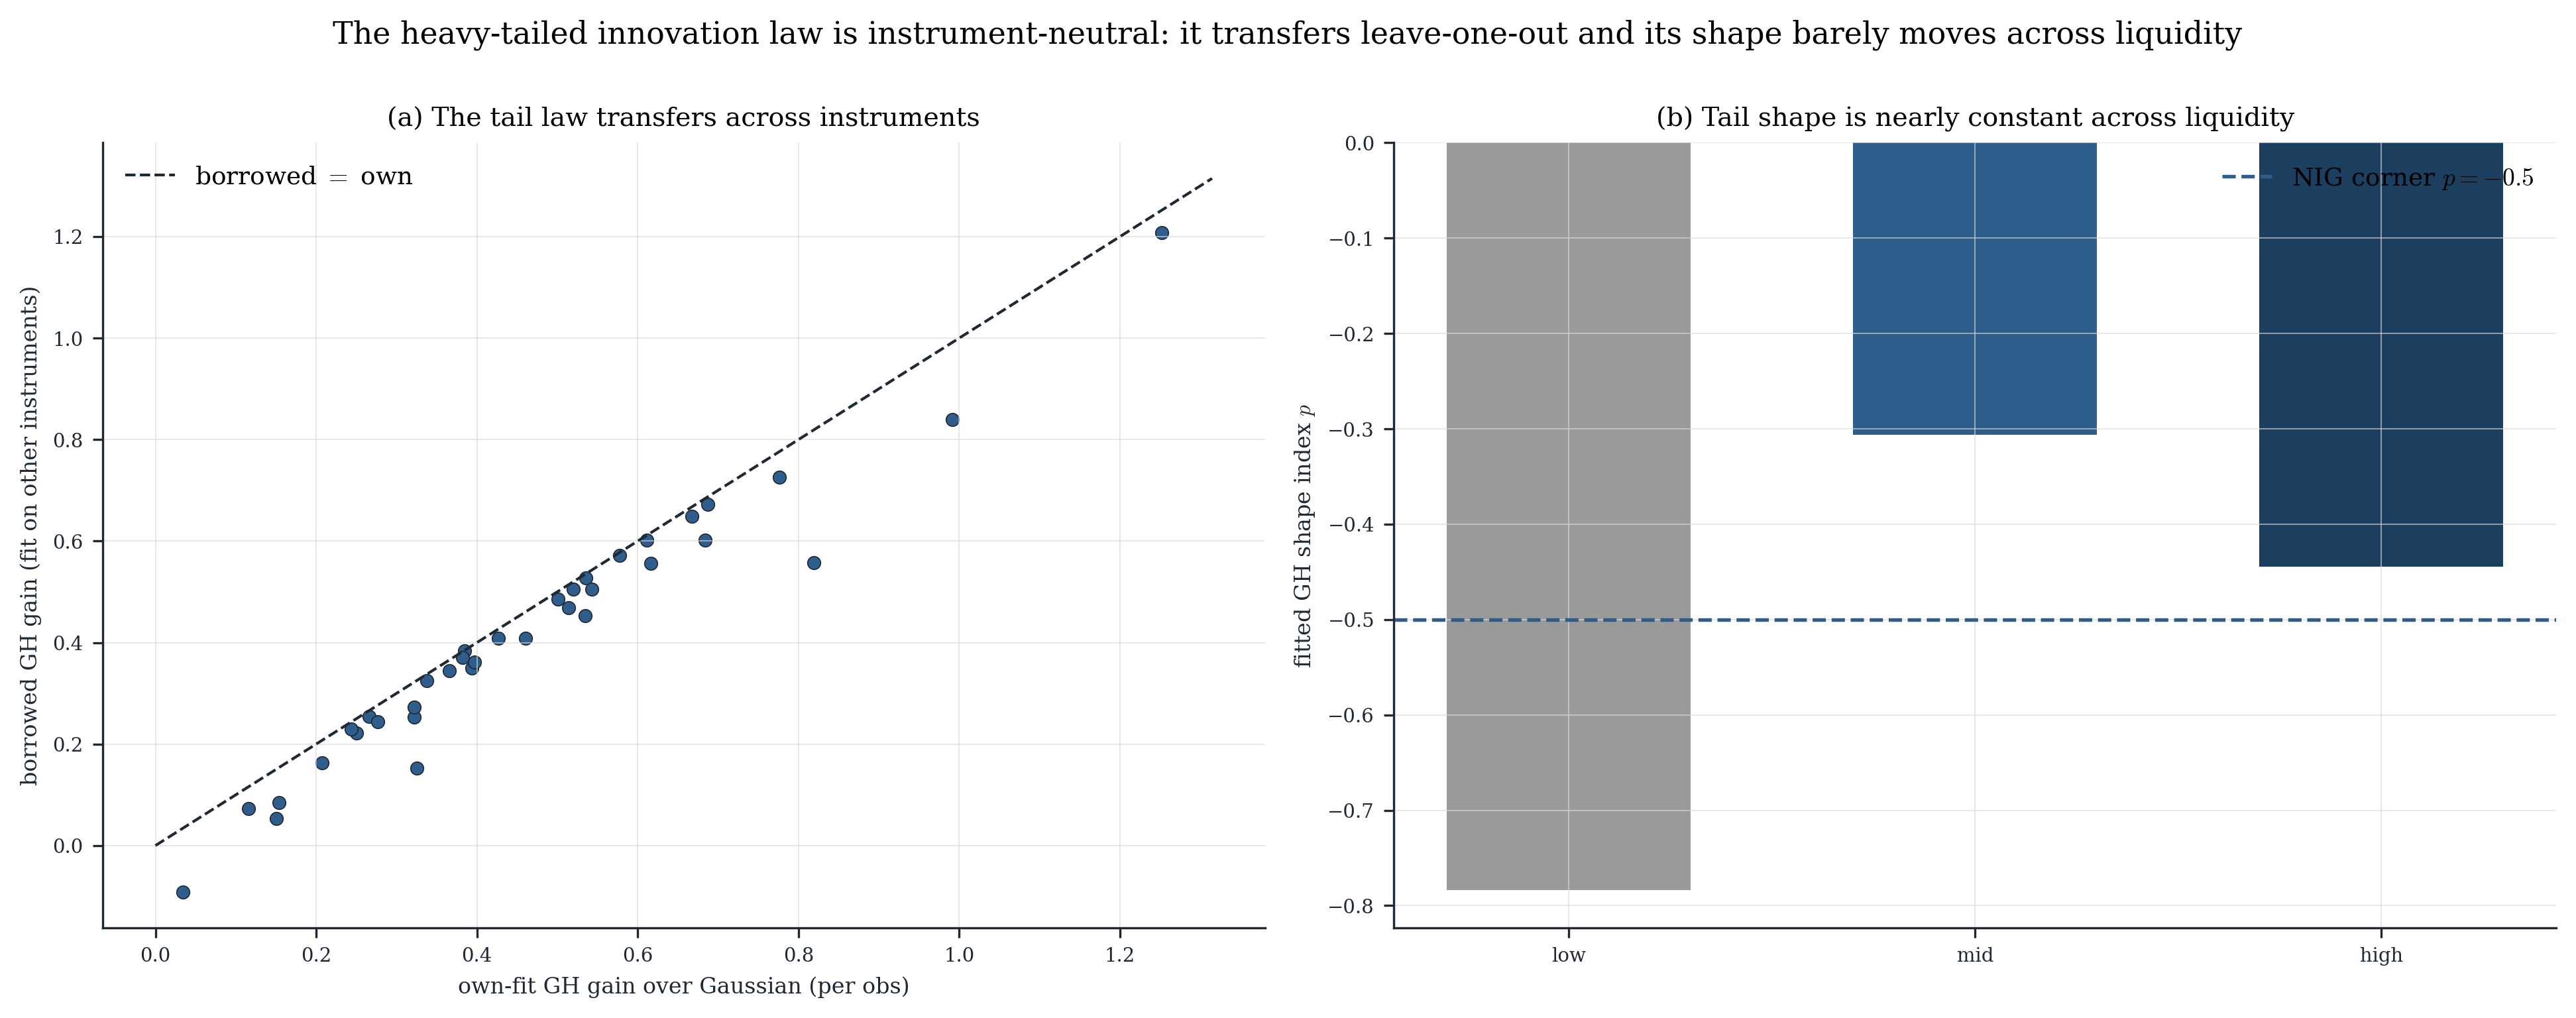
\includegraphics[width=\linewidth]{fig_gh_loio.png}
\caption{The innovation law is instrument-neutral. Panel~(a): for each instrument, the
out-of-sample log-likelihood gain over the Gaussian of a Generalized Hyperbolic law fitted on
\emph{other} instruments (borrowed) against the instrument's own fitted law; the borrowed law
keeps $89\%$ of the own-fit gain and is positive for all but one name. Panel~(b): the fitted shape
index $p$ by liquidity tercile varies by only $0.48$ and sits near the Normal-Inverse-Gaussian
corner throughout. Pooling the tail law across instruments is therefore justified.}
\label{fig:ghloio}
\end{figure}
\FloatBarrier

% ===========================================================================
\section{Discussion}
\label{sec:discussion}

The object this paper introduces, a conditional price diffusion that is a function of
the contemporaneous order-book state, transfers out of sample, and pairs with the
microprice drift in a single stochastic equation, extends the microprice programme
to its second-moment side. Three points frame its scope and use.

First, the model is microstructure-native in a way that distinguishes it from the
conditional-volatility tradition. The conditional variance is read from the book at
the moment of the move, not inferred from the recent past of the return series, and it
is a surface over book states rather than a recursion in time. That is what allows the
surface to be transferred across days and across instruments, and it is the empirical
content of the paper's structural claim.

Second, the equation is immediately usable. Because the drift and the diffusion are
estimated functions of an observable state, the equation can be simulated forward on
any realised sequence of imbalance and spread to produce conditional distributions of
future price moves, including their tails; and because the innovation is a calibrated,
out-of-sample-validated heavy-tailed law, those simulated tails are realistic rather
than Gaussian. This is a state-conditional risk object of direct practical interest.

To make this concrete, the equation delivers at every step a one-step-ahead predictive
interval for the price, centred at $x_n+b_x(I_n,S_n)$ and bracketed by
$\sqrt{\axx(I_n,S_n)}\,q^{\GH}_{\alpha}$, the quantiles of the heavy-tailed innovation.
Figure~\ref{fig:band} draws this band along a held-out session and separates its width
into the two sources the model identifies: an inner layer set by the state-dependent
scale $\axx(I,S)$, which makes the band \emph{breathe}, narrow in calm configurations,
wide when the spread opens or the book tilts, and an outer layer contributed by the
Generalized Hyperbolic tail, which extends the band at high confidence and absorbs the
abrupt moves that a Gaussian interval of the same scale would miss. Two cautions should
be read with the figure. It is a genuine \emph{ex-ante} interval, each band uses only
information available before the move, and its aggregate validity is precisely what the
calibration analysis of Section~\ref{sub:res-garch} establishes; the figure illustrates a
single session and is not itself independent evidence. And it is a forecast of
\emph{risk}, not of \emph{direction}: because the drift is small the band is centred close
to the current price, so the model's content is the width, shape, and tail of the
next-price distribution rather than a directional point prediction.

\begin{figure}[!htbp]
\centering
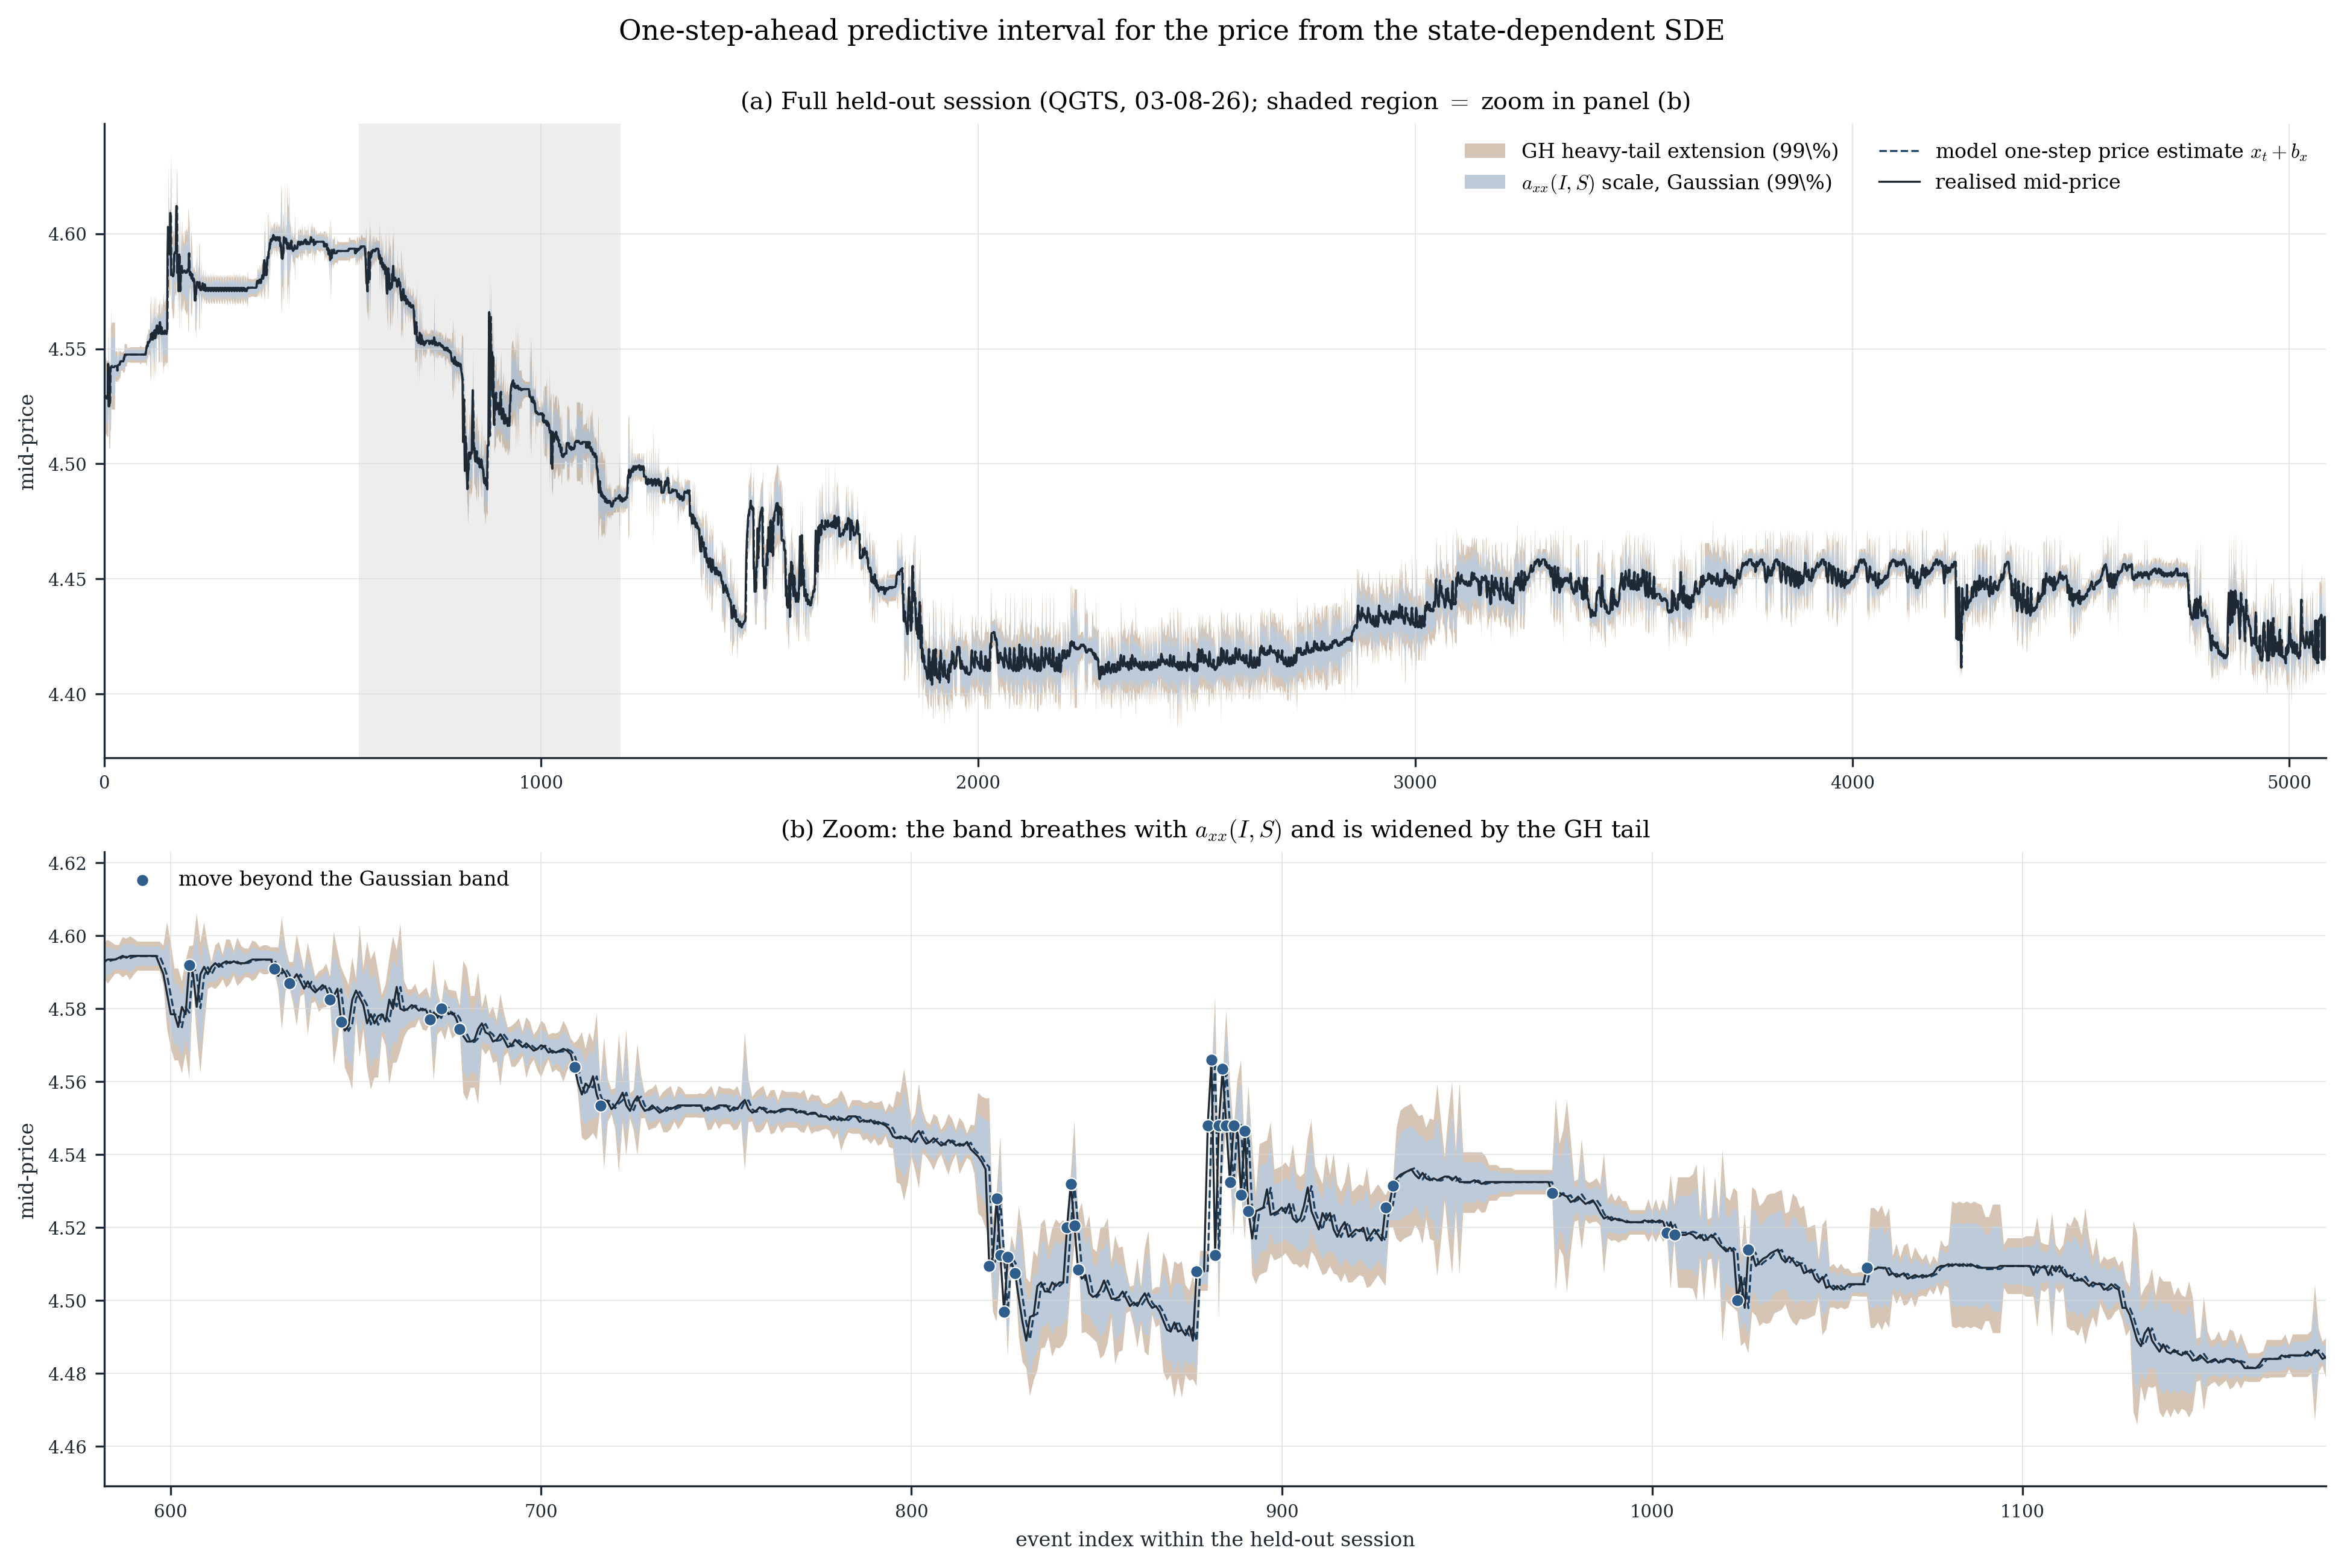
\includegraphics[width=\linewidth]{fig_price_band.png}
\caption{The state-dependent SDE as a predictive interval for the price, illustrated on one
held-out session. Panel~(a) shows the full session, the realised mid-price with the
predictive band, and the shaded region marks the window magnified in panel~(b). At each
step the band is the one-step-ahead $99\%$ predictive interval for the price, centred at
$x_n+b_x(I_n,S_n)$, with its width split into two layers: an inner layer set by the
state-dependent scale $\axx(I,S)$ (with a Gaussian shape), which breathes with the book
state, narrow in calm stretches, wide around the volatile region, and an outer layer
contributed by the Generalized Hyperbolic heavy tail, which extends the interval at high
confidence. Marked points in panel~(b) are realised moves that pierce the Gaussian band
and therefore illustrate where the Gaussian interval is too narrow. The interval is
ex-ante and forecasts risk, not direction (the centre tracks the current price because
the drift is small); its calibration is validated in aggregate in
Section~\ref{sub:res-garch}.}
\label{fig:band}
\end{figure}

The same held-out instrument can also be viewed distributionally
(Appendix Figure~\ref{fig:modelreal}). That supplementary figure separates the two
ingredients of the band: the standardised one-step returns are much closer to the fitted
Generalized Hyperbolic law than to a Gaussian, and the distribution of the model's
conditional variance $\axx(I,S)$ along the realised held-out state path is close to the
held-out per-state variance distribution over its bulk. The remaining discrepancy is in
the far right tail, where the realised variance distribution is heavier. This is the
same boundary identified earlier: a static per-state surface captures the state-driven
variance level, but it does not reproduce all transient high-variance bursts generated by
volatility clustering (Sections~\ref{sub:res-axx} and \ref{sub:res-garch}). We keep that
single-instrument comparison in the appendix because the pooled evidence in
Sections~\ref{sub:res-axx} and \ref{sub:res-gh} is the inferential result.

Third, the predictive interval has economic content that can be scored formally.

\subsection{Intraday VaR backtest}
\label{sub:var-backtest}

The predictive interval in Figure~\ref{fig:band} is a single-session illustration.
Its aggregate validity can be evaluated as a formal intraday VaR backtest. At each
step $n$ in the held-out sessions, the model delivers a two-sided interval
\begin{equation}
\text{VaR}_{\alpha,n}
= \bigl[\,b_x(I_n,S_n) \pm \sqrt{\axx(I_n,S_n)}\,q^{\GH}_{1-\alpha/2}\,\bigr],
\label{eq:var}
\end{equation}
where $q^{\GH}_{1-\alpha/2}$ is the upper $(1-\alpha/2)$ quantile of the fitted
unit-variance Generalized Hyperbolic innovation. A violation occurs when
$|\Delta x_n - b_x(I_n,S_n)| > \sqrt{\axx(I_n,S_n)}\,q^{\GH}_{1-\alpha/2}$.
We apply the Kupiec~\citep{kupiec1995} unconditional coverage test ($\mathrm{LR}_{\mathrm{uc}}$,
$\chi^2(1)$) and the Christoffersen~\citep{christoffersen1998} independence test
($\mathrm{LR}_{\mathrm{ind}}$, $\chi^2(1)$) to the resulting violation sequences on all
36 QSE instruments, for $\alpha \in \{0.01, 0.05\}$. Transition counts for the
independence test are accumulated within sessions only; no transition is recorded across
session boundaries.

The backtest confirms the economic value of the heavy-tailed innovation while also
exposing the model's remaining limitation. At $\alpha = 0.01$, the GH model produces a
median violation rate of $\hat{\pi} = 0.0133$ across instruments, against $0.0275$ for
the Gaussian VaR of the same width. The heavy-tailed innovation roughly halves the
far-tail under-coverage relative to the Gaussian benchmark. However, the Kupiec test
rejects formal unconditional coverage for 33 of 36 instruments under GH (3 of 36 pass),
compared with 35 of 36 rejections under Gaussian. At $\alpha = 0.05$, GH and Gaussian
are closer: median violation rates are $0.0588$ and $0.0494$ respectively, with 4 and 3
instruments passing $\mathrm{LR}_{\mathrm{uc}}$. The result is not full VaR calibration;
it is a material reduction in Gaussian tail under-coverage, consistent with the mild
tail non-stationarity documented in Section~\ref{sec:robustness}: the single pooled GH
law, estimated once on the training split, captures the cross-sectional shape of the
tail but cannot fully track the slow drift in tail thickness across regimes.

\begin{figure}[!htbp]
\centering
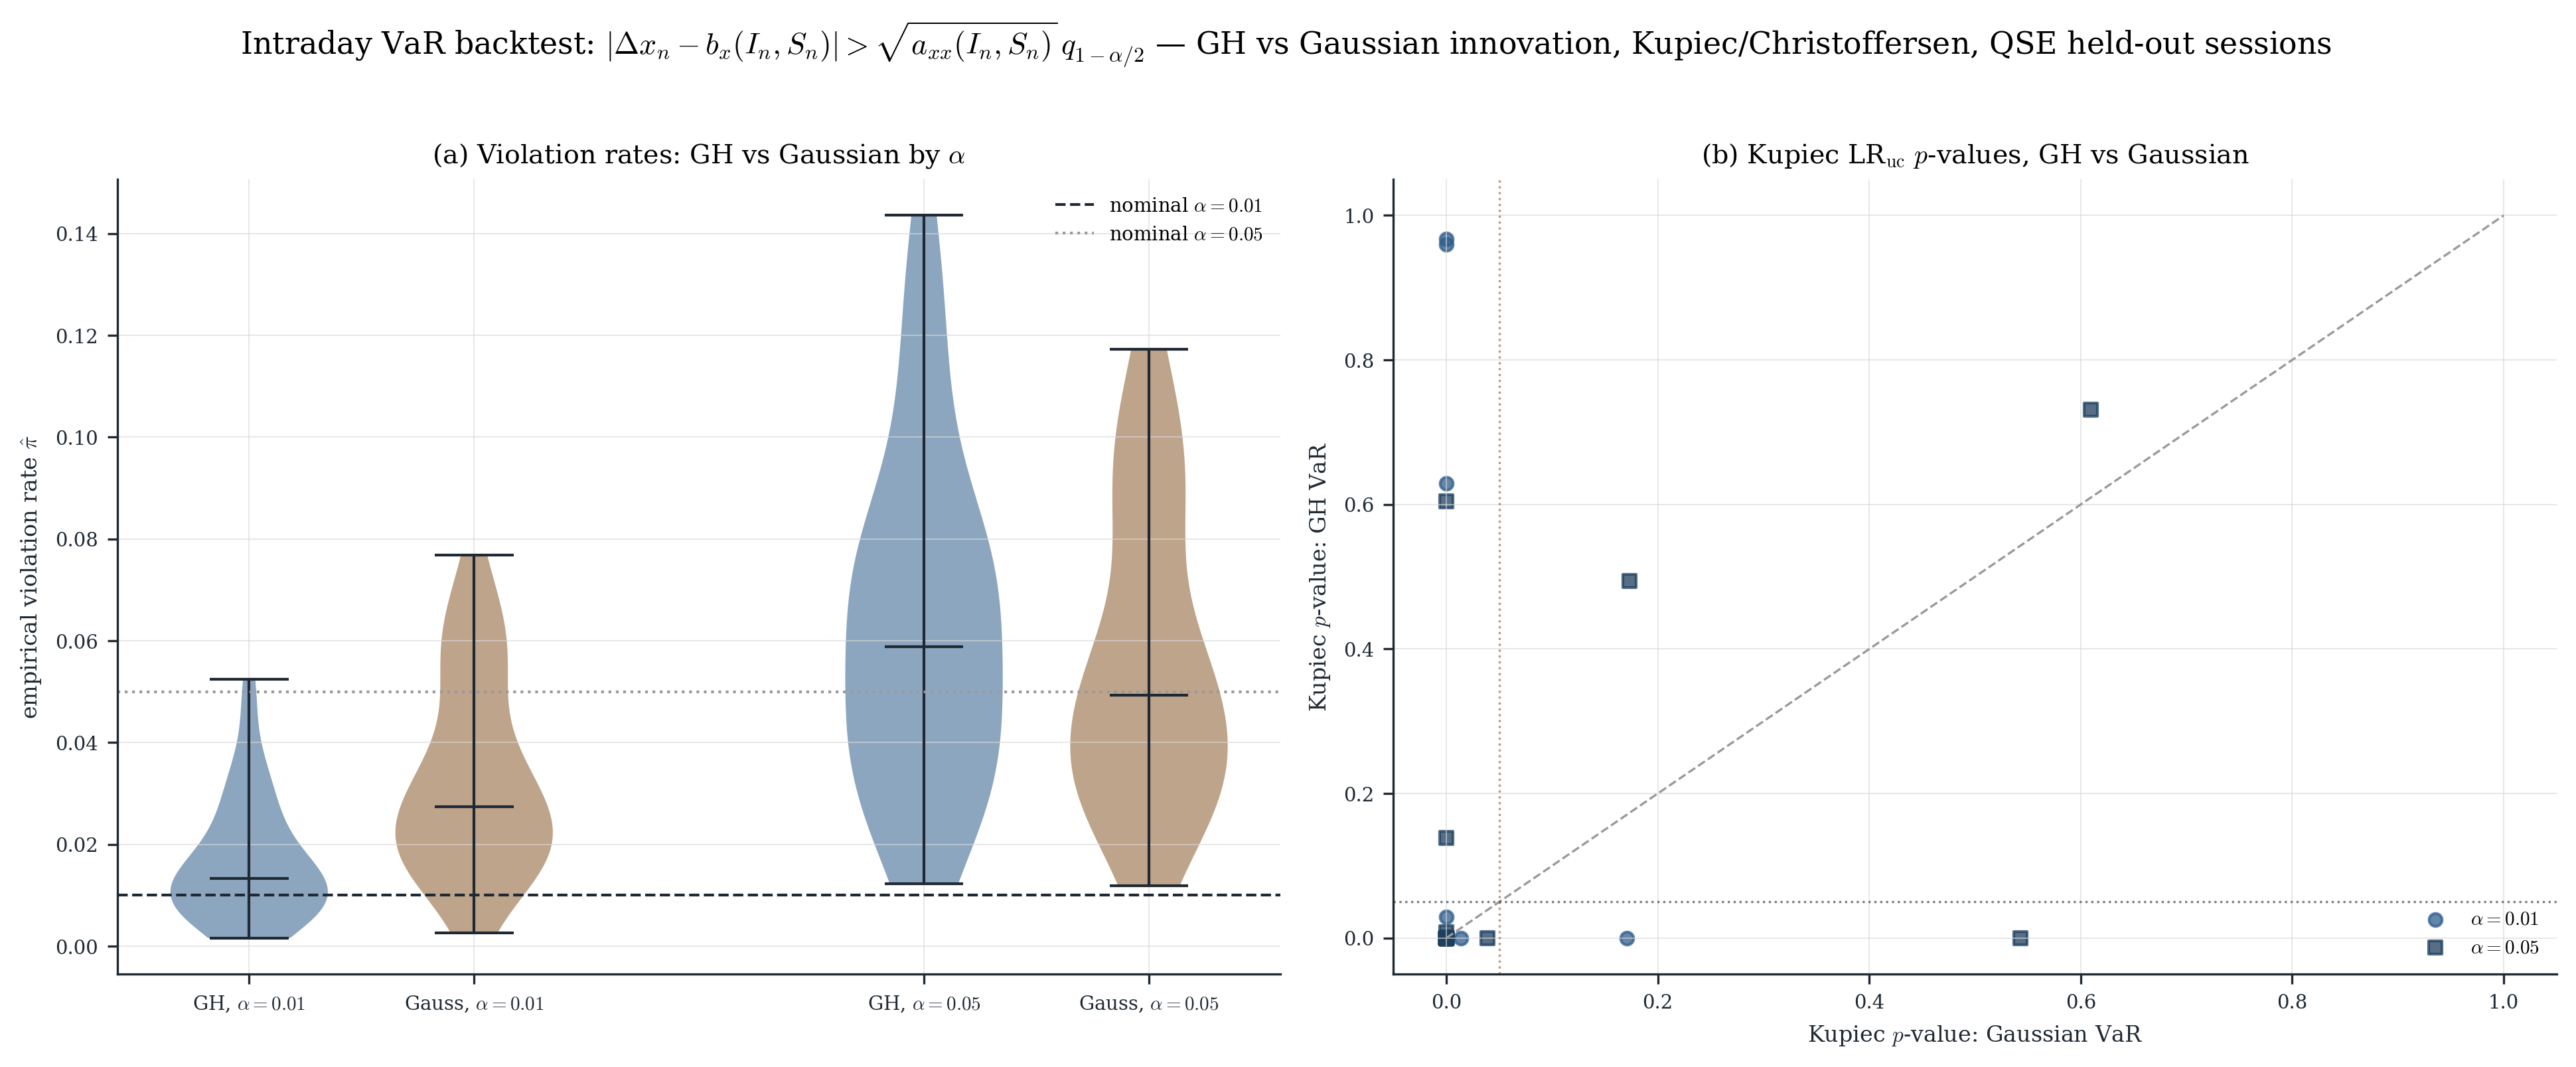
\includegraphics[width=\linewidth]{fig_var_backtest.png}
\caption{Intraday VaR backtest on held-out QSE sessions, $\alpha \in \{0.01,0.05\}$.
Panel~(a): violin plots of empirical violation rates $\hat{\pi}$ across instruments for
the GH and Gaussian VaR; horizontal dashed lines mark the nominal levels.
Panel~(b): Kupiec $\mathrm{LR}_{\mathrm{uc}}$ $p$-values for GH versus Gaussian;
points above the diagonal indicate instruments where the GH model is better
calibrated. The GH model halves the median far-tail violation rate relative to the
Gaussian benchmark ($0.0133$ vs.\ $0.0275$ at $\alpha{=}0.01$) but does not achieve
formal unconditional coverage on most instruments, consistent with the mild tail
non-stationarity noted in Section~\ref{sec:robustness}.}
\label{fig:varbacktest}
\end{figure}
\FloatBarrier

Fourth, the framework rests on a single closure (Assumption~\ref{ass:closure}): that
the unresolved part of the book enters the next increment only through the statistics
of the fluctuation, summarised by the conditional diffusion. We have treated that
closure purely as an econometric device and have validated its testable consequence,
the transfer of $\axx$. Whether the same validated diffusion supports a more structural,
fluctuation-based reading, and any market-stability diagnostics that might follow from
it, is a separate question that we do not pursue here.

% ===========================================================================
\FloatBarrier
\section{Conclusion}
\label{sec:conclusion}

The microprice models the conditional drift of price given the state of the limit
order book; its missing complement is the microdiffusion. This paper has
defined the microdiffusion as a surface $\axx(I,S)$ over the imbalance and the spread,
shown on the primary QSE sample that it is a genuine structural object that transfers
out of sample (split-half reliability $0.95$, cross-day transfer $0.48$, against a
null of zero), and assembled it with the
Stoikov drift into a state-dependent event-time stochastic equation. We have shown
that this equation has the right scale but, under a Gaussian innovation, the wrong
tails, and that a symmetric, unit-variance Generalized Hyperbolic innovation, a
normal variance mixture with a Generalized-Inverse-Gaussian mixing variable, repairs
the tails and validates out of sample, with a positive out-of-sample log-likelihood
gain over the Gaussian and a tail predicted to within a small factor where the
Gaussian errs by orders of magnitude. Finally, we have shown that the scale and the
shape are separately identified and individually necessary. Along the way the analysis
isolates a \emph{second-moment} role for order-book imbalance, distinct from its
first-moment role in the microprice: holding the tick mechanics fixed, the magnitude of
the imbalance, on either side, inflates the conditional variance, even though the level
of the surface across states is carried mainly by the spread, and the within-spread
imbalance shape does not reliably transfer day to day.

The result is a microstructure-native, state-indexed, transferable, heavy-tailed model of
conditional price diffusion that is both rigorous and immediately usable. It turns the
microprice framework from a conditional-drift model into a full conditional-distribution
model for short-horizon price risk: read from the visible book rather than from the history
of returns, it assigns two book states with the same mid-price, a deep, balanced, tight book
and a fragile, one-sided, wide one, visibly different next-move risk, which is precisely the
distinction a return-history volatility model cannot draw in real time. It is on this validated
object that further, more interpretive analysis can rest.

% ===========================================================================
\FloatBarrier
\clearpage
\bibliographystyle{plainnat}
\bibliography{references}

% ===========================================================================
\FloatBarrier
\clearpage
\appendix

\section{Supplementary derivations}
\label{app:derivations}
This appendix gives the steps stated as results in the main text, in event time.

\subsection{Event-time mean-square decomposition}
\label{app:msq}
For any state $(I,S)$, applying $\E[Y^2]=\Var(Y)+(\E Y)^2$ to $Y=\Delta x_n$ conditional on
$(I_n,S_n)=(I,S)$ gives, with the definitions \eqref{eq:drift}--\eqref{eq:axx-def}, the
exact identity \eqref{eq:msq},
\begin{equation*}
  \E\!\left[(\Delta x_n)^2 \mid I,S\right] = \axx(I,S) + b_x(I,S)^2 .
\end{equation*}
This is exact in event time; it is not an expansion in a small step $\Delta t$. The
squared-drift term is negligible for an \emph{empirical} reason rather than an asymptotic
one: at the one-update horizon the fitted $b_x$ is of order $10^{-7}$ in log units while
$\sqrt{\axx}$ is of order $10^{-4}$, so $b_x^2/\axx \sim 10^{-6}$, and the uncentred mean
square \eqref{eq:axx-surface} coincides with the centred microdiffusion to six significant
figures. The centred form is used only in the identification of
Section~\ref{sub:identification}.

\subsection{Variance-mixture moments and the kurtosis identity}
\label{app:moments}
For $\eta_n=\sqrt{G_n}\,N_n$ with $N_n\sim\Norm(0,1)\perp G_n$, independence and the
symmetry of $N_n$ ($\E N_n=0$, $\E N_n^2=1$, $\E N_n^4=3$) give
\eqref{eq:mix-mean}--\eqref{eq:mix-fourth}, namely $\E[\eta_n]=0$, $\E[\eta_n^2]=\E[G_n]$,
and $\E[\eta_n^4]=3\,\E[G_n^2]$. Under the normalisation $\E[G_n]=1$ the excess kurtosis is
\begin{equation*}
  \kappa(\eta_n) = \frac{3\,\E[G_n^2]}{(\E[G_n])^2} - 3 = 3\bigl(\E[G_n^2]-1\bigr) = 3\,\Var(G_n),
\end{equation*}
the identity \eqref{eq:kurtosis-identity}: once the mixing variable is normalised to unit
mean, a single number, the variance of $G_n$, governs the tail heaviness.

\subsection{From GIG to GH and the unit-mean rescaling}
\label{app:giggh}
When $G_n\sim\GIG(\lambda,\chi,\psi)$, the mixture $\eta_n=\sqrt{G_n}\,N_n$ is a symmetric
Generalized Hyperbolic law \eqref{eq:gig-gh}. The normalisation $\E[G_n]=1$ is not
automatic: for a generic GIG variable
\begin{equation*}
  \E[G_n] = \sqrt{\tfrac{\chi}{\psi}}\;
  \frac{K_{\lambda+1}\!\left(\sqrt{\chi\psi}\right)}{K_{\lambda}\!\left(\sqrt{\chi\psi}\right)},
\end{equation*}
with $K_\nu$ the modified Bessel function of the second kind. We rescale the fitted mixing
law so that this equals one, which keeps the entire scale of the move in
$\sqrt{\axx(I,S)}$ and leaves $G_n$ to carry only the residual tail risk. The fits
concentrate near the Normal-Inverse-Gaussian member, $\lambda=-\tfrac12$.

\subsection{Identification of scale and shape}
\label{app:ident}
From the factorisation \eqref{eq:factorisation}, $(\Delta x_n-b_x)^2/\axx(I,S)=G_n N_n^2$
with $\E[G_n N_n^2\mid I,S]=\E[G_n\mid I,S]\,\E[N_n^2]=1$, so a single observation reveals
only the product $G_n N_n^2$, never $G_n$ alone. Identification is therefore at the level
of conditional means: the two conditions $\axx\in\sigma(I,S)$ and $\E[G_n\mid I,S]=1$
render the decomposition $V_n=\axx(I,S)\,G_n$ unique and give
$\axx(I,S)=\E[(\Delta x_n-b_x)^2\mid I,S]$, equations
\eqref{eq:axx-identified}--\eqref{eq:gz2}.

\subsection{Cross-clock rate bridge}
\label{app:bridge}
The microdiffusion \eqref{eq:axx-surface} is a variance per book update. To compare venues
sampled on different clocks, write $\Delta\tau_n$ for the elapsed clock time between updates
$n$ and $n+1$. Over a fixed calendar interval $[0,T]$ in a state with conditional mean
inter-arrival $\E[\Delta\tau_n\mid I,S]$, the number of updates is
$T/\E[\Delta\tau_n\mid I,S]$ to leading order, and, under near-uncorrelated increments,
consistent with the near-martingale property, the calendar-time variance accumulates
additively across updates. Equating the per-update and per-calendar-time variance
accumulation gives
\begin{equation}
  a^{\mathrm{cal}}_{xx}(I,S)
  \;\approx\;
  \frac{a^{\mathrm{event}}_{xx}(I,S)}{\E\!\left[\Delta\tau_n \mid I_n=I,\,S_n=S\right]} .
  \label{eq:bridge}
\end{equation}
This is a leading-order bridge: it ignores activity clustering, under which the
per-interval update count is itself bursty and contributes higher-order corrections. It is
used only for the external-sample comparability of Appendix~\ref{app:external} and does not
enter the primary QSE event-time results.

\subsection{Continuous-time interpretation}
\label{app:continuous}
The Gaussian benchmark \eqref{eq:sde-cont} is a local It\^o-diffusion conditional on the
observed book state and is not a closed continuous-time model unless the joint dynamics of
$(I_t,S_t)$ are specified. The heavy-tailed case \eqref{eq:gh-sde} requires promoting the
mixing variable to a positive adapted process $G_t$ with the augmented state $Y_t=(F_t,G_t)$,
a subordination or Barndorff-Nielsen--Shephard construction \citep{barndorffnielsen1997};
estimating that latent process is outside this paper's event-time scope
(Section~\ref{sub:continuous}).

\section{Estimation and protocol details}
\label{app:estimation}
This appendix records the concrete estimation choices and procedures abbreviated in
Sections~\ref{sec:data}--\ref{sec:results}, to the level needed for replication.

\subsection{State construction and binning}
\label{app:binning}
The conditioning state is $(I,S)$. The imbalance axis is partitioned into
$N_I=10$ equal-width bins on $[-1,1]$; the relative spread is partitioned into
$M_S=3$ terciles whose cut-points are estimated on the training partition of each
instrument and then applied unchanged to its test partition. This yields up to
$N_I\times M_S=30$ state cells per instrument. A cell is retained only if it carries at
least $50$ held-out observations, which trims the sparsest corners of the grid
(Appendix~\ref{app:figures}); all reported transfer and tail statistics are computed on
retained cells. Sessions are split chronologically $60/40$ into training and test, and a
symbol-session enters the panel only if it clears $1{,}500$ cleaned events.

\subsection{Out-of-sample protocols}
\label{app:protocols-detail}
The four protocols of Section~\ref{sub:protocols} are: (i) \emph{cross-day transfer}, 
train $\axx$ on the training days, correlate (Spearman) with the realised held-out cell
mean-square, against a label-shuffled placebo; (ii) \emph{split-half reliability}, two
disjoint training blocks, correlate the two $\axx$ estimates; (iii) \emph{fresh-split tail
validation}, fit the innovation on one held-out temporal block and score it on the
disjoint other, in both directions; (iv) \emph{uncertainty}, bootstrap resampling the
unit of analysis (instrument or cell) and, where a sharper null helps, permutation tests.
Nothing estimated on training data is re-estimated on the test data.

\subsection{Innovation fitting}
\label{app:ghfit}
The symmetric, centred, unit-scale Generalized Hyperbolic innovation is fitted by maximum
likelihood to the pooled standardised residuals; the optimisation uses a deterministic
subsample for speed and is insensitive to the subsample size at the panel scale. We also
fit two Student-$t$ comparators, one by maximum likelihood, one by kurtosis
matching, and report tail-exceedance probabilities at a far-tail cap (the $99.9\%$
quantile) so that a handful of extreme observations do not dominate. The fitted GH shape
concentrates at the Normal-Inverse-Gaussian corner ($\lambda=-\tfrac12$).

\subsection{Benchmark specifications}
\label{app:benchmarks}
The GARCH$(1,1)$ benchmark is estimated by Gaussian quasi-maximum likelihood on the most
recent $12{,}000$ training observations of each instrument and filtered forward over the
held-out sample. The joint GARCH-$t$ benchmark estimates the variance recursion and the
Student-$t$ degrees of freedom together by maximum likelihood. The HAR-RV benchmark is fit
on fixed $60$-second realised-variance bars. The combined forecast is the log-linear
blend $\log\sigma^2_n = c_0 + c_1\log\sigma^2_{\mathrm{GARCH},n} + c_2\log\axx(I_n,S_n)$,
with weights estimated on the training set. All comparisons are on the native event clock
unless a fixed-bar robustness check is stated.

\subsection{Tick recovery and spread-in-ticks stratification}
\label{app:tick}
The exact tick size is recovered per instrument from the decimal grid of quoted prices.
The tick-control test stratifies by spread measured in ticks ($1$, $2$, $3$, $\ge 4$) so
that the mechanical spread--move relationship is held fixed by construction, and measures
the imbalance shape within each stratum after log-demeaning $\axx$ within each
instrument$\times$stratum (Section~\ref{sub:res-axx}).

\subsection{Zero-move two-part decomposition}
\label{app:zeromove-detail}
Writing $q(I,S)=\mathbb{P}(\Delta x_n\neq 0\mid I,S)$ and
$a_+(I,S)=\E[(\Delta x_n-b_x)^2\mid \Delta x_n\neq 0, I,S]$, the microdiffusion factors as
$\axx = q\,a_+ + (1-q)b_x^2 \approx q\,a_+$. Nonzero moves are standardised by the
conditional-on-move scale $z_+=(\Delta x_n-b_x)/\sqrt{a_+}$, which has unit variance on the
moves, rather than by $\sqrt{\axx}$, which would inflate their variance by $1/q$
(Section~\ref{sub:res-zeromove}).

\section{External-sample robustness}
\label{app:external}
This appendix reports the limited external checks used to assess whether the QSE
results are obviously venue-specific. These checks are deliberately separated from
the main empirical results because neither external sample matches the strength of
the QSE design: the cryptocurrency data contain only three assets on a one-second
clock, and the LOBSTER sample contains only one trading day.

\subsection{Cryptocurrency and LOBSTER transfer}
\label{app:ext-transfer}
On the cryptocurrency sample, the diffusion surface transfers across calendar-day
blocks with a joint $(I,S)$ rank correlation of $0.757$ ($95\%$
instrument-clustered interval $[0.622,\,0.861]$), while the shuffled-cell placebo is
close to zero. This supports the main structural claim, but it should be read as a
robustness replication rather than as a second full venue study because the sample
contains only BTC, ETH, and ADA, and the ``sessions'' are arbitrary UTC-day
partitions of a continuous 24/7 market. On the single-day U.S.\ equity LOBSTER
sample, the diffusion surface is estimable and exhibits the same qualitative
dependence on the book state, but the absence of multiple days prevents the
cross-day transfer and heavy-tailed out-of-sample tests used on QSE. We therefore
treat LOBSTER as a diagnostic probe only.

\subsection{Per-instrument descriptive statistics}
\label{app:ext-descr}
Table~\ref{tab:descr-ext} reports per-instrument summary statistics for these two
external robustness samples; the corresponding QSE table is
Table~\ref{tab:descr-qse} in Section~\ref{sub:descriptive}.
\input{sections/desc_external}

\subsection{Cross-clock comparability}
\label{app:ext-clock}
Because the primary microdiffusion is a variance per book update while the cryptocurrency
sample is on a one-second clock and LOBSTER is event-clock on a single day, the
\emph{magnitudes} of $\axx$ are not directly comparable across these samples. The
qualitative claims that recur, the existence of the surface, its rise toward wide spreads,
and its symmetric dependence on imbalance, are clock-invariant; any magnitude comparison
would require the leading-order conversion \eqref{eq:bridge} of
Appendix~\ref{app:bridge}, which we do not rely on here.

\FloatBarrier
\section{Supplementary figures}
\label{app:figures}
Figure~\ref{fig:ghsim} shows simulated tails under the Generalized Hyperbolic vs
Gaussian innovation, supplementing the density comparison in Figure~\ref{fig:heavytail}.
Figure~\ref{fig:garchcal} shows the out-of-sample predictive calibration comparison
across models, supplementing the GARCH log-likelihood table of Section~\ref{sub:res-garch};
the formal VaR backtest in Section~\ref{sub:var-backtest} is the primary decision-relevant
evidence and this figure provides the distributional picture behind it.
Figure~\ref{fig:axxheatmap} shows the diffusion surface as a heatmap alongside the per-cell
observation counts, so the reader can see how well each cell of the grid is populated.
Figure~\ref{fig:modelreal} supplements the price-band illustration of
Section~\ref{sec:discussion}. Figure~\ref{fig:garch} supplements the GARCH benchmark
of Section~\ref{sub:res-garch} with a view of the complementarity, and
Figure~\ref{fig:tailknob} reports the dependence of the fitted tail thickness on the
book state, complementing Section~\ref{sub:res-ident}.

\begin{figure}[!htbp]
\centering
\includegraphics[width=0.62\linewidth]{sde_ghsim_tail.png}
\caption{Simulating the state-dependent equation. With the Generalized Hyperbolic
innovation the simulated paths closely reproduce the empirical tail; with the Gaussian
innovation they produce essentially no large moves beyond five local standard
deviations. Supplements Figure~\ref{fig:heavytail}.}
\label{fig:ghsim}
\end{figure}

\begin{figure}[!htbp]
\centering
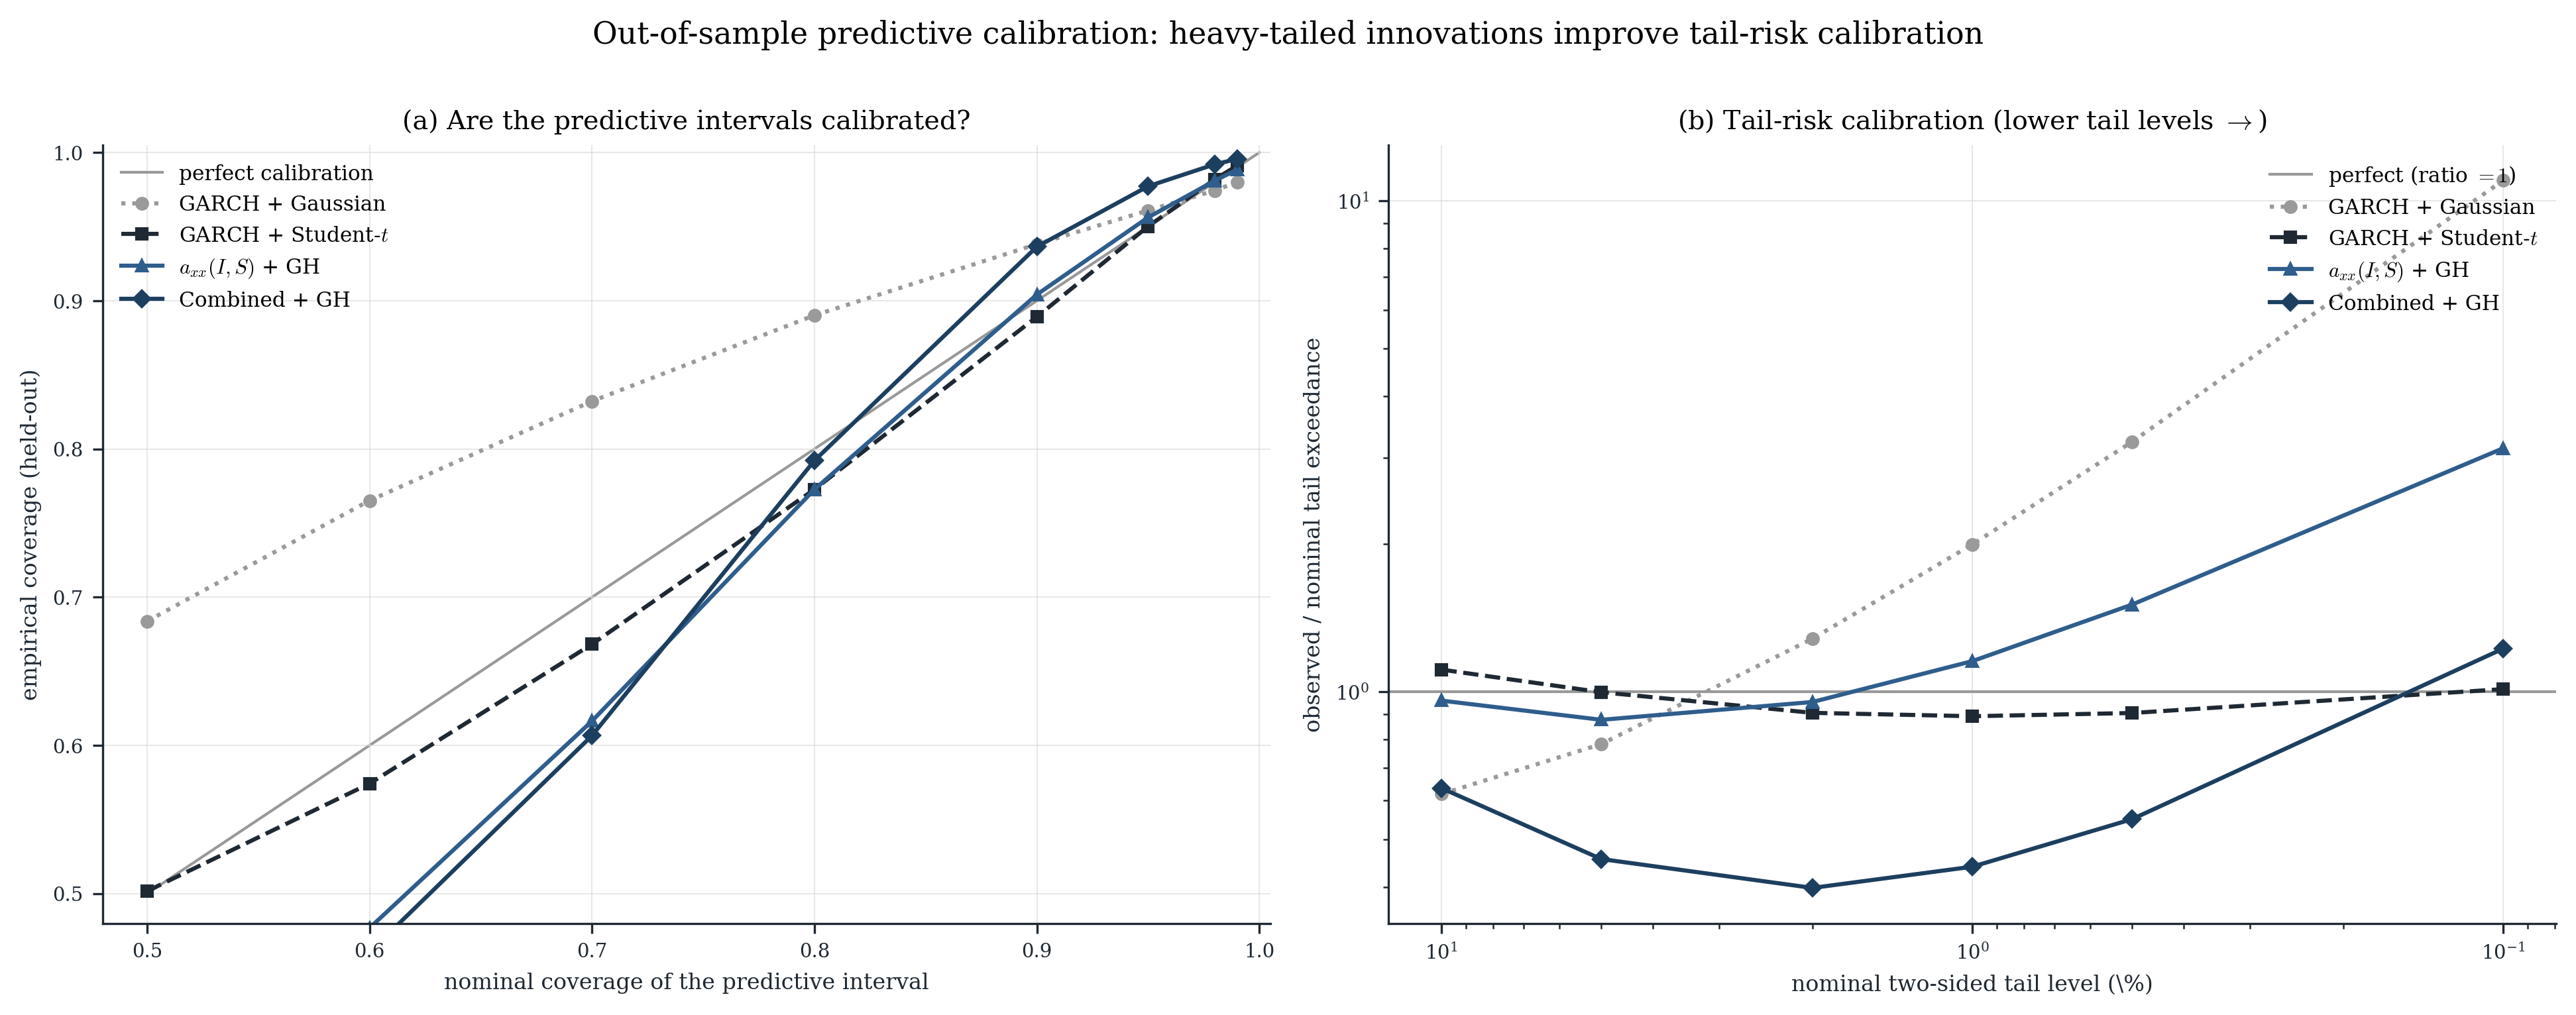
\includegraphics[width=\linewidth]{fig_garch_calibration.png}
\caption{Out-of-sample predictive calibration, pooled across all held-out moves and
instruments, for four models. Panel~(a): empirical against nominal coverage of the
central predictive interval; a perfectly calibrated model lies on the diagonal. A
Gaussian GARCH (grey, dotted) under-covers the tail; the Student-$t$ residual law and
the Generalized Hyperbolic models track the diagonal much more closely in the upper
tail. Panel~(b): the ratio of observed to nominal two-sided tail exceedance at levels
from $10\%$ down to $0.1\%$; a calibrated model lies on the line at one. The Gaussian
under-states the $0.1\%$ tail by a factor of about eleven; the book-state
$a_{xx}(I,S)$+GH model over-exceeds at the farthest tail (about three times nominal),
while Combined+GH is about $1.2$ times nominal at $0.1\%$. Supplements the VaR
backtest of Section~\ref{sub:var-backtest}.}
\label{fig:garchcal}
\end{figure}

\begin{figure}[!htbp]
\centering
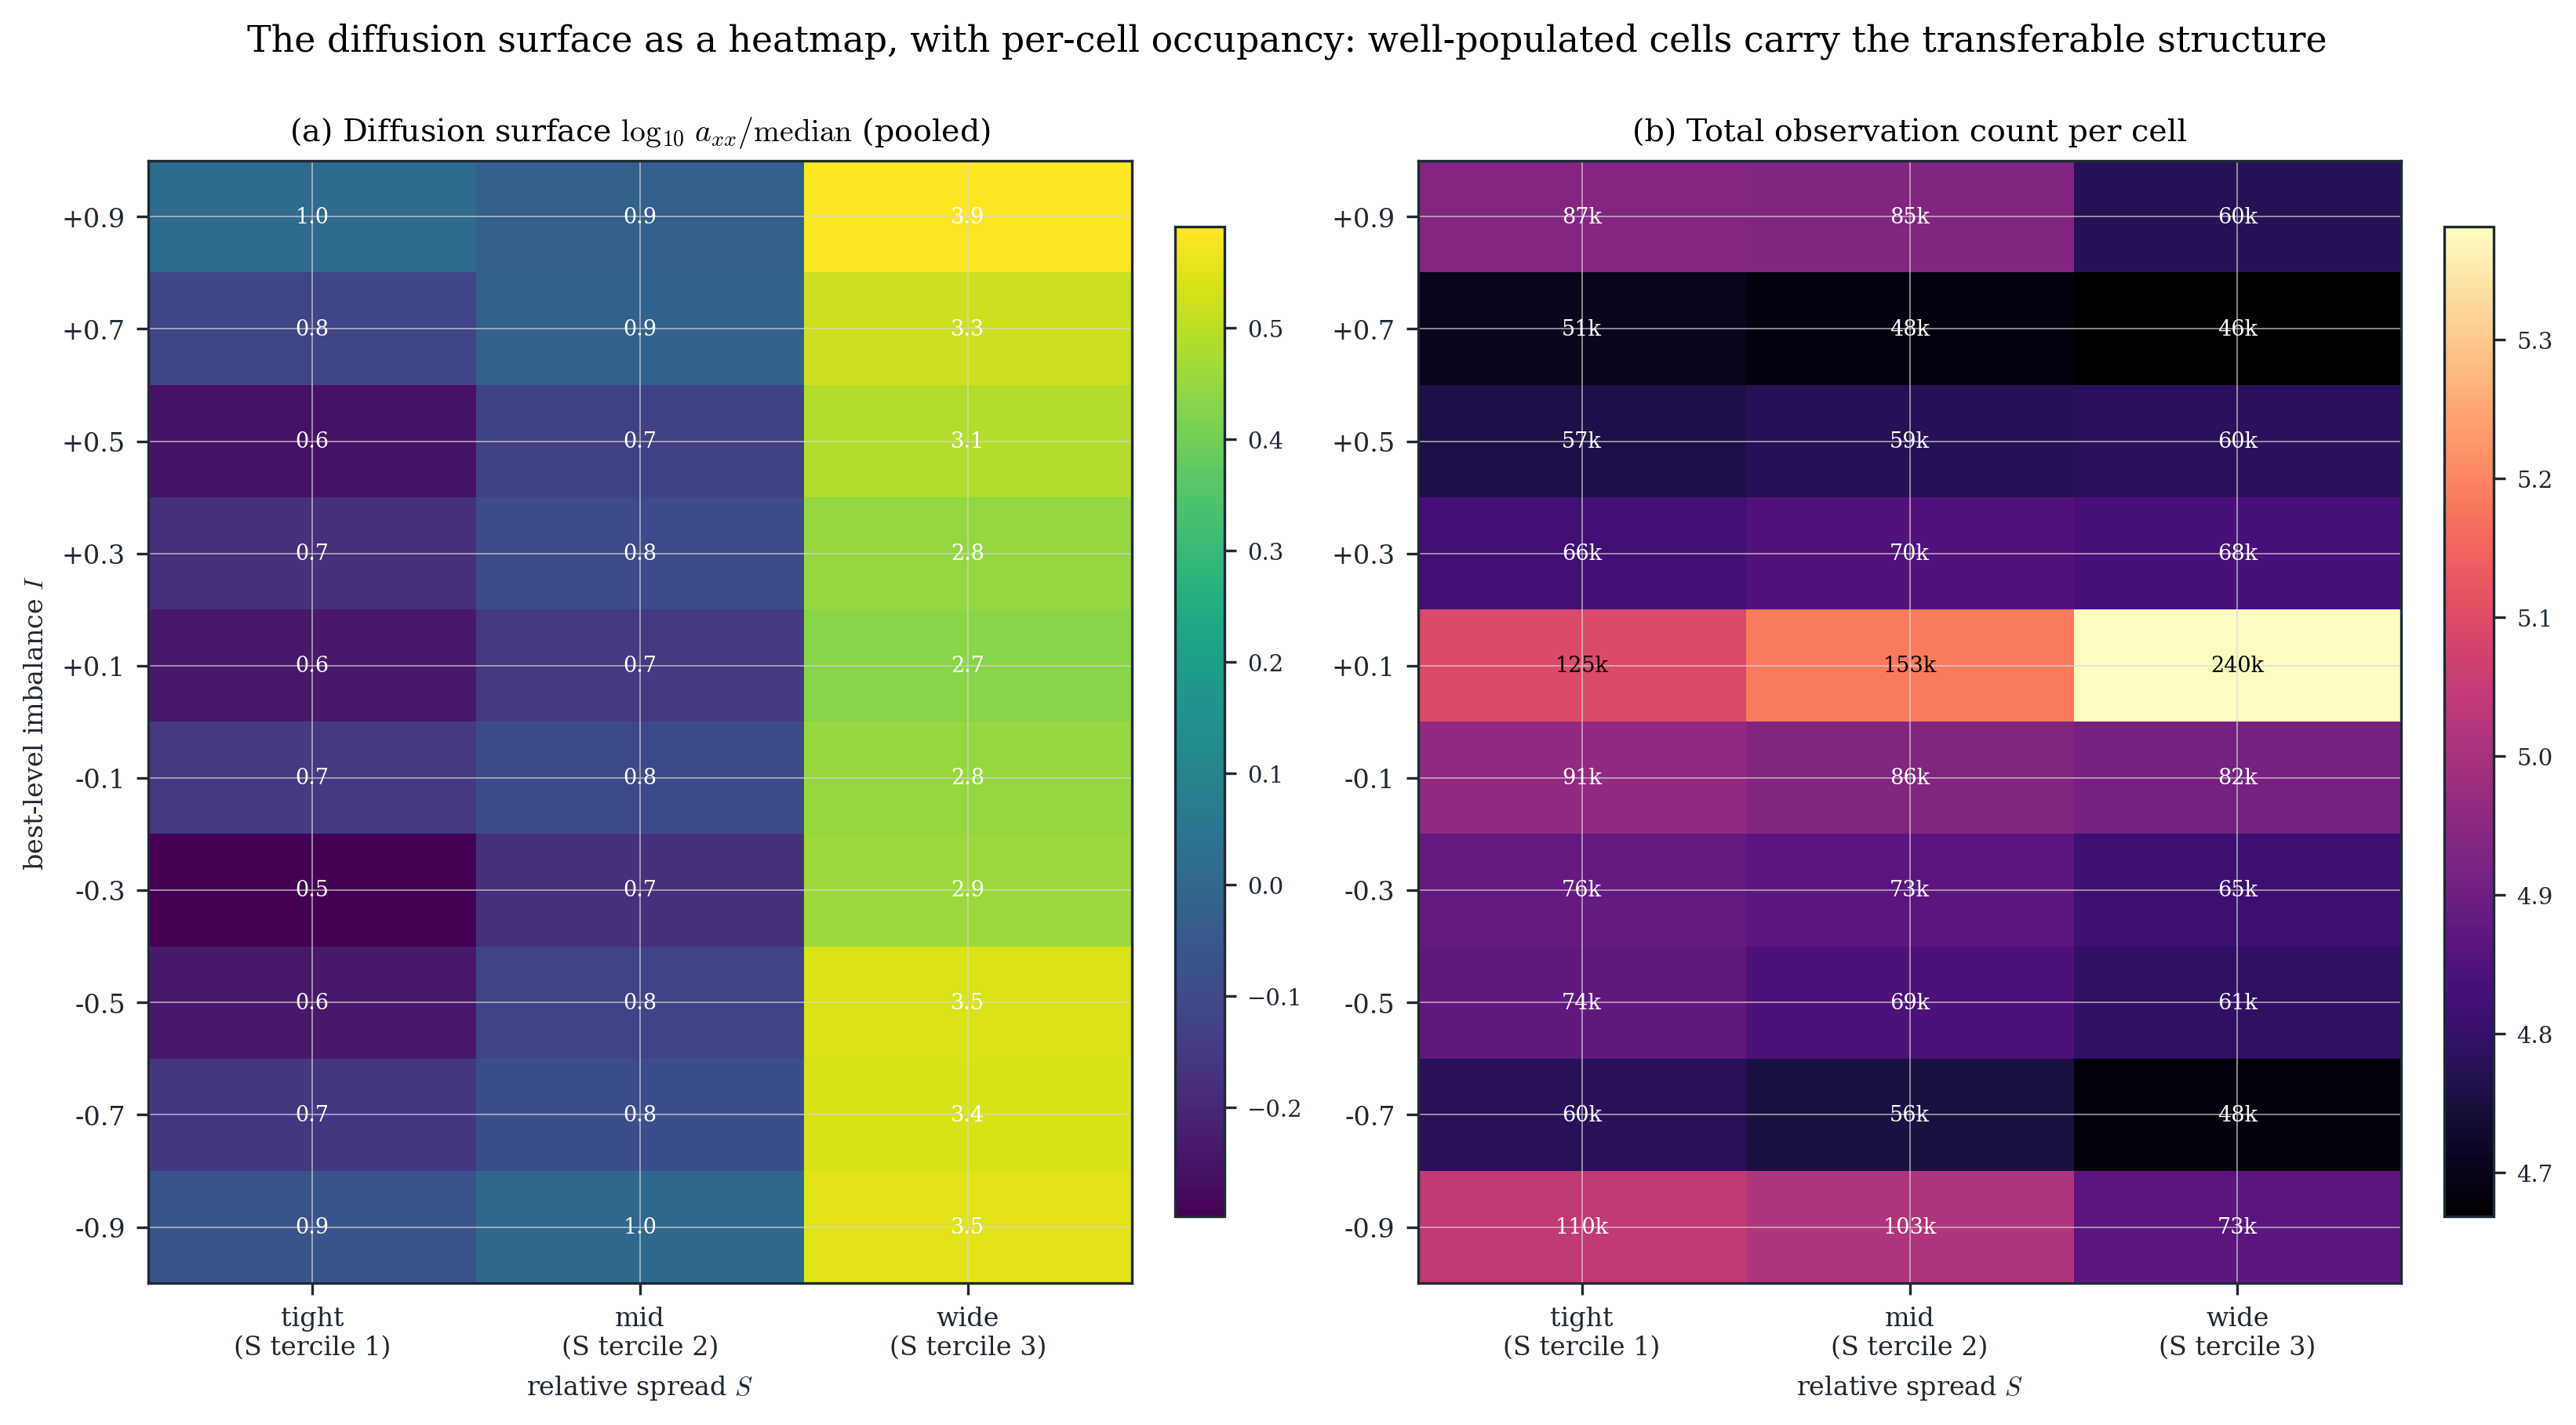
\includegraphics[width=0.9\linewidth]{fig_axx_heatmap_counts.png}
\caption{The microdiffusion surface with per-cell occupancy. Panel~(a): the pooled diffusion
surface $\log_{10}\axx$ (each instrument normalised to its own median, then pooled) over the
$10\times 3$ imbalance--spread grid, with each cell annotated by its value; the conditional
variance rises toward wide spreads and toward extreme imbalance of either sign. Panel~(b): the
total observation count per cell; the well-populated cells, the great majority, carry the
transferable structure, while the sparsest corners are those flagged in
Section~\ref{sec:robustness}. The heatmap makes the grid occupancy explicit, complementing the
smoothed three-dimensional rendering of Figure~\ref{fig:axx}.}
\label{fig:axxheatmap}
\end{figure}

\begin{figure}[!htbp]
\centering
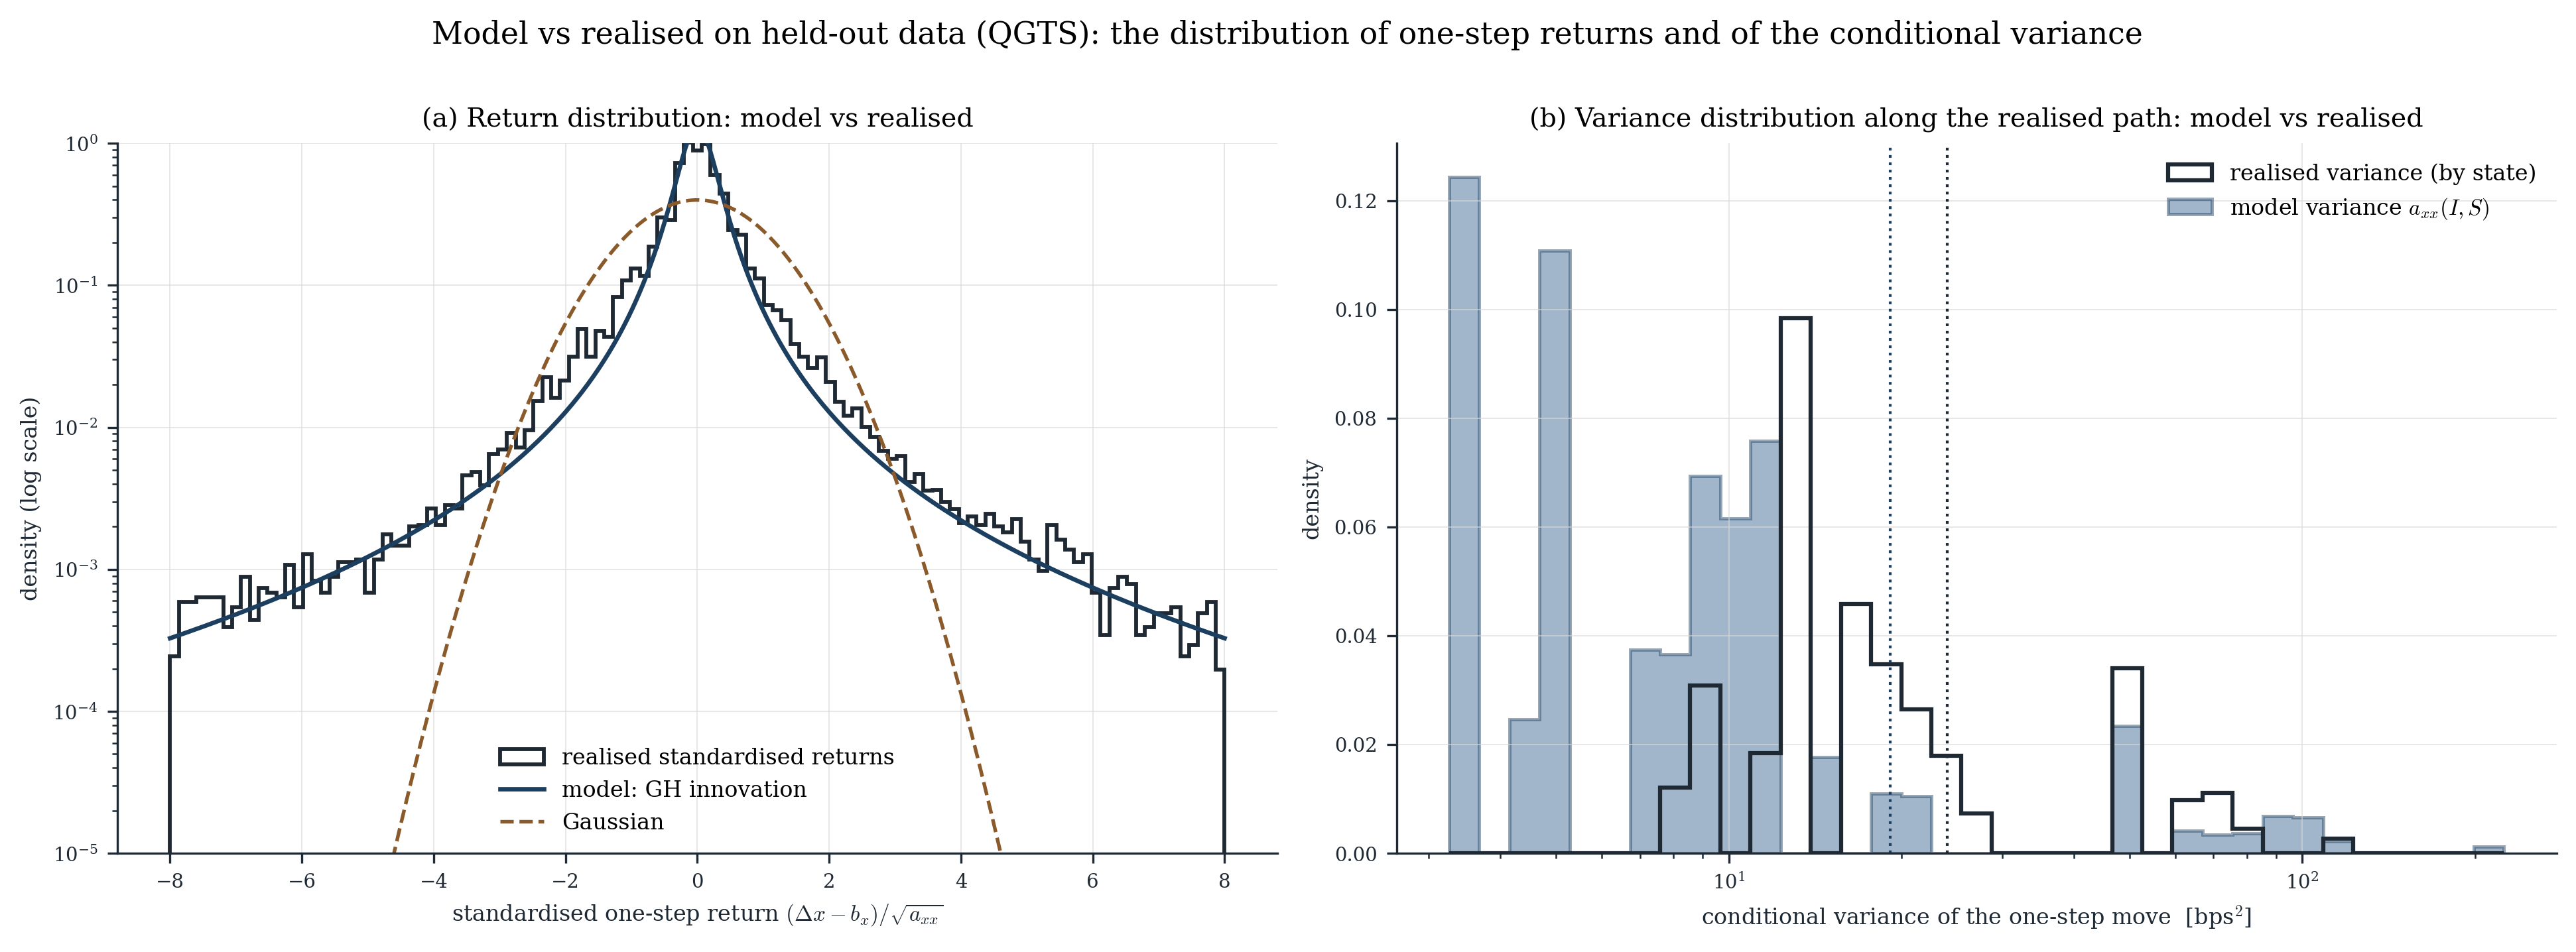
\includegraphics[width=\linewidth]{fig_model_vs_realized.png}
\caption{Model against realised data on one held-out instrument, distributionally.
Panel~(a): the density of standardised one-step returns $(\Delta x-b_x)/\sqrt{\axx}$
(histogram) against the fitted Generalized Hyperbolic innovation (solid) and a Gaussian
(dashed). The heavy-tailed law follows the empirical tail much more closely than the
Gaussian, although this single-instrument view is illustrative rather than inferential.
Panel~(b): the distribution of the conditional variance of the one-step move along the
realised state path, the model's $\axx(I,S)$ (filled) against the realised per-state
variance (outline), with medians marked. The model's variance distribution is close to
the realised one over the bulk, while the realised distribution is heavier in the far
right tail, consistent with volatility clustering that a static state surface does not
fully capture. The panels reproduce, for a single instrument, the pooled tail result of
Section~\ref{sub:res-gh} and the transfer result of Section~\ref{sub:res-axx}.}
\label{fig:modelreal}
\end{figure}

\begin{figure}[!htbp]
\centering
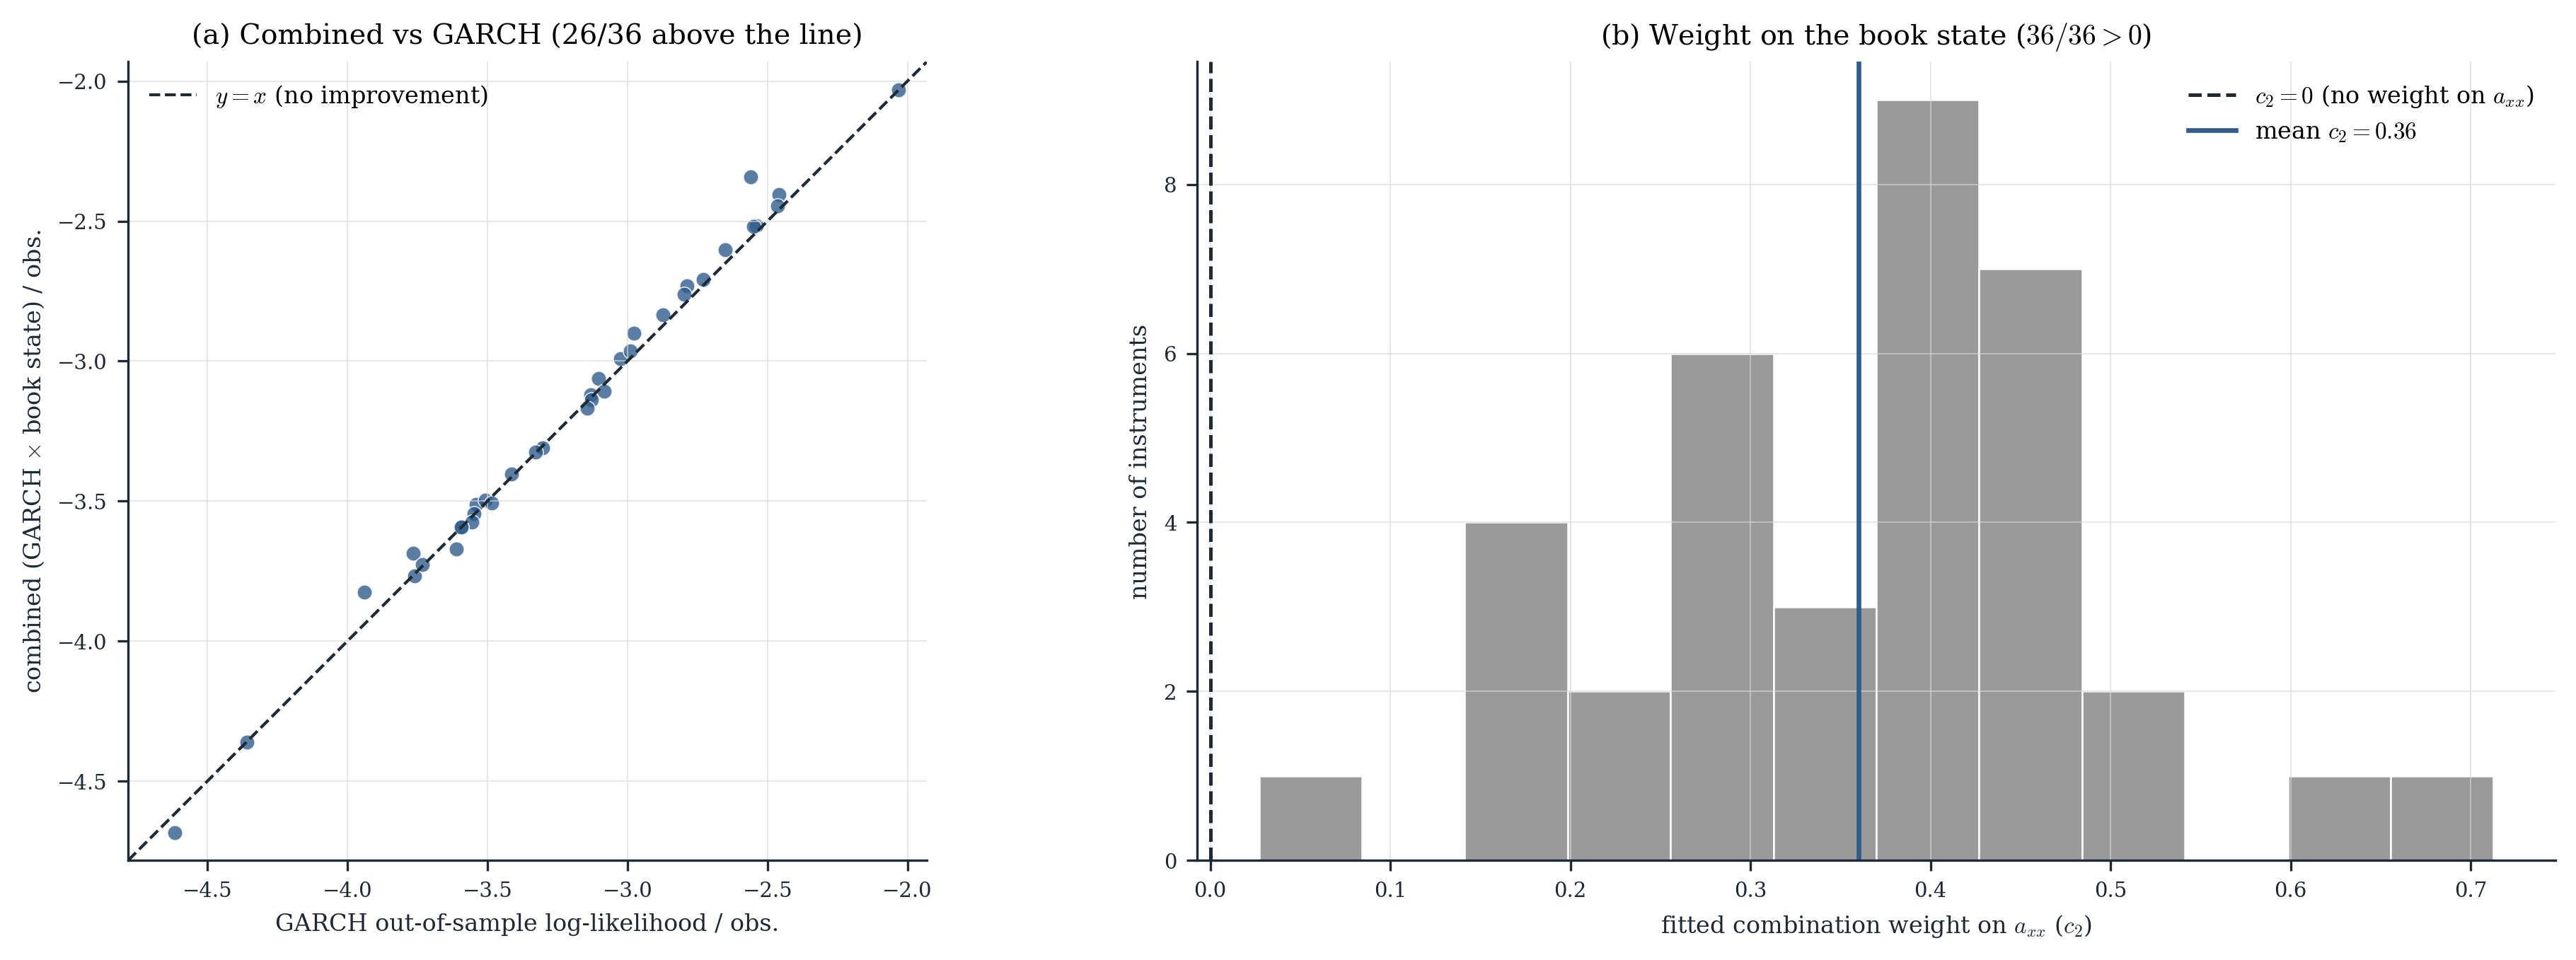
\includegraphics[width=\linewidth]{fig_garch_compare.png}
\caption{The book-state diffusion is complementary to, not a replacement for, GARCH.
Panel~(a): out-of-sample log-likelihood of the combined model against that of GARCH
alone, one point per instrument; points above the $45^\circ$ line are instruments for
which adding the book state improves on GARCH ($26$ of $36$). Panel~(b): the fitted
combination weight $c_2$ on $\axx(I,S)$, one per instrument; it is positive for every
instrument (mean $0.36$), even though the resulting forecast improvement is not positive
for every name, the optimiser consistently assigns weight to the book-state diffusion.}
\label{fig:garch}
\end{figure}

\begin{figure}[!htbp]
\centering
\includegraphics[width=\linewidth]{sde_tailknob_state.png}
\caption{The fitted tail thickness $\Var(G)$ by spread tercile (left) and by
imbalance bin (right). The tail thickness is nearly state-neutral, flat across
imbalance, with only a mild decline across the spread, in contrast to the scale
$\axx$, which varies across states by orders of magnitude.}
\label{fig:tailknob}
\end{figure}

\FloatBarrier
\section{Reproducibility}
\label{app:repro}

\subsection{Data provenance and cleaning}
\label{app:provenance}
The primary sample is reconstructed from the QSE MITCH message feed. The level-one book is
built from the exchange's authoritative best-bid/best-offer statistics messages, augmented
by the add/update/delete/execute order messages where they refine the touch; the
reconstruction reads the source feed read-only. We retain only well-formed level-one
records, positive, finite mid-price and positive best-level sizes, and discard
opening- and closing-auction states, halts, and crossed or empty books. The continuous
session is taken as $09{:}30$--$13{:}00$ local time, auctions and halts excluded. A
symbol-session enters the panel only if it carries at least $1{,}500$ cleaned events. The
estimation sample after cleaning is the $41$-instrument, $216$-session panel summarised in
Section~\ref{sub:venues}.

\subsection{Per-session update-count distribution}
\label{app:counts}
The $4.03$ million level-one updates are spread across $1{,}588$ instrument-sessions; the
median session carries $2{,}172$ updates, with a $10$th--$90$th percentile range of
$1{,}598$--$3{,}917$ and a maximum of $17{,}369$, and no retained session falls below one
hundred updates. The distribution is right-skewed, with a minority of liquid
instrument-sessions carrying a disproportionate share of the updates.

\subsection{Code and data availability}
\label{app:availability}
We will release the estimation and analysis code and the processed,
instrument-anonymised state--increment series on which every reported number is computed,
so that the tables and figures of Sections~\ref{sec:results} and the appendices can be
regenerated end to end. The raw exchange feed is subject to the venue's redistribution
terms and cannot be released directly; the cleaning and reconstruction pipeline that
produces the processed series from the feed is included with the code.

\end{document}
